\documentclass[twoside,9pt]{report}
\usepackage[a5paper]{geometry}
\usepackage{newpxmath}
%\usepackage{libertine} \usepackage[libertine]{newtxmath}
%\usepackage{kpfonts}
\usepackage{graphicx}
\usepackage{listings}
\usepackage[T1]{fontenc}
\usepackage{imakeidx}
\usepackage{marginnote}
\usepackage[table]{xcolor}
\lstset{
  showstringspaces=false,
  language=tcl,
  frame=lines,
  aboveskip=\bigskipamount,
  belowskip=\bigskipamount,
  numbers=left,
  numberstyle=\tiny,
  firstnumber=last,
  basicstyle=\small\ttfamily,
}
%\renewcommand{\thesection}{\arabic{section}}
\title{Into the Interpreter\\--with ConsTcl}
\author{Peter Lewerin}
\date{\today}
\makeatletter
\def\@makechapterhead#1{%
  \vspace*{50\p@}%
    {\parindent \z@ \raggedright \normalfont
      \ifnum \c@secnumdepth >\m@ne
        %\if@mainmatter
          %\huge\bfseries \@chapapp\space \thechapter
          \Huge\bfseries \thechapter.\space%
          %\par\nobreak
          %\vskip 20\p@
        %\fi
      \fi
      \interlinepenalty\@M
      \Huge \bfseries #1\par\nobreak
      \vskip 40\p@
   }}
\makeatother
\makeindex[intoc]
\counterwithout{footnote}{chapter}

\begin{document}
\pagestyle{headings}
\maketitle
\tableofcontents

\chapter{Introduction}
\label{introduction}
\section{To run the software}
\label{to-run-the-software}
\index{to run the software}


First things first. To run, source the file \textbf{constcl.tcl} (with
\textbf{schemebase.lsp} in the directory) in a Tcl console (I use
\textbf{tkcon}) and use the command \textbf{repl} for a primitive command
dialog. Source \textbf{all.tcl} to run the test suite (you need
\textbf{constcl.test} for that). The files can be found on GitHub/ConsTcl\footnote{See
\texttt{https://github.com/hoodiecrow/ConsTcl}}.

\section{Background}
\label{background}
\index{background}

It all started with Peter Norvig's Lisp emulator
Lispy\footnote{See \texttt{https://norvig.com/lispy.html}}. In January 2025 I
was inspired to port it to Tcl. The result was Thtcl\footnote{See
\texttt{https://github.com/hoodiecrow/thtcl}}. It had the same features and
limitations as Lispy, plus a couple that were due to shortcomings of Tcl, and I
came out of the experience feeling a bit dissatisfied. In the latter part of
January I embarked on a new project, ConsTcl, a true Lisp interpreter. In Tcl.

\subsection{About ConsTcl}
\label{about-constcl}

Compared to Lispy/Thtcl, ConsTcl has, (quote from Lispy), ``comments, quote and
quasiquote notation, \# literals, the derived expression types (such as cond,
derived from if, or let, derived from lambda), and dotted list notation.''
Again compared to Lispy/Thtcl, ConsTcl has the data types, quote, ``strings,
characters, booleans, ports, vectors.'' And pairs and procedures too. The
number of missing primitive procedures is in the tens, not the 100s. 

The completeness comes with a price: due to the sheer number of calls for each
action, ConsTcl is is fairly slow. On my cheap computer, the following code
(which calculates the factorial of 100) takes 0.03 seconds to run. That is ten
times slower than Lispy assuming that Norvig's computer is as slow as mine,
which is unlikely. So it's probably a factor of less than ten.

\begin{verbatim}
time {pe "(fact 100)"} 10
\end{verbatim}

ConsTcl is of course still limited. It doesn't come close to having call/cc or
tail recursion. It doesn't have exact/inexact numbers, or most of the numerical
tower. There is no memory management. Error reporting is spotty, and there is no
error recovery.

\subsection{About the book}
\label{about-the-book}


I like writing documentation, and occasionally I'm good at it. I like to
annotate the source code with bits of documentation, which I then extract and
put together using tools like \texttt{awk}. It looks like this:

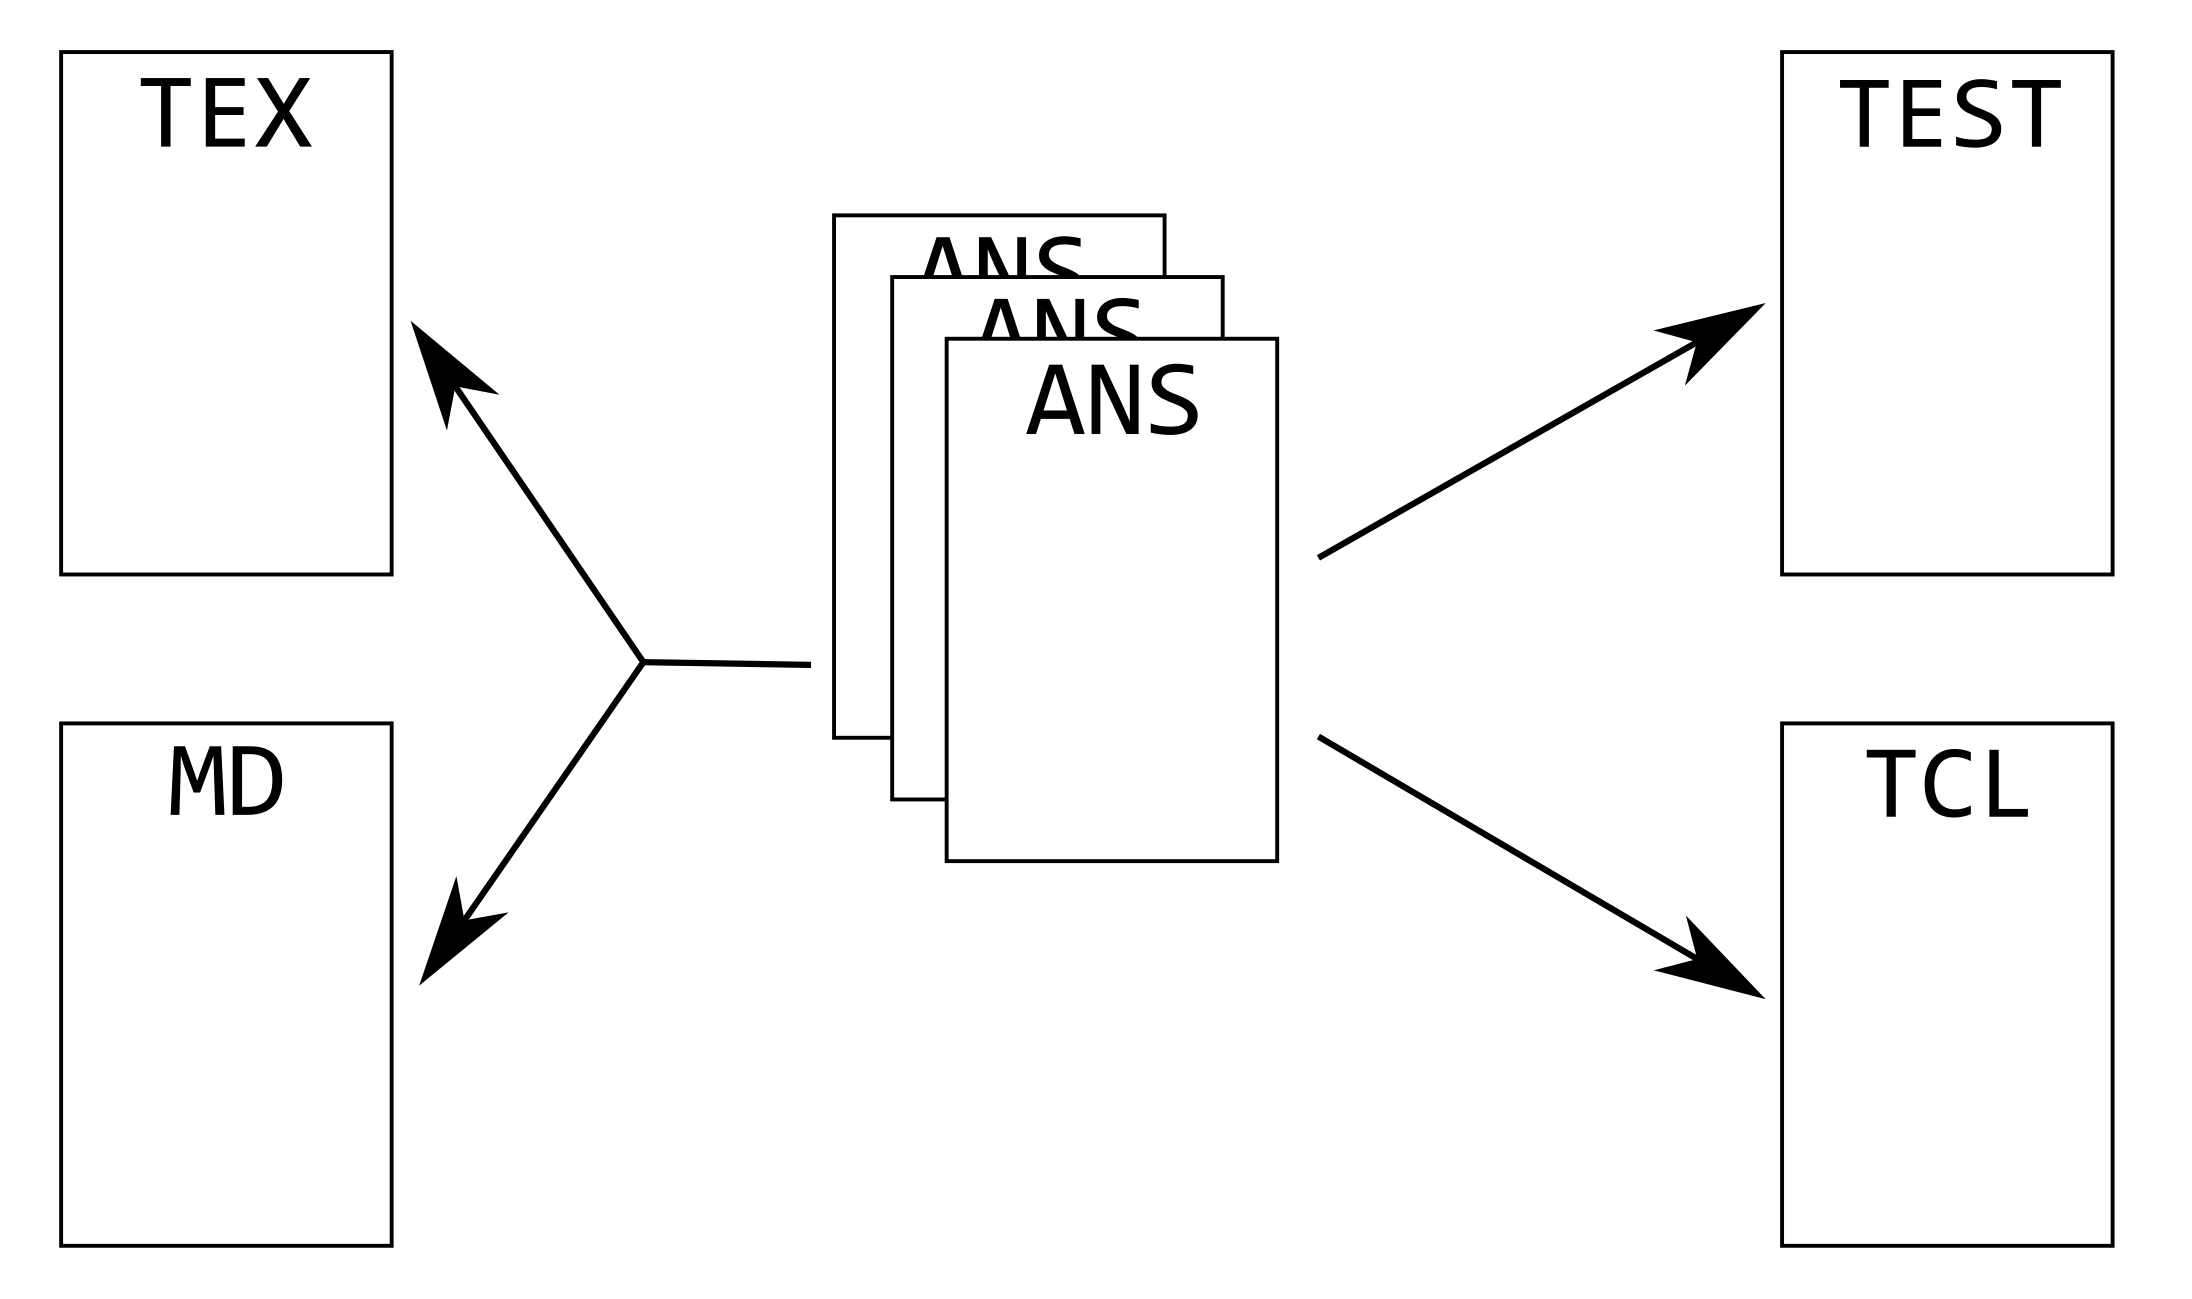
\includegraphics{images/document.png}

In the middle are a bunch of \texttt{.ans} files (ANnotated Source). These are
written with Vim. From the TT tags of those, I extract a \texttt{.test} file.
From the CB tags I extract \texttt{.tcl} source (or C source, as the case might
be). From all the tags except TT I extract formatted documentation in Markdown
and \LaTeX{} format. All these extractions are automated using \texttt{make}.
Figures are made with Inkscape.  I create a PDF document from the \LaTeX{}
source using TeXworks. On finishing up ConsTcl, it struck me that the
documentation for this piece of software was fit for a book.

\subsection{About the program listings}
\label{about-the-program-listings}

I have tried to write clear, readable code, but the page format forces me to
shorten lines. I have used two-space indents instead of four-space, a smaller
font, and broken off long lines with a \textbackslash\  at the end of the first
line (a so-called 'tucked-in tail'). Neither of these measures improve
readability, but the alternative is overwriting the margins. Not all broken
lines have the \textbackslash: some are broken inside a
\texttt{\{}\ldots\texttt{\}} block, and some right after a \texttt{^^5b}.

\subsection{About me}
\label{about-me}

I'm a 60 year old former system manager who has been active in programming
since 1979. Currently, since around 25 years, my language of choice is the
rather marginal Tcl (it's not even in the 100 most used languages). Tcl suits
me, and there are things that one can do in Tcl that one can't easily do in
other languages. Lisp is a runner-up in my affections, a language that
fascinates me but doesn't fit my brain very well (though I have written one
large piece of software in AutoLisp, a CAD subsystem for designing drilling
boxes).

In addition to my terms as programmer and system manager, I have worked as a
teacher (teaching C/C++ in upper secondary school) and for a short while I
produced textbooks for the department for information technology at
the University of Skövde. I've also been active writing answers at
question-and-answer sites on the web, mainly Stack Overflow.

\subsection{About time}
\label{about-time}

I'd like to thank

\begin{itemize}
\item my children and their lifemates for being awesome.

\item my ex-wife for supporting the printing of the book financially, and, well, for being awesome too.

\item all the wonderful people in my life for being there.
\end{itemize}

And now let's journey into the Interpreter.
\chapter{Initial declarations}
\label{initial-declarations}


First, I need to create the namespace that will be used for most identifiers:

\begin{lstlisting}
namespace eval ::constcl {}
\end{lstlisting}
\section{Utility commands}
\label{utility-commands}
\index{utility commands}


Next, some procedures that make my life as developer somewhat easier.



\textbf{reg} procedure


\texttt{reg} registers selected built-in procedures in the definitions register\index{definitions register}. That way I don't need to manually keep track of and list procedures. The definitions register's contents will eventually get dumped into the standard library (see page \pageref{environment-startup}).


You can call \texttt{reg} with two values: \emph{key} and \emph{val}. \emph{Key} is the string that will eventually become the lookup symbol in the standard library, and \emph{val} is the name of the Tcl command that will carry out the procedure. If you don't give a value for \emph{val}, \texttt{reg} creates a value by prepending the \texttt{::constcl::} namespace to the \emph{key} value, which is sufficient 99\% of the time.

\noindent\begin{tabular}{ |p{1.5cm} p{8cm}| }
\hline
\rowcolor[HTML]{CCCCCC} \multicolumn{2}{|l|}{\bf reg (internal)} \\
key & a Tcl string \\
?val? & a Tcl string \\
\textit{Returns:} & nothing \\
\hline
\end{tabular}
\index{reg}
\begin{lstlisting}
proc ::reg {key args} {
  if {[llength $args]} {
    lassign $args val
  } else {
    set val ::constcl::$key
  }
  dict set ::constcl::defreg $key $val
  return
}
\end{lstlisting}
\subsubsection{Procedures, functions, and commands: an aside}
\label{procedures,-functions,-and-commands:-an-aside}


I use all of these terms for the subroutines in ConsTcl. I try to stick to procedure, because that's the standard term in R5RS\footnote{Revised5 Report on the Algorithmic Language Scheme, Scheme's standardization document}. Still, they usually pass useful values back to the caller, so technically they're functions. Lastly, I'm programming in Tcl here, and the usual term for these things is `commands' in Tcl.


And the `internal/public' distinction is probably a misnomer (an aside within an aside, here). What it means is that `public' procedures can be called from Lisp code being interpreted, and the others cannot. They are for use in the infrastructure around the interpreter, including in implementing the `public' procedures. Another way to put it is that procedures registered by \texttt{reg} are `public' and those who aren't are `internal'.



\textbf{regmacro} procedure


ConsTcl has macros\index{macro}, i.e. succinct syntactic forms that are rewritten to concrete--but more verbose--forms. The evaluator passes macro forms to a command for expansion before they are fully processed. \texttt{regmacro} registers macro names in the macro list, so the evaluator knows what to expand.

\noindent\begin{tabular}{ |p{1.5cm} p{8cm}| }
\hline
\rowcolor[HTML]{CCCCCC} \multicolumn{2}{|l|}{\bf regmacro (internal)} \\
name & a Tcl string \\
\textit{Returns:} & nothing \\
\hline
\end{tabular}
\index{regmacro}
\begin{lstlisting}
proc ::regmacro {name} {
  lappend ::constcl::macrolist $name
  return
}
\end{lstlisting}


\textbf{pn} procedure


\texttt{pn} stands for 'procedure name'. When called, tells the caller the name of its command. I use it for error messages so the error message can automagically tell the user which command failed.

\index{pn}
\noindent\begin{tabular}{ |p{1.5cm} p{8cm}| }
\hline
\rowcolor[HTML]{CCCCCC} \multicolumn{2}{|l|}{\bf pn (internal)} \\
\textit{Returns:} & a Tcl string \\
\hline
\end{tabular}
\begin{lstlisting}
proc ::pn {} {
  lindex [split [lindex [info level -1] 0] :] end
}
\end{lstlisting}


\textbf{typeof?} procedure


\texttt{typeof?} looks at a value's type and reports if it is the same as the given type. To be certain, it looks at the value in two ways: once assuming that the value is a ConsTcl object, and once assuming that the value is an interpreter\footnote{the Tcl interpreter, not ConsTcl} alias for a ConsTcl object. If one of those affirms the type, the procedure returns \texttt{\#t}.


By Scheme convention, predicates\footnote{See \texttt{https://en.wikipedia.org/wiki/Boolean-valued\_function}}\index{predicate} (procedures that return either \texttt{\#t} or \texttt{\#f}) have '?' at the end of their name. Some care is necessary when calling Scheme predicates from Tcl code (the Tcl \texttt{if} command expects 1 or 0 as truth values). Example:


\texttt{if \{[typeof? \$v Dot]\} \ldots }


will not do, but


\texttt{if \{[typeof? \$v Dot] ne "\#f"\} \ldots }


works.

\noindent\begin{tabular}{ |p{1.5cm} p{8cm}| }
\hline
\rowcolor[HTML]{CCCCCC} \multicolumn{2}{|l|}{\bf typeof? (internal)} \\
val & a Lisp value \\
type & a Tcl string \\
\textit{Returns:} & a boolean \\
\hline
\end{tabular}
\index{typeof?}
\begin{lstlisting}
proc ::constcl::typeof? {val type} {
  if {[info object isa typeof $val $type]} {
    return #t
  } elseif {[info object isa typeof \
      [interp alias {} $val] $type]} {
    return #t
  } else {
    return #f
  }
}
\end{lstlisting}


\textbf{in-range} procedure


This one is a little bit of both, a utility function that is also among the builtins in the library. It started out as a one-liner by Donal K. Fellows\index{Fellows, Donal}, but has grown a bit since then to suit my needs.


The plan is to arrange a sequence of numbers, given one, two or three ConsTcl Number objects. If one is passed to the procedure, it is used as the end of the sequence: the sequence will end just before it. If two numbers are passed, the first one becomes the start of the sequence: the first number in it. The second number will become the end of the sequence. If three numbers are passed, they become start, end, and step, i.e. how much is added to the current number to find next number in the sequence.

\noindent\begin{tabular}{ |p{1.5cm} p{8cm}| }
\hline
\rowcolor[HTML]{CCCCCC} \multicolumn{2}{|l|}{\bf in-range (public)} \\
x & a number \\
?e? & a number \\
?t? & a number \\
\textit{Returns:} & a Lisp list of numbers \\
\hline
\end{tabular}
\index{in-range}
\begin{lstlisting}
reg in-range
 
proc ::constcl::in-range {x args} {
  set start 0
  set step 1
  switch [llength $args] {
    0 {
      set e $x
      set end [$e numval]
    }
    1 {
      set s $x
      lassign $args e
      set start [$s numval]
      set end [$e numval]
    }
    2 {
      set s $x
      lassign $args e t
      set start [$s numval]
      set end [$e numval]
      set step [$t numval]
    }
  }
  set res $start
  while {$step > 0 && $end > [incr start $step] ||
      $step < 0 && $end < [incr start $step]} {
    lappend res $start
  }
  return [list {*}[lmap r $res {MkNumber $r}]]
}
\end{lstlisting}
\section{Testing commands}
\label{testing-commands}
\index{testing commands}


\textbf{pew} procedure


\texttt{pew} was originally named \texttt{pep} after the sequence parse-eval-print. Now it's named for parse-eval-write. It reads and evals an expression, and writes the result. It's the most common command in the test cases, since it allows me to write code directly in Scheme, get it evaled and get to see proper Lisp output from it.

\noindent\begin{tabular}{ |p{1.5cm} p{8cm}| }
\hline
\rowcolor[HTML]{CCCCCC} \multicolumn{2}{|l|}{\bf pew (internal)} \\
str & a Tcl string, Lisp string, or an input buffer \\
\textit{Returns:} & nothing \\
\hline
\end{tabular}
\index{pew}
\begin{lstlisting}
proc ::pew {str} {
  ::constcl::write [
    ::constcl::eval [
      ::constcl::parse $str]]
}
\end{lstlisting}


\textbf{pw} procedure


\texttt{pw} is a similar command, except it doesn't eval the expression. It just writes what is parsed. It is useful for tests when the evaluator can't (yet) evaluate the form, but I can still check if it gets read and written correctly.

\index{pw}
\noindent\begin{tabular}{ |p{1.5cm} p{8cm}| }
\hline
\rowcolor[HTML]{CCCCCC} \multicolumn{2}{|l|}{\bf pw (internal)} \\
str & a Tcl string, Lisp string, or an input buffer \\
\textit{Returns:} & nothing \\
\hline
\end{tabular}
\begin{lstlisting}
proc ::pw {str} {
  ::constcl::write [
    ::constcl::parse $str]
}
\end{lstlisting}


\textbf{rw} procedure


\texttt{rw} is the reading variant of \texttt{pw}, that is it takes in its input via a port instead of an input buffer. The distinction mattered more when the input library was being written. The procedure just writes what is read.

\noindent\begin{tabular}{ |p{1.5cm} p{8cm}| }
\hline
\rowcolor[HTML]{CCCCCC} \multicolumn{2}{|l|}{\bf rw (internal)} \\
?port? & an input port \\
\textit{Returns:} & nothing \\
\hline
\end{tabular}
\index{rw}
\begin{lstlisting}
proc ::rw {args} {
  ::constcl::write [
    ::constcl::read {*}$args]
}
\end{lstlisting}


\textbf{pe} procedure


\texttt{pe} is also similar, but it doesn't write the expression. It just evaluates what is read. That way I get a value object which I can pass to another command, or pick apart in different ways.

\noindent\begin{tabular}{ |p{1.5cm} p{8cm}| }
\hline
\rowcolor[HTML]{CCCCCC} \multicolumn{2}{|l|}{\bf pe (internal)} \\
str & a Tcl string, Lisp string, or an input buffer \\
\textit{Returns:} & a Lisp value \\
\hline
\end{tabular}
\index{pe}
\begin{lstlisting}
proc ::pe {str} {
  ::constcl::eval [
    ::constcl::parse $str]
}
\end{lstlisting}


\textbf{re} procedure


\texttt{re} is like \texttt{pe}, but it reads from a port instead of an input buffer. It evaluates what is read.

\noindent\begin{tabular}{ |p{1.5cm} p{8cm}| }
\hline
\rowcolor[HTML]{CCCCCC} \multicolumn{2}{|l|}{\bf re (internal)} \\
?port? &  \\
val &  \\
\hline
\end{tabular}
\index{re}
\begin{lstlisting}
proc ::re {args} {
  ::constcl::eval [
    ::constcl::read {*}$args]
}
\end{lstlisting}


\textbf{p} procedure


\texttt{p} only parses the input, returning an expression object.

\noindent\begin{tabular}{ |p{1.5cm} p{8cm}| }
\hline
\rowcolor[HTML]{CCCCCC} \multicolumn{2}{|l|}{\bf p (internal)} \\
str & a Tcl string, Lisp string, or an input buffer \\
\textit{Returns:} & an expression \\
\hline
\end{tabular}
\index{p}
\begin{lstlisting}
proc ::p {str} {
  ::constcl::parse $str
}
\end{lstlisting}


\textbf{e} procedure


\texttt{e} is another single-action procedure, evaluating an expression and returning a value.

\index{e}
\noindent\begin{tabular}{ |p{1.5cm} p{8cm}| }
\hline
\rowcolor[HTML]{CCCCCC} \multicolumn{2}{|l|}{\bf e (internal)} \\
expr & an expression \\
\textit{Returns:} & a Lisp value \\
\hline
\end{tabular}
\begin{lstlisting}
proc ::e {expr} {
  ::constcl::eval $expr
}
\end{lstlisting}


\textbf{w} procedure


\texttt{w} is the third single-action procedure, printing a value and that's all.

\noindent\begin{tabular}{ |p{1.5cm} p{8cm}| }
\hline
\rowcolor[HTML]{CCCCCC} \multicolumn{2}{|l|}{\bf w (internal)} \\
val & a Lisp value \\
\textit{Returns:} & nothing \\
\hline
\end{tabular}
\index{w}
\begin{lstlisting}
proc ::w {val} {
  ::constcl::write $val
}
\end{lstlisting}


\textbf{r} procedure


\texttt{r} is an extra single-action procedure, reading from default input or from a port and returning an expression object.

\noindent\begin{tabular}{ |p{1.5cm} p{8cm}| }
\hline
\rowcolor[HTML]{CCCCCC} \multicolumn{2}{|l|}{\bf r (internal)} \\
?port? & an input port \\
\textit{Returns:} & an expression \\
\hline
\end{tabular}
\index{r}
\begin{lstlisting}
proc ::r {args} {
  ::constcl::read {*}$args
}
\end{lstlisting}


\textbf{prw} procedure


\texttt{prw} reads an expression, resolves defines, and writes the result. It was handy during the time I was porting the 'resolve local defines' section.

\noindent\begin{tabular}{ |p{1.5cm} p{8cm}| }
\hline
\rowcolor[HTML]{CCCCCC} \multicolumn{2}{|l|}{\bf prw (internal)} \\
str & a Tcl string, Lisp string, or an input buffer \\
\textit{Returns:} & nothing \\
\hline
\end{tabular}
\index{prw}
\begin{lstlisting}
proc ::prw {str} {
  set expr [::constcl::parse $str]
  set expr [::constcl::resolve-local-defines \
    [::constcl::cdr $expr]]
  ::constcl::write $expr
}
\end{lstlisting}


\textbf{pxw} procedure


\texttt{pxw} attempts to macro-expand whatever it reads, and writes the result. I know that 'expand' doesn't start with an 'x'. Again, this command's heyday was when I was developing the macro facility.

\noindent\begin{tabular}{ |p{1.5cm} p{8cm}| }
\hline
\rowcolor[HTML]{CCCCCC} \multicolumn{2}{|l|}{\bf pxw (internal)} \\
str & a Tcl string, Lisp string, or an input buffer \\
\textit{Returns:} & nothing \\
\hline
\end{tabular}
\index{pxw}
\begin{lstlisting}
proc ::pxw {str} {
  set expr [::constcl::parse $str]
  set expr [::constcl::expand-macro $expr \
    ::constcl::global_env]
  ::constcl::write $expr
}
\end{lstlisting}
\section{The NIL class}
\label{the-nil-class}
\index{the nil class}


The \texttt{NIL} class has one object: the empty list called \texttt{\#NIL}. It is also base class for many other type classes.

\index{NIL}
\begin{lstlisting}
catch { ::constcl::NIL destroy }
 
oo::singleton create ::constcl::NIL {
  method boolval {} {
    return #t
  }
  method car {} {
    ::error "PAIR expected"
  }
  method cdr {} {
    ::error "PAIR expected"
  }
  method set-car! {v} {
    ::error "PAIR expected"
  }
  method set-cdr! {v} {
    ::error "PAIR expected"
  }
  method numval {} {
    ::error "NUMBER expected"
  }
  method write {handle} {
    puts -nonewline $handle "()"
  }
  method display {handle} {
    my write $handle
  }
  method show {} {
    format "()"
  }
}
\end{lstlisting}


\textbf{null?} procedure


The \texttt{null?} standard predicate recognizes the empty list.

\noindent\begin{tabular}{ |p{1.5cm} p{8cm}| }
\hline
\rowcolor[HTML]{CCCCCC} \multicolumn{2}{|l|}{\bf null? (public)} \\
val & a Lisp value \\
\textit{Returns:} & a boolean \\
\hline
\end{tabular}
\index{null?}
\begin{lstlisting}
reg null?
 
proc ::constcl::null? {val} {
  if {$val eq "#NIL"} {
    return #t
  } else {
    return #f
  }
}
\end{lstlisting}
\section{The classes Dot, Unspecified, Undefined, and EndOfFile}
\label{the-classes-dot,-unspecified,-undefined,-and-endoffile}
\index{the classes dot, unspecified, undefined, and endoffile}


\textbf{Dot} class


The \texttt{Dot} class is a helper class for the parser.

\index{Dot}
\begin{lstlisting}
catch { ::constcl::Dot destroy }
 
oo::class create ::constcl::Dot {
  method mkconstant {} {}
  method write {handle} {
    puts -nonewline $handle "."
  }
  method display {handle} {
    my write $handle
  }
}
\end{lstlisting}


\textbf{dot?} procedure


\texttt{dot?} is a type predicate that checks for membership in the type \texttt{Dot}.

\noindent\begin{tabular}{ |p{1.5cm} p{8cm}| }
\hline
\rowcolor[HTML]{CCCCCC} \multicolumn{2}{|l|}{\bf dot? (internal)} \\
val & a Lisp value \\
\textit{Returns:} & a boolean \\
\hline
\end{tabular}
\index{dot?}
\begin{lstlisting}
proc ::constcl::dot? {val} {
  typeof? $val "Dot"
}
\end{lstlisting}


\textbf{Unspecified} class


The \texttt{Unspecified} class is for unspecified things. It was created to facilitate porting of code from `Scheme 9 from Empty Space'\index{S9fES}.

\index{Unspecified}
\begin{lstlisting}
catch { ::constcl::Unspecified destroy }
 
oo::class create ::constcl::Unspecified {
  method mkconstant {} {}
  method write {handle} {
    puts -nonewline $handle "#<unspecified>"
  }
  method display {handle} {
    my write $handle
  }
}
\end{lstlisting}


\textbf{Undefined} class


The \texttt{Undefined} class is for undefined things. Also a S9fES support class.

\index{Undefined}
\begin{lstlisting}
catch { ::constcl::Undefined destroy }
 
oo::class create ::constcl::Undefined {
  method mkconstant {} {}
  method write {handle} {
    puts -nonewline $handle "#<undefined>"
  }
  method display {handle} {
    my write $handle
  }
}
\end{lstlisting}


\textbf{EndOfFile} class


The \texttt{EndOfFile} class is for end-of-file\index{end of file} conditions.

\index{EndOfFile}
\begin{lstlisting}
catch { ::constcl::EndOfFile destroy }
 
oo::class create ::constcl::EndOfFile {
  method mkconstant {} {}
  method write {handle} {
    puts -nonewline $handle "#<end-of-file>"
  }
  method display {handle} {
    my write $handle
  }
}
\end{lstlisting}
\index{eof?}
\begin{lstlisting}
proc eof? {val} {
  if {$val eq "#EOF"} {
    return #t
  } else {
    return #f
  }
}
\end{lstlisting}
\section{The error and check procedures}
\label{the-error-and-check-procedures}
\index{the error and check procedures}


\textbf{error} procedure


\texttt{error} is used to signal an error, with \emph{msg} being a message string and the optional arguments being values to show after the message.

\noindent\begin{tabular}{ |p{1.5cm} p{8cm}| }
\hline
\rowcolor[HTML]{CCCCCC} \multicolumn{2}{|l|}{\bf error (public)} \\
msg & a message string \\
?exprs? & some expressions \\
\textit{Returns:} & -don't care- \\
\hline
\end{tabular}
\index{error}
\begin{lstlisting}
reg error
 
proc ::constcl::error {msg args} {
  if {[llength $args]} {
    lappend msg "("
    set times 0
    foreach arg $args {
      if {$times} {
        ::append msg " "
      }
      ::append msg [$arg show]
      incr times
    }
    lappend msg ")"
  }
  ::error $msg
}
\end{lstlisting}


\textbf{check} procedure


\texttt{check} does a check (typically a type check) on something and throws an error if it fails.

\index{check}
\begin{lstlisting}
proc ::constcl::check {cond msg} {
  if {[uplevel $cond] eq "#f"} {
    ::error [
      uplevel [
        ::list subst [
          ::string trim $msg]]]
  }
}
\end{lstlisting}
\section{The atom? predicate}
\label{the-atom?-predicate}
\index{the atom? predicate}


\textbf{atom?} procedure


There are two kinds of data in Lisp: lists\index{list} and atoms\index{atom}. Lists are collections of lists and atoms. Atoms are instances of types such as booleans, characters, numbers, ports, strings, symbols, and vectors. \texttt{Atom?} recognizes an atom by checking for membership in any one of the atomic types.

\noindent\begin{tabular}{ |p{1.5cm} p{8cm}| }
\hline
\rowcolor[HTML]{CCCCCC} \multicolumn{2}{|l|}{\bf atom? (public)} \\
val & a Lisp value \\
\textit{Returns:} & a boolean \\
\hline
\end{tabular}
\index{atom?}
\begin{lstlisting}
reg atom? ::constcl::atom?
 
proc ::constcl::atom? {val} {
  foreach type {symbol number string
      char boolean vector port eof} {
    if {[$type? $val] eq "#t"} {
      return #t
    }
  }
  return #f
}
\end{lstlisting}
\chapter{Input}
\label{input}


The first thing an interpreter must be able to do is to take in the user's code and data input\index{input}, whether from the keyboard or from a source file. \texttt{read} represents the interpreter's main input facility. The \texttt{read-} procedures read from standard input, or--if a port is provided--from the port's channel.

\section{Parsing}
\label{parsing}
\index{parsing}
\subsection{The parsing process}
\label{the-parsing-process}
\index{the parsing process}


Parsing\footnote{See \texttt{https://en.wikipedia.org/wiki/Parsing}}\index{parsing}, or syntactic analysis, is analyzing a sequence of letters, digits, and other characters, conforming to the rules of \emph{external representation}\index{external representation}. The result of parsing is an \emph{expression}\index{expression} in internal form.


The parsing process translates an expression from external representation to internal representation. The external representation is a 'recipe' for an expression that expresses it in a unique way.


For example, the external representation for a vector is a sharp sign (\texttt{\#}), a left parenthesis (\texttt{(}), the external representation for some values, and a right parenthesis (\texttt{)}). When the reader or parser is working through input, a \texttt{\#(} symbol signals that a vector structure is being read. A number of subexpressions for the elements of the vector follow, and then a closing parenthesis \texttt{)} signals that the vector is done. The elements are saved in vector memory and the vector gets the address to the first element and the number of elements.

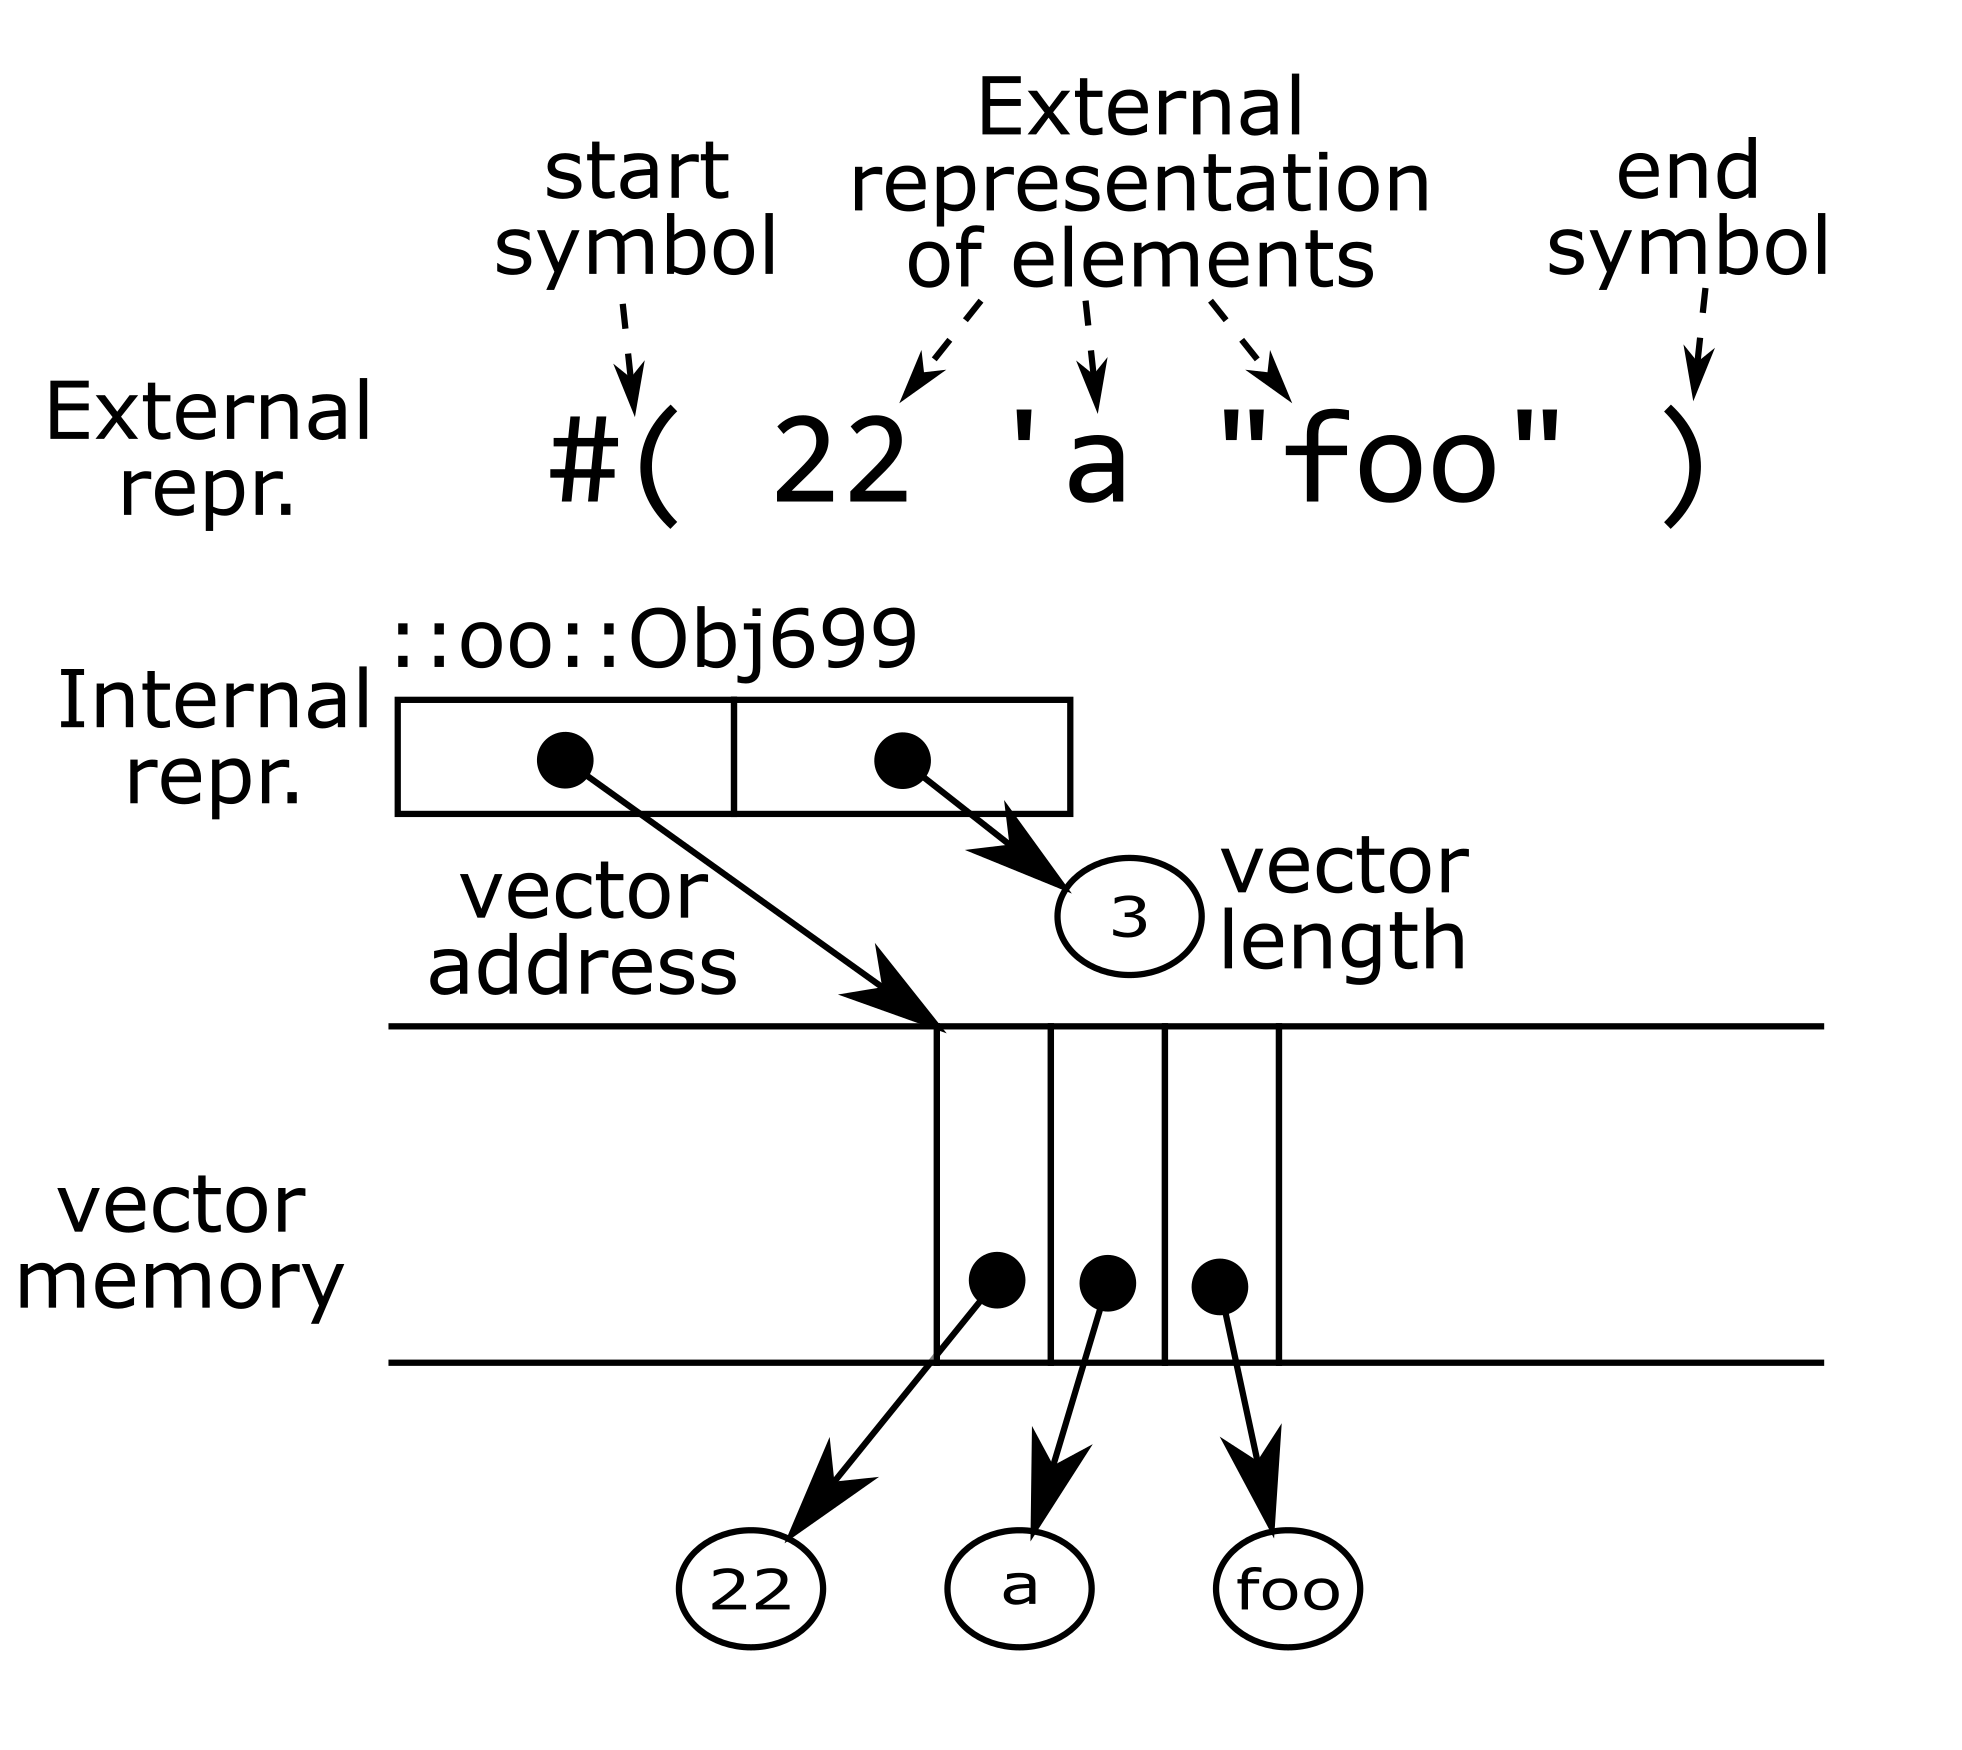
\includegraphics{images/vector-representation.png}

The \texttt{parse} procedure takes in the input buffer character by character, matching each character against a fitting external representation. When done, it creates a ConsTcl object, which is the internal representation of an expression. The object can then be passed to the evaluator.


Given a string, \texttt{parse} fills the input buffer. It then parses the input and produces the internal representation of an expression.


Example:

\begin{verbatim}
% ::constcl::parse "(+ 2 3)"
::oo::Obj491
\end{verbatim}


Here, \texttt{parse} parsed the external representation of a list with three elements, +, 2, and 3. It produced the expression that has an internal representation labeled \texttt{::oo::Obj491}. We will later meet procedures like \texttt{eval}, which transforms an expression into a value, and \texttt{write}, which prints a printed representation of expressions and values. Putting them together: we can see

\begin{verbatim}
% ::constcl::write ::oo::Obj491
(+ 2 3)
% ::constcl::eval ::oo::Obj491
::oo::Obj494
% ::constcl::write ::oo::Obj494
5
\end{verbatim}


Fortunately, we don't have to work at such a low level. We can use the \texttt{repl}\index{repl} instead:

\begin{verbatim}
ConsTcl> (+ 2 3)
5
\end{verbatim}


Then, parsing and evaluation and writing goes on in the background and the internal representations of expressions and values are hidden.


Anyway, here is how it really looks like. \texttt{::oo::Obj491} was just the head of the list.

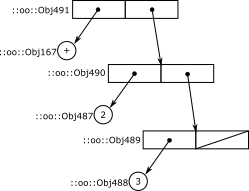
\includegraphics{images/intreplist.png}

\textbf{parse} procedure


\texttt{parse} can be called with either a string input port or a Tcl or ConsTcl string (which \texttt{parse} uses to open a string input port). Once the input port is established, \texttt{parse} leaves control to \texttt{read-expr}.

\noindent\begin{tabular}{ |p{1.5cm} p{8cm}| }
\hline
\rowcolor[HTML]{CCCCCC} \multicolumn{2}{|l|}{\bf parse (internal)} \\
inp & a Tcl string, Lisp string, or an input buffer \\
\textit{Returns:} & an expression \\
\hline
\end{tabular}
\index{parse}
\begin{lstlisting}
reg parse
 
proc ::constcl::parse {inp} {
  set c {}
  set unget {}
  if {[info object isa object $inp]} {
    if {[typeof? $inp StringInputPort] ne "#f"} {
      set port $inp
    } elseif {[typeof? $inp String] ne "#f"} {
      set port [StringInputPort new [$inp value]]
    } else {
      ::error "Unknown object [$inp show]"
    }
  } else {
    # It's a Tcl string, we hope
    set port [StringInputPort new $inp]
  }
  set oldport $::constcl::Input_port
  set ::constcl::Input_port $port
  set expr [read-expr]
  set ::constcl::Input_port $oldport
  return $expr
}
\end{lstlisting}


\textbf{make-constant} procedure


The \texttt{make-constant} helper procedure is called to set expressions to constants when read as a literal.

\index{make-constant}
\begin{lstlisting}
proc ::constcl::make-constant {val} {
  if {[pair? $val] ne "#f"} {
    $val mkconstant
    make-constant [car $val]
    make-constant [cdr $val]
  } elseif {[null? $val] ne "#f"} {
    return #NIL
  } else {
    $val mkconstant
  }
}
\end{lstlisting}


\textbf{interspace} procedure


The \texttt{interspace} helper procedure recognizes whitespace between value representations.

\index{interspace}
\begin{lstlisting}
proc ::constcl::interspace {c} {
  if {[::string is space $c] || $c eq ";"} {
      return #t
    } else {
      return #f
    }
}
\end{lstlisting}


\textbf{character-check} procedure


The \texttt{character-check} helper procedure compares a potential character constant to the valid kinds.

\noindent\begin{tabular}{ |p{1.5cm} p{8cm}| }
\hline
\rowcolor[HTML]{CCCCCC} \multicolumn{2}{|l|}{\bf character-check (internal)} \\
name & a Tcl string \\
\textit{Returns:} & a boolean \\
\hline
\end{tabular}
\index{character-check}
\begin{lstlisting}
proc ::constcl::character-check {name} {
  if {[regexp {(?i)^#\\([[:graph:]]|space|newline)$} \
      $name]} {
    return #t
  } else {
    return #f
  }
}
\end{lstlisting}
\section{read}
\label{read}
\index{read}


\textbf{read} procedure


The standard builtin \texttt{read} reads an input port the same way that \texttt{parse} takes in an input buffer. The \texttt{read-} procedures parse their input and produce ConsTcl objects.


One can pass a port to \texttt{read}, in which case \texttt{read} sets the standard input port temporarily to the provided port. If not, \texttt{read} uses the default standard input port (usually the keyboard).

\noindent\begin{tabular}{ |p{1.5cm} p{8cm}| }
\hline
\rowcolor[HTML]{CCCCCC} \multicolumn{2}{|l|}{\bf read (public)} \\
?port? & a port \\
\textit{Returns:} & an expression \\
\hline
\end{tabular}
\index{read}
\begin{lstlisting}
reg read
 
proc ::constcl::read {args} {
  set c {}
  set unget {}
  if {[llength $args]} {
    lassign $args port
  } else {
    set port $::constcl::Input_port
  }
  set oldport $::constcl::Input_port
  set ::constcl::Input_port $port
  set expr [read-expr]
  set ::constcl::Input_port $oldport
  return $expr
}
\end{lstlisting}


\textbf{read-expr} procedure


The procedure \texttt{read-expr} reads input by reading the first available character and delegating to one of the more detailed reading procedures based on that, producing an expression of any kind. A Tcl character value can be passed to it, that character will be used first before reading from the input stream. If end of file is encountered before an expression can be read in full, the procedure returns end of file (\texttt{\#EOF})\index{end of file}.

\noindent\begin{tabular}{ |p{1.5cm} p{8cm}| }
\hline
\rowcolor[HTML]{CCCCCC} \multicolumn{2}{|l|}{\bf read-expr (internal)} \\
?char? & a Tcl character \\
\textit{Returns:} & an expression or end of file \\
\hline
\end{tabular}
\index{read-expr}
\begin{lstlisting}
proc ::constcl::read-expr {args} {
  upvar c c unget unget
  if {[llength $args]} {
    lassign $args c
  } else {
    set c [readc]
  }
  set unget {}
  read-eof $c
  if {[::string is space $c] || $c eq ";"} {
    skip-ws
    read-eof $c
  }
  switch -regexp $c {
    {\"}          { read-string-expr }
    {\#}          { read-sharp }
    {\'}          { read-quoted-expr }
    {\(}          { read-pair-expr ")" }
    {\+} - {\-}   { read-plus-minus $c }
    {\,}          { read-unquoted-expr }
    {\.} {
        set x [Dot new]; set c [readc]; set x
    }
    {\:}          { read-object-expr }
    {\[}          { read-pair-expr "\]" }
    {\`}          { read-quasiquoted-expr }
    {\d}          { read-number-expr $c }
    {^$}          { return}
    {[[:graph:]]} { read-identifier-expr $c }
    default {
      read-eof $c
      ::error "unexpected character ($c)"
    }
  }
}
\end{lstlisting}


\textbf{readc} procedure


\texttt{readc} reads one character from the unget store if it isn't empty or else from the input stream. If the input stream is at end-of-file, an eof object is returned.

\noindent\begin{tabular}{ |p{1.5cm} p{8cm}| }
\hline
\rowcolor[HTML]{CCCCCC} \multicolumn{2}{|l|}{\bf readc (internal)} \\
\textit{Returns:} & a Tcl character or end of file \\
\hline
\end{tabular}
\index{readc}
\begin{lstlisting}
proc ::constcl::readc {} {
  upvar unget unget
  if {$unget ne {}} {
    set c $unget
    set unget {}
  } else {
    set c [$::constcl::Input_port get]
    if {[$::constcl::Input_port eof]} {
      return #EOF
    }
  }
  return $c
}
\end{lstlisting}


\textbf{read-find} procedure


\texttt{read-find} reads ahead through whitespace to find a given character. Returns 1 if it has found the character, and 0 if it has stopped at some other character. Returns end of file if eof is encountered.

\noindent\begin{tabular}{ |p{1.5cm} p{8cm}| }
\hline
\rowcolor[HTML]{CCCCCC} \multicolumn{2}{|l|}{\bf read-find (internal)} \\
char & a Tcl character \\
\textit{Returns:} & a Tcl truth value (1 or 0) or end of file \\
\hline
\end{tabular}
\index{read-find}
\begin{lstlisting}
proc ::constcl::read-find {char} {
  upvar c c unget unget
  while {[::string is space -strict $c]} {
    set c [readc]
    read-eof $c
    set unget $c
  }
  return [expr {$c eq $char}]
}
\end{lstlisting}


\textbf{read-end} procedure


\texttt{read-end} reads one character and returns 1 if it is an interspace character or an ending parenthesis or bracket, or end of file. Otherwise it returns 0. It ungets the character before returning.

\noindent\begin{tabular}{ |p{1.5cm} p{8cm}| }
\hline
\rowcolor[HTML]{CCCCCC} \multicolumn{2}{|l|}{\bf read-end (internal)} \\
\textit{Returns:} & a Tcl truth value (1 or 0) or end of file \\
\hline
\end{tabular}
\index{read-end}
\begin{lstlisting}
proc ::constcl::read-end {} {
  upvar c c unget unget
  set c [readc]
  if {[interspace $c] ne "#f" || $c in {) ]} || $c eq "#EOF"} {
    set unget $c
    return 1
  } else {
    set unget $c
    return 0
  }
}
\end{lstlisting}


\textbf{skip-ws} procedure


\texttt{skip-ws} skips whitespace and comments (the \texttt{;} to end of line kind). Uses the shared \emph{c} variable. It leaves the first character not to be skipped in \emph{c}.

\noindent\begin{tabular}{ |p{1.5cm} p{8cm}| }
\hline
\rowcolor[HTML]{CCCCCC} \multicolumn{2}{|l|}{\bf skip-ws (internal)} \\
\textit{Returns:} & nothing \\
\hline
\end{tabular}
\index{skip-ws}
\begin{lstlisting}
proc ::constcl::skip-ws {} {
  upvar c c unget unget
  while true {
    switch -regexp $c {
      {[[:space:]]} {
        set c [readc]
      }
      {;} {
        while {$c ne "\n" && $c ne "#EOF"}  {
          set c [readc]
        }
      }
      default {
        set unget $c
        return
      }
    }
  }
}
\end{lstlisting}


\textbf{read-eof} procedure


\texttt{read-eof} checks a number of presumed characters for possible end-of-file objects. If it finds one, it returns \emph{from its caller} with the EOF value.

\noindent\begin{tabular}{ |p{1.5cm} p{8cm}| }
\hline
\rowcolor[HTML]{CCCCCC} \multicolumn{2}{|l|}{\bf read-eof (internal)} \\
chars & some characters \\
\hline
\end{tabular}
\index{read-eof}
\begin{lstlisting}
proc ::constcl::read-eof {args} {
  set chars $args
  foreach char $chars {
    if {$char eq "#EOF"} {
      return -level 1 -code return #EOF
    }
  }
}
\end{lstlisting}


\textbf{read-string-expr} procedure


\texttt{read-string-expr} is activated by \texttt{read-expr} when it reads a double quote. It collects characters until it reaches another (unescaped) double quote. It then returns a string expression--an immutable String (see page \pageref{strings}) object.

\noindent\begin{tabular}{ |p{1.5cm} p{8cm}| }
\hline
\rowcolor[HTML]{CCCCCC} \multicolumn{2}{|l|}{\bf read-string-expr (internal)} \\
\textit{Returns:} & a string or end of file \\
\hline
\end{tabular}
\index{read-string-expr}
\begin{lstlisting}
proc ::constcl::read-string-expr {} {
  upvar c c unget unget
  set str {}
  set c [readc]
  read-eof $c
  while {$c ne "\"" && $c ne "#EOF"} {
    if {$c eq "\\"} {
      ::append str $c
      set c [readc]
    }
    ::append str $c
    set c [readc]
  }
  if {$c eq "#EOF"} {
    error "bad string (no ending double quote)"
  }
  set c [readc]
  set expr [MkString $str]
  read-eof $expr
  $expr mkconstant
  return $expr
}
\end{lstlisting}


\textbf{read-sharp} procedure


\texttt{read-sharp} is activated by \texttt{read-expr} when it reads a sharp sign (\texttt{\#}). It in turn either delegates to the vector reader or the character reader, or returns boolean literals.

\noindent\begin{tabular}{ |p{1.5cm} p{8cm}| }
\hline
\rowcolor[HTML]{CCCCCC} \multicolumn{2}{|l|}{\bf read-sharp (internal)} \\
\textit{Returns:} & a vector, boolean, or character value or end of file \\
\hline
\end{tabular}
\index{read-sharp}
\begin{lstlisting}
proc ::constcl::read-sharp {} {
  upvar c c unget unget
  set unget {}
  set c [readc]
  read-eof $c
  switch $c {
    (    { set n [read-vector-expr] }
    t    { if {[read-end]} {set n #t} }
    f    { if {[read-end]} {set n #f} }
    "\\" { set n [read-character-expr] }
    default {
      ::error "Illegal #-literal: #$c"
    }
  }
  return $n
}
\end{lstlisting}


\textbf{read-vector-expr} procedure


\texttt{read-vector-expr} is activated by \texttt{read-sharp} and reads a number of expressions until it finds an ending parenthesis. It produces a vector expression and returns a Vector (see page \pageref{vectors}) object.

\noindent\begin{tabular}{ |p{1.5cm} p{8cm}| }
\hline
\rowcolor[HTML]{CCCCCC} \multicolumn{2}{|l|}{\bf read-vector-expr (internal)} \\
\textit{Returns:} & a vector or end of file \\
\hline
\end{tabular}
\index{read-vector-expr}
\begin{lstlisting}
proc ::constcl::read-vector-expr {} {
  upvar c c unget unget
  set res {}
  set last {}
  set c [readc]
  while {$c ne "#EOF" && $c ne ")"} {
    set e [cons [read-expr $c] #NIL]
    if {$res eq {}} {
      set res $e
      set last $e
    } else {
      set-cdr! $last $e
      set last $e
    }
    skip-ws
    read-eof $c
  }
  if {$c ne ")"} {
    ::error "Missing right paren. ($c)."
  }
  set expr [MkVector $res]
  read-eof $expr
  $expr mkconstant
  return $expr
}
\end{lstlisting}


\textbf{read-character-expr} procedure


\texttt{read-character-expr} reads input, producing a character and returning a Char (see page \pageref{characters}) object.

\noindent\begin{tabular}{ |p{1.5cm} p{8cm}| }
\hline
\rowcolor[HTML]{CCCCCC} \multicolumn{2}{|l|}{\bf read-character-expr (internal)} \\
\textit{Returns:} & a character or end of file \\
\hline
\end{tabular}
\index{read-character-expr}
\begin{lstlisting}
proc ::constcl::read-character-expr {} {
  upvar c c unget unget
  set name "#\\"
  set c [readc]
  read-eof $c
  while {$c ni {) ]} && [::string is graph $c] && $c ne "#EOF"} {
    ::append name $c
    set c [readc]
  }
  check {character-check $name} {
      Invalid character constant $name
  }
  set expr [MkChar $name]
  read-eof $expr
  return $expr
}
\end{lstlisting}


\textbf{read-quoted-expr} procedure


\texttt{read-quoted-expr} is activated by \texttt{read-expr} when reading a single quote ('). It then reads an entire expression beyond that, returning it wrapped in a list with \texttt{quote}. The quoted expression is made constant.

\noindent\begin{tabular}{ |p{1.5cm} p{8cm}| }
\hline
\rowcolor[HTML]{CCCCCC} \multicolumn{2}{|l|}{\bf read-quoted-expr (internal)} \\
\textit{Returns:} & an expression wrapped in the quote symbol or end of file \\
\hline
\end{tabular}
\index{read-quoted-expr}
\begin{lstlisting}
proc ::constcl::read-quoted-expr {} {
  upvar c c unget unget
  set unget {}
  set expr [read-expr]
  read-eof $expr
  make-constant $expr
  return [list [S quote] $expr]
}
\end{lstlisting}


\textbf{read-pair-expr} procedure


The \texttt{read-pair-expr} procedure reads everything between two matching parentheses, or, as the case might be, brackets. It produces either an empty list, or a possibly recursive structure of Pair (see page \pageref{pairs-and-lists}) objects, either a proper list (one that ends in \texttt{\#NIL}), or an improper one (one that has an atom as its last member).

\noindent\begin{tabular}{ |p{1.5cm} p{8cm}| }
\hline
\rowcolor[HTML]{CCCCCC} \multicolumn{2}{|l|}{\bf read-pair-expr (internal)} \\
char & the terminating paren or bracket \\
\textit{Returns:} & a structure of pair expressions or end of file \\
\hline
\end{tabular}
\index{read-pair-expr}
\begin{lstlisting}
proc ::constcl::read-pair-expr {char} {
  upvar c c unget unget
  set unget {}
  set expr [read-pair $char]
  read-eof $expr
  if {$c ne $char} {
    if {$char eq ")"} {
      ::error \
        "Missing right paren. ($c)."
    } else {
      ::error \
        "Missing right bracket ($c)."
    }
  } else {
    set unget {}
    set c [readc]
  }
  return $expr
}
\end{lstlisting}


\texttt{read-pair} is a helper procedure that does the heavy lifting in reading a pair structure. First it checks if the list is empty, returning \texttt{\#NIL} in that case. Otherwise it reads the first element in the list and then repeatedly the rest of them. If it reads a Dot object, the following element to be read is the tail end of an improper list. When \texttt{read-pair} has reached the ending parenthesis or bracket, it conses up the elements starting from the last, and returns the head of the list.

\index{read-pair}
\begin{lstlisting}
proc ::constcl::read-pair {char} {
  upvar c c unget unget
  set c [readc]
  read-eof $c
  if {[read-find $char]} {
    # read right paren/brack
    #set c [readc]
    return #NIL
  }
  set a [read-expr $c]
  set res $a
  skip-ws
  set prev #NIL
  while {![read-find $char]} {
    set x [read-expr $c]
    skip-ws
    read-eof $c
    if {[dot? $x] ne "#f"} {
      set prev [read-expr $c]
      skip-ws
      read-eof $c
    } else {
      lappend res $x
    }
    if {[llength $res] > 99} break
  }
  # read right paren/brack
  foreach r [lreverse $res] {
    set prev [cons $r $prev]
  }
  return $prev
}
\end{lstlisting}


\textbf{read-plus-minus} procedure


\texttt{read-plus-minus} is called when a plus or minus is found in the input stream. If the next character is a digit, it delegates to the number reader. Otherwise, it returns a \texttt{+} or \texttt{-} symbol.

\noindent\begin{tabular}{ |p{1.5cm} p{8cm}| }
\hline
\rowcolor[HTML]{CCCCCC} \multicolumn{2}{|l|}{\bf read-plus-minus (internal)} \\
\textit{Returns:} & either the symbols + or - or a number or end of file \\
\hline
\end{tabular}
\index{read-plus-minus}
\begin{lstlisting}
proc ::constcl::read-plus-minus {char} {
  upvar c c unget unget
  set unget {}
  set c [readc]
  read-eof $c
  if {[::string is digit -strict $c]} {
    set n [read-number-expr $c]
    read-eof $n
    if {$char eq "-"} {
      set n [- $n]
    }
    return $n
  } elseif {[::string is space -strict $c] ||
      $c in {) ]}} {
    if {$char eq "+"} {
      return [S "+"]
    } else {
      return [S "-"]
    }
  } else {
    set n [read-identifier-expr $char $c]
    read-eof $n
    return $n
  }
}
\end{lstlisting}


\textbf{read-number-expr} procedure


\texttt{read-number-expr} reads numerical input, both integers and floating point numbers. It actually takes in anything that starts out like a number and stops at whitespace or an ending parenthesis or bracket, and then it accepts or rejects the input by comparing it to a Tcl double. It returns a Number (see page \pageref{numbers}) object.

\noindent\begin{tabular}{ |p{1.5cm} p{8cm}| }
\hline
\rowcolor[HTML]{CCCCCC} \multicolumn{2}{|l|}{\bf read-number-expr (internal)} \\
?char? & a Tcl character \\
\textit{Returns:} & a number or end of file \\
\hline
\end{tabular}
\index{read-number-expr}
\begin{lstlisting}
proc ::constcl::read-number-expr {args} {
  upvar c c unget unget
  set unget {}
  if {[llength $args]} {
    lassign $args c
  } else {
    set c [readc]
  }
  read-eof $c
  while {[interspace $c] ne "#t" && $c ne "#EOF" &&
      $c ni {) ]}} {
    ::append num $c
    set c [readc]
  }
  set unget $c
  check {::string is double -strict $num} {
      Invalid numeric constant $num
  }
  set expr [N $num]
  return $expr
}
\end{lstlisting}


\textbf{read-unquoted-expr} procedure


When a comma is found in the input stream, \texttt{read-unquoted-expr} is activated. If it reads an at-sign (\texttt{@}) it selects the symbol \texttt{unquote-splicing}, otherwise it selects the symbol \texttt{unquote}. Then it reads an entire expression and returns it wrapped in the selected symbol. Both of these expressions are only suppposed to occur inside a quasiquoted expression.

\noindent\begin{tabular}{ |p{1.5cm} p{8cm}| }
\hline
\rowcolor[HTML]{CCCCCC} \multicolumn{2}{|l|}{\bf read-unquoted-expr (internal)} \\
\textit{Returns:} & an expr. wr. in the unquote/-splicing symbol or end of file \\
\hline
\end{tabular}
\index{read-unquoted-expr}
\begin{lstlisting}
proc ::constcl::read-unquoted-expr {} {
  upvar c c unget unget
  set unget {}
  set c [readc]
  read-eof $c
  if {$c eq "@"} {
    set symbol "unquote-splicing"
    set expr [read-expr]
  } else {
    set symbol "unquote"
    set expr [read-expr $c]
  }
  read-eof $expr
  return [list [S $symbol] $expr]
}
\end{lstlisting}


\textbf{read-quasiquoted-expr} procedure


\texttt{read-quasiquoted-expr} is activated when there is a backquote (\texttt{`}) in the input stream. It reads an entire expression and returns it wrapped in \texttt{quasiquote}.

\noindent\begin{tabular}{ |p{1.5cm} p{8cm}| }
\hline
\rowcolor[HTML]{CCCCCC} \multicolumn{2}{|l|}{\bf read-quasiquoted-expr (internal)} \\
\textit{Returns:} & an expr. wr. in the quasiquote symbol or end of file \\
\hline
\end{tabular}
\index{read-quasiquoted-expr}
\begin{lstlisting}
proc ::constcl::read-quasiquoted-expr {} {
  upvar c c unget unget
  set unget {}
  set expr [read-expr]
  skip-ws
  read-eof $expr
  make-constant $expr
  return [list [S quasiquote] $expr]
}
\end{lstlisting}


\textbf{read-identifier-expr} procedure


\texttt{read-identifier-expr} is activated for 'anything else', and takes in characters until it finds whitespace or an ending parenthesis or bracket. It checks the input against the rules for identifiers, accepting or rejecting it with an error message. It returns a Symbol (see page \pageref{symbols}) object.

\noindent\begin{tabular}{ |p{1.5cm} p{8cm}| }
\hline
\rowcolor[HTML]{CCCCCC} \multicolumn{2}{|l|}{\bf read-identifier-expr (internal)} \\
?chars? & some Tcl characters \\
\textit{Returns:} & a symbol or end of file \\
\hline
\end{tabular}
\index{read-identifier-expr}
\begin{lstlisting}
proc ::constcl::read-identifier-expr {args} {
  upvar c c unget unget
  set unget {}
  if {[llength $args]} {
    set c [join $args {}]
  } else {
    set c [readc]
  }
  read-eof $c
  set name {}
  while {[::string is graph -strict $c]} {
    if {$c eq "#EOF" || $c in {) \]}} {
      break
    }
    ::append name $c
    set c [readc]
    # do not check for EOF here
  }
  if {$c ne "#EOF"} {
    set unget $c
  }
  read-eof $name
  # idcheck throws error if invalid identifier
  idcheck $name
  return [S $name]
}
\end{lstlisting}


\textbf{read-object-expr} procedure


A non-standard extension, \texttt{read-object-expr} reads a ConsTcl object of any kind and passes its name along.

\noindent\begin{tabular}{ |p{1.5cm} p{8cm}| }
\hline
\rowcolor[HTML]{CCCCCC} \multicolumn{2}{|l|}{\bf read-object-expr (internal)} \\
\textit{Returns:} & a ConsTcl object or end of file \\
\hline
\end{tabular}
\index{read-object-expr}
\begin{lstlisting}
proc ::constcl::read-object-expr {} {
  upvar c c unget unget
  # first colon has already been read
  foreach ch [split ":oo::Obj" {}] {
    set c [readc]
    read-eof $c
    if {$c ne $ch} {
      error "bad object name"
    }
  }
  set res "::oo::Obj"
  set c [readc]
  read-eof $c
  while {[::string is digit $c]} {
    ::append res $c
    set c [readc]
    read-eof $c
  }
  set unget $c
  return $res
}
\end{lstlisting}
\chapter{Evaluation}
\label{evaluation}


The second thing an interpreter must be able to do is to reduce expressions to their \emph{normal form}, or \emph{evaluate}\index{eval}\index{evaluator} them. As an example, 2 + 6 and 8 are two expressions that have the same value, but the latter is in normal form (can't be reduced further) and the former is not.

\section{Syntactic forms}
\label{syntactic-forms}
\index{syntactic forms}


There are nine diffent forms or classes of expressions in Lisp. The evaluator recognizes each one by its internal representation and chooses the appropriate process to evaluate them. The nine forms will be described in the following sections.



\textbf{eval} procedure


The heart of the Lisp interpreter, \texttt{eval} takes a Lisp expression and processes it according to its syntactic form.


\texttt{eval} also does two kinds of rewriting of expressions: 1) \emph{macro expansion} on a non-atomic expression into a more concrete expression. See the part about macros (see page \pageref{macros}) below, and 2) resolving \emph{local defines}, acting on expressions of the form K{(begin (define \ldots } when in a local environment. See the part about resolving local defines (see page \pageref{resolving-local-defines}).

\noindent\begin{tabular}{ |p{1.5cm} p{8cm}| }
\hline
\rowcolor[HTML]{CCCCCC} \multicolumn{2}{|l|}{\bf eval (public)} \\
expr & an expression \\
env & an environment \\
\textit{Returns:} & a Lisp value \\
\hline
\end{tabular}
\index{eval}
\begin{lstlisting}
reg eval
 
proc ::constcl::eval \
  {expr {env ::constcl::global_env}} {
  if {[symbol? $expr] ne "#f"} {
    lookup $expr $env
  } elseif {[null? $expr] ne "#f" ||
    [atom? $expr] ne "#f"} {
    set expr
  } else {
    while {[[car $expr] name] in
      $::constcl::macrolist} {
      set expr [expand-macro $expr $env]
    }
    set op [car $expr]
    set args [cdr $expr]
    if {$env ne "::constcl::global_env" &&
      [$op name] eq "begin" &&
      ([pair? [car $args]] ne "#f" &&
      [[caar $args] name] eq "define")} {
      set expr [resolve-local-defines $args]
      set op [car $expr]
      set args [cdr $expr]
    }
    switch [$op name] {
      quote {
        car $args
      }
      if {
        if {[eval [car $args] $env] ne "#f"} \
          {eval [cadr $args] $env} \
          {eval [caddr $args] $env}
      }
      begin {
        /begin $args $env
      }
      define {
        /define [car $args] [
          eval [cadr $args] $env] $env
      }
      set! {
        /set! [car $args] [
          eval [cadr $args] $env] $env 
      }
      lambda {
        /lambda [car $args] [
          cdr $args] $env
      }
      default {
        invoke [eval $op $env] [
          eval-list $args $env]
      }
    }
  }
}
\end{lstlisting}
\subsection{Variable reference}
\label{variable-reference}
\index{variable reference}


\emph{Example: \texttt{r} => 10 (a symbol \texttt{r} is evaluated to 10)}


A variable\index{variable}\index{variable reference} is an identifier (symbol) bound to a location in the environment. If an expression consists of an identifier it is evaluated to the value stored in that location. This is handled by the helper procedure \texttt{lookup}. It searches the environment chain for the identifier, and returns the value stored in the location it is bound to. It is an error to do lookup on an unbound symbol.


\textbf{lookup} procedure

\noindent\begin{tabular}{ |p{1.5cm} p{8cm}| }
\hline
\rowcolor[HTML]{CCCCCC} \multicolumn{2}{|l|}{\bf lookup (internal)} \\
sym & a symbol \\
env & an environment \\
\textit{Returns:} & a Lisp value \\
\hline
\end{tabular}
\index{lookup}
\begin{lstlisting}
proc ::constcl::lookup {sym env} {
  [$env find $sym] get $sym
}
\end{lstlisting}
\subsection{Constant literal}
\label{constant-literal}
\index{constant literal}


\emph{Example: \texttt{99} => 99 (a number evaluates to itself)}


Not just numbers\index{constant literal} but booleans, characters, strings, and vectors evaluate to themselves, to their innate value. Because of this, they are called autoquoting types (see next paragraph).

\subsection{Quotation}
\label{quotation}
\index{quotation}


\emph{Example: \texttt{(quote r)} => \texttt{r} (quotation makes the symbol evaluate to itself, like a constant)}


According to the rules of variable reference, a symbol evaluates to its stored value. Well, sometimes one wishes to use the symbol itself as a value. That is what quotation\index{quotation} is for. \texttt{(quote x)} evaluates to the symbol \texttt{x} itself and not to any value that might be stored under it. This is so common that there is a shorthand notation for it: \texttt{'x} is interpreted as \texttt{(quote x)} by the Lisp reader.

\subsection{Conditional}
\label{conditional}
\index{conditional}


\emph{Example: \texttt{(if (> 99 100) (* 2 2) (+ 2 4))} => 6}


The conditional\index{conditional} form \texttt{if} evaluates a Lisp list of three expressions. The first, the \emph{condition}, is evaluated first. If it evaluates to anything other than \texttt{\#f} (false), the second expression (the \emph{consequent}) is evaluated and the value returned. Otherwise, the third expression (the \emph{alternate}) is evaluated and the value returned. One of the two latter expressions will be evaluated, and the other will remain unevaluated.


\textbf{/if} procedure

\noindent\begin{tabular}{ |p{1.5cm} p{8cm}| }
\hline
\rowcolor[HTML]{CCCCCC} \multicolumn{2}{|l|}{\bf /if (internal)} \\
condition & an expression \\
consequent & an expression \\
alternate & an expression \\
\textit{Returns:} & a Lisp value \\
\hline
\end{tabular}
\index{/if}
\begin{lstlisting}
proc ::constcl::/if {cond conseq altern} {
  if {[uplevel $cond] ne "#f"} {
    uplevel $conseq
  } {
    uplevel $altern
  }
}
\end{lstlisting}
\subsection{Sequence}
\label{sequence}
\index{sequence}


\emph{Example: \texttt{(begin (define r 10) (* r r))} => 100}


When expressions are evaluated in sequence\index{sequence}, the order is important for two reasons. If the expressions have any side effects, they happen in the same order of sequence. Also, if expressions are part of a pipeline of calculations, then they need to be processed in the order of that pipeline. The \texttt{/begin} helper procedure takes a Lisp list of expressions and evaluates them in sequence, returning the value of the last one.


\textbf{/begin} procedure

\noindent\begin{tabular}{ |p{1.5cm} p{8cm}| }
\hline
\rowcolor[HTML]{CCCCCC} \multicolumn{2}{|l|}{\bf /begin (internal)} \\
exps & a Lisp list of expressions \\
env & an environment \\
\textit{Returns:} & a Lisp value \\
\hline
\end{tabular}
\index{/begin}
\begin{lstlisting}
proc ::constcl::/begin {exps env} {
  /if {pair? $exps} {
    /if {pair? [cdr $exps]} {
      eval [car $exps] $env
      return [/begin [cdr $exps] $env]
    } {
      return [eval [car $exps] $env]
    }
  } {
    return #NIL
  }
}
\end{lstlisting}
\subsection{Definition}
\label{definition}
\index{definition}


\emph{Example: \texttt{(define r 10)} => \ldots  (a definition doesn't evaluate to anything)}


We've already seen the relationship between symbols and values. Through (variable) definition\index{variable definition}\index{definition}, a symbol is bound to a value (or rather to the location the value is in), creating a variable. The \texttt{/define} helper procedure adds a variable to the current environment. It first checks that the symbol name is a valid identifier, then it updates the environment with the new binding.


\textbf{/define} procedure

\noindent\begin{tabular}{ |p{1.5cm} p{8cm}| }
\hline
\rowcolor[HTML]{CCCCCC} \multicolumn{2}{|l|}{\bf /define (internal)} \\
sym & a symbol \\
val & a Lisp value \\
env & an environment \\
\textit{Returns:} & nothing \\
\hline
\end{tabular}
\index{/define}
\begin{lstlisting}
proc ::constcl::/define {sym val env} {
  varcheck [idcheck [$sym name]]
  $env set $sym $val
  return
}
\end{lstlisting}
\subsection{Assignment}
\label{assignment}
\index{assignment}


\emph{Example: \texttt{(set! r 20)} => 20 (\texttt{r} is a bound symbol, so it's allowed to assign to it)}


Once a variable has been created, the value at the location it is bound to can be changed (hence the name "variable", something that can be modified). The process is called assignment\index{assignment}. The \texttt{/set!} helper does assignment: it modifies an existing variable that is bound somewhere in the environment chain. It finds the variable's environment and updates the binding. It returns the value, so calls to \texttt{set!} can be chained: \texttt{(set! foo (set! bar 99))} sets both variables to 99. By Scheme convention, procedures that modify variables have "!" at the end of their name.


\textbf{/set!} procedure

\noindent\begin{tabular}{ |p{1.5cm} p{8cm}| }
\hline
\rowcolor[HTML]{CCCCCC} \multicolumn{2}{|l|}{\bf /set! (internal)} \\
var & a bound symbol \\
val & a Lisp value \\
env & an environment \\
\textit{Returns:} & a Lisp value \\
\hline
\end{tabular}
\index{/set!}
\begin{lstlisting}
proc ::constcl::/set! {var val env} {
  [$env find $var] set $var $val
  set val
}
\end{lstlisting}
\subsection{Procedure definition}
\label{procedure-definition}
\index{procedure definition}


\emph{Example: \texttt{(lambda (r) (* r r))} => \texttt{::oo::Obj3601} (it will be a different object each time)}


In Lisp, procedures are values just like numbers or characters. They can be defined\index{procedure definition} as the value of a symbol, passed to other procedures, and returned from procedures. One diffence from most values is that procedures need to be defined. Two questions must answered: what is the procedure meant to do? The code that does that will form the body of the procedure. Also, what, if any, items of data will have to be provided to the procedure to make it possible to calculate its result?


As an example, imagine that we want to have a procedure that calculates the square (\texttt{x * x}) of a given number. In Lisp, expressions are written with the operator first and then the operands: \texttt{(* x x)}. That is the body of the procedure. Now, what data will we have to provide to the procedure to make it work? A value stored in the variable \texttt{x} will do. It's only a single variable, but by custom we need to put it in a list: \texttt{(x)}. The operator that defines procedures is called \texttt{lambda}\index{lambda}, and we define the function with \texttt{(lambda (x) (* x x))}.


One more step is needed before we can use the procedure. It must have a name. We could define it like this: \texttt{(define square (lambda (x) (* x x)))} but there is actually a shortcut notation for it: \texttt{(define (square x) (* x x))}.


Now, \texttt{square} is pretty tame. How about the \texttt{hypotenuse} procedure? \texttt{(define (hypotenuse a b) (sqrt (+ (square a) (square b))))}. It calculates the square root of the sum of two squares.


Under the hood, the helper \texttt{/lambda} makes a Procedure (see page \pageref{control}) object. First it needs to convert the Lisp list \texttt{body}. It is packed inside a \texttt{begin} if it has more than one expression (\texttt{S begin} stands for "the symbol begin".), and taken out of its list if not. The Lisp list \texttt{formals} is passed on as it is.

\subsubsection{Scheme formals lists: an aside}
\label{scheme-formals-lists:-an-aside}

A Scheme formals list\index{formals list} is either:

\begin{itemize}
\item  An \emph{empty list}, \texttt{()}, meaning that no arguments are accepted,
\item  A \emph{proper list}, \texttt{(a b c)}, meaning it accepts three arguments, one in each symbol,
\item  A \emph{symbol}, \texttt{a}, meaning that all arguments go into \texttt{a}, or
\item  A \emph{dotted list}, \texttt{(a b . c)}, meaning that two arguments go into \texttt{a} and \texttt{b}, and the rest into \texttt{c}.
\end{itemize}

\textbf{/lambda} procedure

\noindent\begin{tabular}{ |p{1.5cm} p{8cm}| }
\hline
\rowcolor[HTML]{CCCCCC} \multicolumn{2}{|l|}{\bf /lambda (internal)} \\
formals & a Scheme formals list \\
body & a Lisp list of expressions \\
env & an environment \\
\textit{Returns:} & a procedure \\
\hline
\end{tabular}
\index{/lambda}
\begin{lstlisting}
proc ::constcl::/lambda {formals body env} {
  if {[[length $body] value] > 1} {
    set body [cons [S begin] $body]
  } else {
    set body [car $body]
  }
  return [MkProcedure $formals $body $env]
}
\end{lstlisting}
\subsection{Procedure call}
\label{procedure-call}
\index{procedure call}


\emph{Example: \texttt{(+ 1 6)} => 7}


Once we have procedures, we can call\index{procedure call} them to have their calculations performed and yield results. The procedure name is put in the operator position at the front of a list, and the operands follow in the rest of the list. Our \texttt{square} procedure would be called for instance like this: \texttt{(square 11)}, and it will return 121.


\texttt{invoke} arranges for a procedure to be called with each of the values in the \emph{argument list} (the list of operands). It checks if pr really is a procedure, and determines whether to call pr as an object or as a Tcl command.


\textbf{invoke} procedure

\noindent\begin{tabular}{ |p{1.5cm} p{8cm}| }
\hline
\rowcolor[HTML]{CCCCCC} \multicolumn{2}{|l|}{\bf invoke (internal)} \\
pr & a procedure \\
vals & a Lisp list of Lisp values \\
\textit{Returns:} & what pr returns \\
\hline
\end{tabular}
\index{invoke}
\begin{lstlisting}
proc ::constcl::invoke {pr vals} {
  check {procedure? $pr} {
    PROCEDURE expected\n([$pr show] val ...)
  }
  if {[info object isa object $pr]} {
    $pr call {*}[splitlist $vals]
  } else {
    $pr {*}[splitlist $vals]
  }
}
\end{lstlisting}


\textbf{splitlist} procedure


\texttt{splitlist} converts a Lisp list to a Tcl list with Lisp objects.

\noindent\begin{tabular}{ |p{1.5cm} p{8cm}| }
\hline
\rowcolor[HTML]{CCCCCC} \multicolumn{2}{|l|}{\bf splitlist (internal)} \\
vals & a Lisp list of Lisp values \\
\textit{Returns:} & a Tcl list of Lisp values \\
\hline
\end{tabular}
\index{splitlist}
\begin{lstlisting}
proc ::constcl::splitlist {vals} {
  set result {}
  while {[pair? $vals] ne "#f"} {
    lappend result [car $vals]
    set vals [cdr $vals]
  }
  return $result
}
\end{lstlisting}


\textbf{eval-list} procedure


\texttt{eval-list} successively evaluates the elements of a Lisp list and returns the collected results as a Lisp list.

\noindent\begin{tabular}{ |p{1.5cm} p{8cm}| }
\hline
\rowcolor[HTML]{CCCCCC} \multicolumn{2}{|l|}{\bf eval-list (internal)} \\
exps & a Lisp list of expressions \\
env & an environment \\
\textit{Returns:} & a Lisp list of Lisp values \\
\hline
\end{tabular}
\index{eval-list}
\begin{lstlisting}
proc ::constcl::eval-list {exps env} {
  # don't convert to /if, it breaks (fact 100)
  if {[pair? $exps] ne "#f"} {
    return [cons [eval [car $exps] $env] \
      [eval-list [cdr $exps] $env]]
  } {
    return #NIL
  }
}
\end{lstlisting}
\section{Macros}
\label{macros}
\index{macros}


\textbf{expand-macro} procedure


Macros that allow concise, abstract expressions that are automatically rewritten into other, more concrete but also more verbose expressions is one of Lisp's strong points. This interpreter does macro expansion, but the user can't define new macros--the ones available are hardcoded in the code below.


\texttt{expand-macro} takes an expression and an environment as a parameter. First, the operator (\texttt{op}) and operands (\texttt{args}) are extracted to check if expansion is necessary (the operator \texttt{car}, for historical reasons, stands for the first element of a list, while \texttt{cdr} stands for the rest of the elements after the first in a list). If the operator is the symbol \texttt{define} and the first of the operands is something other than a Pair, then expansion is unnecessary and the procedure returns with a code to break the while loop in \texttt{eval}.


The operator's symbol name is then used to select the right expansion procedure, and the whole expression and the environment is passed to it. In the end, the expanded expression is passed back to \texttt{eval}.

\noindent\begin{tabular}{ |p{1.5cm} p{8cm}| }
\hline
\rowcolor[HTML]{CCCCCC} \multicolumn{2}{|l|}{\bf expand-macro (internal)} \\
expr & an expression \\
env & an environment \\
\textit{Returns:} & an expression \\
\hline
\end{tabular}
\index{expand-macro}
\begin{lstlisting}
proc ::constcl::expand-macro {expr env} {
  set op [car $expr]
  set args [cdr $expr]
  if {[$op name] eq "define" &&
      [pair? [car $args]] eq "#f"} {
    return -code break
  }
  return [expand-[$op name] $expr $env]
}
\end{lstlisting}


\textbf{expand-and} procedure


\texttt{expand-and} expands the \texttt{and} macro. It returns a \texttt{begin}-expression if the macro has 0 or 1 elements, and a nested \texttt{if} construct otherwise.

\noindent\begin{tabular}{ |p{1.5cm} p{8cm}| }
\hline
\rowcolor[HTML]{CCCCCC} \multicolumn{2}{|l|}{\bf expand-and (internal)} \\
expr & an expression \\
env & an environment \\
\textit{Returns:} & an expression \\
\hline
\end{tabular}
\index{expand-and}
\begin{lstlisting}
regmacro and
 
proc ::constcl::expand-and {expr env} {
  set tail [cdr $expr]
  if {[[length $tail] numval] == 0} {
    list [S begin] #t
  } elseif {[[length $tail] numval] == 1} {
    cons [S begin] $tail
  } else {
    do-and $tail #t $env
  }
}
\end{lstlisting}


\textbf{do-and} procedure


\texttt{do-and} is called recursively for every argument of \texttt{expand-or} if there are more than one.

\subsubsection{Quasiquote: an aside}
\label{quasiquote:-an-aside}


In this and many other macro expanders I use a quasiquote\index{quasiquote} construct to lay out how the macro is to be expanded. A quasiquote starts with a backquote (\texttt{`}) instead of the single quote that precedes regular quoted material. A quasiquote allows for "unquoting" of selected parts: this is notated with a comma (\texttt{,}). \texttt{`(foo ,bar baz)} is very nearly the same as \texttt{('foo bar 'baz)}. In both cases \texttt{foo} and \texttt{baz} are constants while \texttt{bar} is a variable which will be evaluated. Like in \texttt{do-and} here, a quasiquote serves well as a templating mechanism. The variables in the quasiquote need to be a part of the environment in which the quasiquote is expanded: I use \texttt{/define} to bind them in a temporary environment.

\noindent\begin{tabular}{ |p{1.5cm} p{8cm}| }
\hline
\rowcolor[HTML]{CCCCCC} \multicolumn{2}{|l|}{\bf do-and (internal)} \\
tail & an expression tail \\
prev & an expression \\
env & an environment \\
\textit{Returns:} & an expression \\
\hline
\end{tabular}
\index{do-and}
\begin{lstlisting}
proc ::constcl::do-and {tail prev env} {
  if {[null? $tail] ne "#f"} {
    return $prev
  } else {
    set env [Environment new #NIL {} $env]
    /define [S first] [car $tail] $env
    /define [S rest] [do-and [cdr $tail] \
        [car $tail] $env] $env
    set qq "`(if ,first ,rest #f)"
    set expr [expand-quasiquote [parse $qq] $env]
    $env destroy
    return $expr
  }
}
\end{lstlisting}


\textbf{expand-case} procedure


The body of the \texttt{case} form consists of a key-expression and a number of clauses. Each clause has a list of values and a body. If the key-expression evaluates to a value that occurs in one of the value-lists (considered in order), that clause's body is evaluated and all other clauses are ignored.


The \texttt{case} macro is expanded by \texttt{expand-case}. It expands to \texttt{'()} if there are no clauses (left), and to nested \texttt{if} constructs if there are some.

\subsubsection{caar, cadr, cdar, and the rest: an aside}
\label{caar,-cadr,-cdar,-and-the-rest:-an-aside}


The \texttt{do-case} procedure uses extensions of the \texttt{car}/\texttt{cdr} operators like \texttt{caar} and \texttt{cdar}. \texttt{car}/\texttt{cdr} notation gets really powerful when combined to form operators from \texttt{caar} to \texttt{cddddr}. One can read \texttt{caar L} as "the first element of the first element of L", implying that the first element of \texttt{L} is a list. \texttt{cdar L} is "the rest of the elements of the first element of L", and \texttt{cadr L} is "the first element of the rest of the elements of L" or in layman's terms, the second element of L.

\noindent\begin{tabular}{ |p{1.5cm} p{8cm}| }
\hline
\rowcolor[HTML]{CCCCCC} \multicolumn{2}{|l|}{\bf expand-case (internal)} \\
expr & an expression \\
env & an environment \\
\textit{Returns:} & an expression \\
\hline
\end{tabular}
\index{expand-case}
\begin{lstlisting}
regmacro case
 
proc ::constcl::expand-case {expr env} {
  set tail [cdr $expr]
  do-case [car $tail] [cdr $tail] $env
}
 
proc ::constcl::do-case {keyexpr clauses env} {
  if {[null? $clauses] ne "#f"} {
    return [parse "'()"]
  } else {
    set keyl [caar $clauses]
    set body [cdar $clauses]
    set keyl [list [S memv] $keyexpr \
        [list [S quote] $keyl]]
    # if this is the last clause...
    if {[eq? [length $clauses] #1] ne "#f"} {
      # ...allow 'else' in the condition
      if {[eq? [caar $clauses] [S else]] ne "#f"} {
        set keyl #t
      }
    }
    set env [Environment new #NIL {} $env]
    /define [S keyl] $keyl $env
    /define [S body] $body $env
    /define [S rest] [
      do-case $keyexpr [cdr $clauses] $env] $env
    set qq "`(if ,keyl
               (begin ,@body)
               ,rest)"
    set expr [expand-quasiquote [parse $qq] $env]
    $env destroy
    return $expr
  }
}
\end{lstlisting}


\textbf{expand-cond} procedure


The \texttt{cond} form has a list of clauses, each with a predicate and a body. The clauses is considered in order, and if a predicate evaluates to something other than \texttt{\#f} the body is evaluated and the remaining clauses are ignored.


The \texttt{cond} macro is expanded by \texttt{expand-cond}. It expands to \texttt{'()} if there are no clauses (left), and to nested \texttt{if} constructs if there are some.

\noindent\begin{tabular}{ |p{1.5cm} p{8cm}| }
\hline
\rowcolor[HTML]{CCCCCC} \multicolumn{2}{|l|}{\bf expand-cond (internal)} \\
expr & an expression \\
env & an environment \\
\textit{Returns:} & an expression \\
\hline
\end{tabular}
\index{expand-cond}
\begin{lstlisting}
regmacro cond
 
proc ::constcl::expand-cond {expr env} {
  return [do-cond [cdr $expr] $env]
}
\end{lstlisting}


\textbf{do-cond} procedure


\texttt{do-cond} is called recursively for every clause of the \texttt{cond} form. It chops up the clause into predicate and body, stepping over any \texttt{=>} symbols in between. In the last clause, the predicate is allowed to be \texttt{else} (which gets translated to \texttt{\#t}. If there is no body, the body is set to the predicate. The macro is expanded to a recursive \texttt{if} form.

\noindent\begin{tabular}{ |p{1.5cm} p{8cm}| }
\hline
\rowcolor[HTML]{CCCCCC} \multicolumn{2}{|l|}{\bf do-cond (internal)} \\
tail & a Lisp list of expressions \\
env & an environment \\
\textit{Returns:} & an expression \\
\hline
\end{tabular}
\begin{lstlisting}
proc ::constcl::do-cond {tail env} {
  set clauses $tail
  if {[null? $clauses] ne "#f"} {
    return [parse "'()"]
  } else {
    set pred [caar $clauses]
    set body [cdar $clauses]
    if {[symbol? [car $body]] ne "#f" &&
        [[car $body] name] eq "=>"} {
      set body [cddar $clauses]
    }
    # if this is the last clause...
    if {[eq? [length $clauses] #1] ne "#f"} {
      # ...allow 'else' in the predicate
      if {[eq? $pred [S else]] ne "#f"} {
        set pred #t
      }
    }
    if {[null? $body] ne "#f"} {
        set body $pred
    }
    set env [Environment new #NIL {} $env]
    /define [S pred] $pred $env
    /define [S body] $body $env
    /define [S rest] [
      do-cond [cdr $clauses] $env] $env
    set qq "`(if ,pred
               (begin ,@body)
               ,rest)"
    set expr [expand-quasiquote [parse $qq] $env]
    $env destroy
    return $expr
  }
}
\end{lstlisting}


\textbf{expand-define} procedure


\texttt{define} has two variants, one of which requires some rewriting. It's the one with an implied \texttt{lambda} call, the one that defines a procedure.


(define (\emph{symbol} \emph{formals}) \emph{body})


is transformed into


(define \emph{symbol} (lambda \emph{formals} \emph{body}))


which conforms better to \texttt{eval}'s standard of (define \emph{symbol} \emph{value}).

\noindent\begin{tabular}{ |p{1.5cm} p{8cm}| }
\hline
\rowcolor[HTML]{CCCCCC} \multicolumn{2}{|l|}{\bf expand-define (internal)} \\
expr & an expression \\
env & an environment \\
\textit{Returns:} & an expression \\
\hline
\end{tabular}
\index{expand-define}
\begin{lstlisting}
regmacro define
 
proc ::constcl::expand-define {expr env} {
  set tail [cdr $expr]
  set env [::constcl::Environment new #NIL {} $env]
  /define [S tail] $tail $env
  set qq "`(define ,(caar tail)
             (lambda ,(cdar tail) ,@(cdr tail)))"
  set expr [expand-quasiquote [parse $qq] $env]
  $env destroy
  return $expr
}
\end{lstlisting}


\textbf{expand-del!} procedure


The macro \texttt{del!} updates a property list. It removes a key-value pair if the key is present, or leaves the list untouched if it isn't.

\noindent\begin{tabular}{ |p{1.5cm} p{8cm}| }
\hline
\rowcolor[HTML]{CCCCCC} \multicolumn{2}{|l|}{\bf expand-del! (internal)} \\
expr & an expression \\
env & an environment \\
\textit{Returns:} & an expression \\
\hline
\end{tabular}
\index{expand-del!}
\begin{lstlisting}
regmacro del!
 
proc ::constcl::expand-del! {expr env} {
  set tail [cdr $expr]
  set env [Environment new #NIL {} $env]
  if {[null? $tail] ne "#f"} {
    ::error "too few arguments, 0 of 2"
  }
  /define [S listname] [car $tail] $env
  if {[null? [cdr $tail]] ne "#f"} {
    ::error "too few arguments, 1 of 2"
  }
  /define [S key] [cadr $tail] $env
  set qq "`(set! ,listname
             (delete! ,listname ,key))"
  set expr [expand-quasiquote [parse $qq] $env]
  $env destroy
  return $expr
}
\end{lstlisting}


\textbf{expand-for} procedure


The \texttt{expand-for} procedure expands the \texttt{for} macro. It returns a \texttt{begin} construct containing the iterations of each clause (multiple clauses weren't implemented for the longest time, but I brought up my strongest brain cells and they did it).

\noindent\begin{tabular}{ |p{1.5cm} p{8cm}| }
\hline
\rowcolor[HTML]{CCCCCC} \multicolumn{2}{|l|}{\bf expand-for (internal)} \\
expr & an expression \\
env & an environment \\
\textit{Returns:} & an expression \\
\hline
\end{tabular}
\index{expand-for}
\begin{lstlisting}
regmacro for
 
proc ::constcl::expand-for {expr env} {
  set tail [cdr $expr]
  set res [do-for $tail $env]
  lappend res [parse "'()"]
  return [list [S begin] {*}$res]
}
\end{lstlisting}


\textbf{for-seq} procedure


\texttt{for-seq} is a helper procedure that sets up the sequence of values that the iteration is based on. First it evaluates the code that generates the sequence, and then it converts it to a Tcl list.

\noindent\begin{tabular}{ |p{1.5cm} p{8cm}| }
\hline
\rowcolor[HTML]{CCCCCC} \multicolumn{2}{|l|}{\bf for-seq (internal)} \\
seq & an expression \\
env & an environment \\
\textit{Returns:} & a Tcl list of Lisp values \\
\hline
\end{tabular}
\index{for-seq}
\begin{lstlisting}
proc ::constcl::for-seq {seq env} {
  if {[number? $seq] ne "#f"} {
    set seq [in-range $seq]
  } else {
    set seq [eval $seq $env]
  }
  # make it a Tcl list, one way or another
  if {[list? $seq] ne "#f"} {
    set seq [splitlist $seq]
  } elseif {[string? $seq] ne "#f"} { 
    set seq [lmap c [split [$seq value] {}] {
      MkChar #\\$c
    }]
  } elseif {[vector? $seq] ne "#f"} {
    set seq [$seq value]
  }
}
\end{lstlisting}


\textbf{do-for} procedure


\texttt{do-for} is another helper procedure which does most of the work in the \texttt{for/*} forms. It iterates over the clauses, extracting and preparing the sequence for each, and stores each of the sequence steps in a dictionary under a double key: the identifier and the ordinal of the step.


Then it creates a \texttt{let} construct for each step, in which each of the clauses' identifiers is bound to the step's value. The Tcl list of \texttt{let} constructs is returned.


Each clause's sequence is supposed to be the same length as the others. One weakness of this implementation is that it doesn't ensure this, just hopes that the user does the right thing.

\noindent\begin{tabular}{ |p{1.5cm} p{8cm}| }
\hline
\rowcolor[HTML]{CCCCCC} \multicolumn{2}{|l|}{\bf do-for (internal)} \\
tail & an expression tail \\
env & an environment \\
\textit{Returns:} & a Tcl list of expressions \\
\hline
\end{tabular}
\index{do-for}
\begin{lstlisting}
proc ::constcl::do-for {tail env} {
  # make clauses a Tcl list
  set clauses [splitlist [car $tail]]
  set body [cdr $tail]
  set data [dict create]
  set length 0
  foreach clause $clauses {
    set id [car $clause]
    set sequence [for-seq [cadr $clause] $env]
    set length [llength $sequence]
    # save every id and step of the iteration
    for {set i 0} {$i < $length} {incr i} {
        dict set data $id $i [lindex $sequence $i]
    }
  }
  set res {}
  # for every step of the iteration...
  for {set i 0} {$i < $length} {incr i} {
    set decl {}
    # retrieve the ids
    foreach id [dict keys $data] {
      # list the id and the step
      lappend decl [
        list $id [dict get $data $id $i]]
    }
    # add to the structure of let constructs
    lappend res [list [S let] [
        list {*}$decl] {*}[splitlist $body]]
  }
  return $res
}
\end{lstlisting}


\textbf{expand-for/and} procedure


The \texttt{expand-for/and} procedure expands the \texttt{for/and} macro. It returns an \texttt{and} construct containing the iterations of the clauses.


The only differences from \texttt{expand-for} is that it doesn't add \texttt{(quote ())} and that it wraps the list of iterations in \texttt{and} instead of \texttt{begin}.

\noindent\begin{tabular}{ |p{1.5cm} p{8cm}| }
\hline
\rowcolor[HTML]{CCCCCC} \multicolumn{2}{|l|}{\bf expand-for/and (internal)} \\
expr & an expression \\
env & an environment \\
\textit{Returns:} & an expression \\
\hline
\end{tabular}
\index{expand}
\begin{lstlisting}
regmacro for/and
 
proc ::constcl::expand-for/and {expr env} {
  set tail [cdr $expr]
  set res [do-for $tail $env]
  return [list [S and] {*}$res]
}
\end{lstlisting}


\textbf{expand-for/list} procedure


The \texttt{expand-for/list} procedure expands the \texttt{for/list} macro. It returns a \texttt{list} construct containing the iterations of each clause.


The only difference from \texttt{expand for/and} is that it wraps the list of iterations in \texttt{list} instead of \texttt{and}.

\noindent\begin{tabular}{ |p{1.5cm} p{8cm}| }
\hline
\rowcolor[HTML]{CCCCCC} \multicolumn{2}{|l|}{\bf expand for/list (internal)} \\
expr & an expression \\
env & an environment \\
\textit{Returns:} & an expression \\
\hline
\end{tabular}
\index{expand-for/list}
\begin{lstlisting}
regmacro for/list
 
proc ::constcl::expand-for/list {expr env} {
  set tail [cdr $expr]
  set res [do-for $tail $env]
  return [list [S list] {*}$res]
}
\end{lstlisting}


\textbf{expand-for/or} procedure


The \texttt{expand-for/or} procedure expands the \texttt{for/or} macro. It returns an \texttt{or} construct containing the iterations of each clause.


The only difference from \texttt{expand for/list} is that it wraps the list of iterations in \texttt{or} instead of \texttt{list}.

\noindent\begin{tabular}{ |p{1.5cm} p{8cm}| }
\hline
\rowcolor[HTML]{CCCCCC} \multicolumn{2}{|l|}{\bf expand-for/or (internal)} \\
expr & an expression \\
env & an environment \\
\textit{Returns:} & an expression \\
\hline
\end{tabular}
\index{expand-for/or}
\begin{lstlisting}
regmacro for/or
 
proc ::constcl::expand-for/or {expr env} {
  set tail [cdr $expr]
  set res [do-for $tail $env]
  return [list [S or] {*}$res]
}
\end{lstlisting}


\textbf{expand-let} procedure


\texttt{expand-let} expands the named \texttt{let} and 'regular' \texttt{let} macros. They ultimately expand to \texttt{lambda} constructs.


Named \texttt{let} chops up the expression into variable, bindings, and body. It creates a dictionary with the variable as key and \texttt{\#f} as value. Then it fills up the dictionary with variable/value pairs from the bindings. It uses the dictionary to build a declaration list for a \texttt{let} form, a variable list for a \texttt{lambda} form, and a procedure call. Then it assembles a \texttt{let} form with the declaration list and a body consisting of an assignment and the procedure call. The assignment binds the variable to a \texttt{lambda} for with the varlist and the original body. The \texttt{let} form is returned, meaning that the primary expansion of the named \texttt{let} is a regular \texttt{let} form.


Regular \texttt{let} chops up the original expression into bindings and body. It creates an empty dictionary and fills it up with variable/value pairs from the bindings. Then it builds a \texttt{lambda} operator form with the variable list, the body, and the value list. The \texttt{lambda} call is returned as the expansion of the regular \texttt{let} form.

\noindent\begin{tabular}{ |p{1.5cm} p{8cm}| }
\hline
\rowcolor[HTML]{CCCCCC} \multicolumn{2}{|l|}{\bf expand-let (internal)} \\
expr & an expression \\
env & an environment \\
\textit{Returns:} & an expression \\
\hline
\end{tabular}
\index{expand-let}
\begin{lstlisting}
regmacro let
 
proc ::constcl::expand-let {expr env} {
  set tail [cdr $expr]
  set env [Environment new #NIL {} $env]
  if {[symbol? [car $tail]] ne "#f"} {
    # named let
    set variable [car $tail]
    set bindings [cadr $tail]
    set body [cddr $tail]
    set vars [dict create $variable #f]
    parse-bindings vars $bindings
    /define [S decl] [list {*}[dict values [
      dict map {k v} $vars {list $k $v}]]] $env
    /define [S variable] $variable $env
    /define [S varlist] [list {*}[lrange [
      dict keys $vars] 1 end]] $env
    /define [S body] $body $env
    /define [S call] [list {*}[
      dict keys $vars]] $env
    set qq "`(let ,decl
               (set!
                 ,variable
                 (lambda ,varlist ,@body)) ,call)"
    set expr [expand-quasiquote [parse $qq] $env]
    $env destroy
    return $expr
  } else {
    # regular let
    set bindings [car $tail]
    set body [cdr $tail]
    set vars [dict create]
    parse-bindings vars $bindings
    /define [S varlist] [list {*}[
      dict keys $vars]] $env
    /define [S body] $body $env
    /define [S vallist] [list {*}[
      dict values $vars]] $env
    set qq "`((lambda ,varlist ,@body)
               ,@vallist)"
    set expr [expand-quasiquote [parse $qq] $env]
    $env destroy
    return $expr
  }
}
\end{lstlisting}


\textbf{parse-bindings} procedure


\texttt{parse-bindings} is a helper procedure that traverses a \texttt{let} bindings list and extracts variables and values, which it puts in a dictionary. It throws an error if a variable occurs more than once.

\noindent\begin{tabular}{ |p{1.5cm} p{8cm}| }
\hline
\rowcolor[HTML]{CCCCCC} \multicolumn{2}{|l|}{\bf parse-bindings (internal)} \\
name & a call-by-name name \\
bindings & a Lisp list of Lisp values \\
\textit{Returns:} & nothing \\
\hline
\end{tabular}
\begin{lstlisting}
proc ::constcl::parse-bindings {name bindings} {
  upvar $name vars
  foreach binding [splitlist $bindings] {
    set var [car $binding]
    set val [cadr $binding]
    if {$var in [dict keys $vars]} {
        ::error "'$var' occurs more than once"
    }
    dict set vars $var $val
  }
  return
}
\end{lstlisting}


\textbf{expand-or} procedure


\texttt{expand-or} expands the \texttt{or} macro. It returns a \texttt{begin}-expression if the macro has 0 or 1 elements, and a nested \texttt{if} construct otherwise.

\noindent\begin{tabular}{ |p{1.5cm} p{8cm}| }
\hline
\rowcolor[HTML]{CCCCCC} \multicolumn{2}{|l|}{\bf expand-or (internal)} \\
expr & an expression \\
env & an environment \\
\textit{Returns:} & an expression \\
\hline
\end{tabular}
\index{expand-or}
\begin{lstlisting}
regmacro or
 
proc ::constcl::expand-or {expr env} {
  set tail [cdr $expr]
  if {[eq? [length $tail] #0] ne "#f"} {
    return [list [S begin] #f]
  } elseif {[eq? [length $tail] #1] ne "#f"} {
    return [cons [S begin] $tail]
  } else {
    return [do-or $tail $env]
  }
}
\end{lstlisting}


\textbf{do-or} procedure


\texttt{do-or} is called recursively for each argument to \texttt{expand-or} if there are more than one argument.

\noindent\begin{tabular}{ |p{1.5cm} p{8cm}| }
\hline
\rowcolor[HTML]{CCCCCC} \multicolumn{2}{|l|}{\bf do-or (internal)} \\
tail & an expression tail \\
env & an environment \\
\textit{Returns:} & an expression \\
\hline
\end{tabular}
\index{do-or}
\begin{lstlisting}
proc ::constcl::do-or {tail env} {
  /if {null? $tail} {
    return #f
  } {
    set env [Environment new #NIL {} $env]
    /define [S first] [car $tail] $env
    /define [S rest] [do-or [cdr $tail] $env] $env
    set qq "`(let ((x ,first)) (if x x ,rest))"
    set expr [expand-quasiquote [parse $qq] $env]
    $env destroy
    return $expr
  }
}
\end{lstlisting}


\textbf{expand-pop!} procedure


The macro \texttt{pop!} updates a list. It removes the first element.

\noindent\begin{tabular}{ |p{1.5cm} p{8cm}| }
\hline
\rowcolor[HTML]{CCCCCC} \multicolumn{2}{|l|}{\bf expand-pop! (internal)} \\
expr & an expression \\
env & an environment \\
\textit{Returns:} & an expression \\
\hline
\end{tabular}
\index{expand-pop!}
\begin{lstlisting}
regmacro pop!
 
proc ::constcl::expand-pop! {expr env} {
  set tail [cdr $expr]
  set env [Environment new #NIL {} $env]
  if {[null? $tail] ne "#f"} {
      ::error "too few arguments:\n(pop! listname)"
  }
  if {[symbol? [car $tail]] eq "#f"} {
      ::error "SYMBOL expected:\n(pop! listname)"
  }
  /define [S listname] [car $tail] $env
  set qq "`(set! ,listname (cdr ,listname))"
  set expr [expand-quasiquote [parse $qq] $env]
  $env destroy
  return $expr
}
\end{lstlisting}


\textbf{expand-push!} procedure


The macro \texttt{push!} updates a list. It adds a new element as the new first element.

\noindent\begin{tabular}{ |p{1.5cm} p{8cm}| }
\hline
\rowcolor[HTML]{CCCCCC} \multicolumn{2}{|l|}{\bf expand-push! (internal)} \\
expr & an expression \\
env & an environment \\
\textit{Returns:} & an expression \\
\hline
\end{tabular}
\index{expand-push!}
\begin{lstlisting}
regmacro push!
 
proc ::constcl::expand-push! {expr env} {
  set tail [cdr $expr]
  set env [Environment new #NIL {} $env]
  if {[null? $tail] ne "#f"} {
    ::error \
      "too few arguments:\n(push! obj listname)"
  }
  /define [S obj] [car $tail] $env
  if {[null? [cdr $tail]] ne "#f"} {
    ::error \
      "too few arguments:\n(push! obj listname)"
  }
  if {[symbol? [cadr $tail]] eq "#f"} {
    ::error \
      "SYMBOL expected:\n(push! obj listname)"
  }
  /define [S listname] [cadr $tail] $env
  set qq "`(set!
             ,listname
             (cons ,obj ,listname))"
  set expr [expand-quasiquote [parse $qq] $env]
  $env destroy
  return $expr
}
\end{lstlisting}


\textbf{expand-put!} procedure


The macro \texttt{put!} updates a property list. It adds a key-value pair if the key isn't present, or changes the value in place if it is.

\noindent\begin{tabular}{ |p{1.5cm} p{8cm}| }
\hline
\rowcolor[HTML]{CCCCCC} \multicolumn{2}{|l|}{\bf expand-put! (internal)} \\
expr & an expression \\
env & an environment \\
\textit{Returns:} & an expression \\
\hline
\end{tabular}
\index{expand-put!}
\begin{lstlisting}
regmacro put!
 
proc ::constcl::expand-put! {expr env} {
  set tail [cdr $expr]
  set env [::constcl::Environment new #NIL {} $env]
  if {[null? $tail] ne "#f"} {
      ::error "too few arguments, 0 of 3"
  }
  /define [S name] [car $tail] $env
  if {[null? [cdr $tail]] ne "#f"} {
      ::error "too few arguments, 1 of 3"
  }
  /define [S key] [cadr $tail] $env
  if {[null? [cddr $tail]] ne "#f"} {
      ::error "too few arguments, 2 of 3"
  }
  /define [S val] [caddr $tail] $env
  set qq "`(let ((idx (list-find-key ,name ,key)))
             (if (< idx 0)
               (set! 
                 ,name
                 (append (list ,key ,val) ,name))
               (begin
                 (list-set! ,name (+ idx 1) ,val)
                 ,name)))"
  set expr [expand-quasiquote [parse $qq] $env]
  $env destroy
  return $expr
}
\end{lstlisting}


\textbf{expand-quasiquote} procedure


A quasi-quote isn't a macro, but we will deal with it in this section anyway. \texttt{expand-quasiquote} traverses the quasi-quoted structure searching for \texttt{unquote} and \texttt{unquote-splicing}. This code is brittle and sprawling and I barely understand it myself.

\noindent\begin{tabular}{ |p{1.5cm} p{8cm}| }
\hline
\rowcolor[HTML]{CCCCCC} \multicolumn{2}{|l|}{\bf expand-quasiquote (internal)} \\
expr & an expression \\
env & an environment \\
\textit{Returns:} & an expression \\
\hline
\end{tabular}
\index{expand-quasiquote}
\begin{lstlisting}
regmacro quasiquote
 
proc ::constcl::expand-quasiquote {expr env} {
  set tail [cdr $expr]
  set qqlevel 0
  if {[list? [car $tail]] ne "#f"} {
    set node [car $tail]
    return [qq-visit-child $node 0 $env]
  } elseif {[vector? [car $tail]] ne "#f"} {
    set vect [car $tail]
    set res {}
    for {set i 0} {$i < [
        [vector-length $vect] numval]} {incr i} {
      set idx [MkNumber $i]
      set vecref [vector-ref $vect $idx]
      if {[pair? $vecref] ne "#f" &&
          [eq? [car $vecref] [
            S unquote]] ne "#f"} {
        if {$qqlevel == 0} {
          lappend res [eval [cadr $vecref] $env]
        }
      } elseif {[pair? $vecref] ne "#f" &&
          [eq? [car $vecref] [
            S unquote-splicing]] ne "#f"} {
        if {$qqlevel == 0} {
          lappend res {*}[splitlist [
            eval [cadr $vecref] $env]]
        }
      } elseif {[atom? $vecref] ne "#f"} {
        lappend res $vecref
      } else {
      }
    }
    return [list [S "vector"] {*}$res]
  }
}
\end{lstlisting}
\noindent\begin{tabular}{ |p{1.5cm} p{8cm}| }
\hline
\rowcolor[HTML]{CCCCCC} \multicolumn{2}{|l|}{\bf qq-visit-child (internal)} \\
node & a Lisp list of expressions \\
qqlevel & a Tcl number \\
env & an environment \\
\textit{Returns:} & a Tcl list of expressions \\
\hline
\end{tabular}
\index{qq-visit-child}
\begin{lstlisting}
proc ::constcl::qq-visit-child {node qqlevel env} {
  if {$qqlevel < 0} {
    set qqlevel 0
  }
  if {[list? $node] ne "#f"} {
    set res {}
    foreach child [splitlist $node] {
      if {[pair? $child] ne "#f" &&
          [eq? [car $child] [S unquote]] ne "#f"} {
        if {$qqlevel == 0} {
          lappend res [eval [cadr $child] $env]
        } else {
          lappend res [list [S unquote] [
            qq-visit-child [cadr $child] [
            expr {$qqlevel - 1}] $env]]
        }
      } elseif {[pair? $child] ne "#f" &&
          [eq? [car $child] [
          S unquote-splicing]] ne "#f"} {
        if {$qqlevel == 0} {
          lappend res {*}[splitlist [
            eval [cadr $child] $env]]
        }
      } elseif {[pair? $child] ne "#f" &&
          [eq? [car $child] [S quasiquote]] ne "#f"} {
        lappend res [list [S quasiquote] [car [
          qq-visit-child [cdr $child] [
            expr {$qqlevel + 1}] $env]]] 
      } elseif {[atom? $child] ne "#f"} {
        lappend res $child
      } else {
        lappend res [
          qq-visit-child $child $qqlevel $env]
      }
    }
  }
  return [list {*}$res]
}
\end{lstlisting}


\textbf{expand-unless} procedure


\texttt{unless} is a conditional like \texttt{if}, with the differences that it takes a number of expressions and only executes them for a false outcome of \texttt{car \$tail}.

\noindent\begin{tabular}{ |p{1.5cm} p{8cm}| }
\hline
\rowcolor[HTML]{CCCCCC} \multicolumn{2}{|l|}{\bf expand-unless (internal)} \\
expr & an expression \\
env & an environment \\
\textit{Returns:} & an expression \\
\hline
\end{tabular}
\index{expand-unless}
\begin{lstlisting}
regmacro unless
 
proc ::constcl::expand-unless {expr env} {
  set tail [cdr $expr]
  set env [Environment new #NIL {} $env]
  /define [S tail] $tail $env
  set qq "`(if ,(car tail)
             '()
             (begin ,@(cdr tail)))"
  set expr [expand-quasiquote [parse $qq] $env]
  $env destroy
  return $expr
}
\end{lstlisting}


\textbf{expand-when} procedure


\texttt{when} is a conditional like \texttt{if}, with the differences that it takes a number of expressions and only executes them for a true outcome of \texttt{car \$tail}.

\noindent\begin{tabular}{ |p{1.5cm} p{8cm}| }
\hline
\rowcolor[HTML]{CCCCCC} \multicolumn{2}{|l|}{\bf expand-when (internal)} \\
expr & an expression \\
env & an environment \\
\textit{Returns:} & an expression \\
\hline
\end{tabular}
\index{expand-when}
\begin{lstlisting}
regmacro when
 
proc ::constcl::expand-when {expr env} {
  set tail [cdr $expr]
  set env [Environment new #NIL {} $env]
  /define [S tail] $tail $env
  set qq "`(if ,(car tail)
             (begin ,@(cdr tail))
             '())"
  set expr [expand-quasiquote [parse $qq] $env]
  $env destroy
  return $expr
}
\end{lstlisting}
\section{Resolving local defines}
\label{resolving-local-defines}
\index{resolving local defines}


This section is ported from 'Scheme 9 from Empty Space'\index{S9fES}. \texttt{resolve-local-defines} is the topmost procedure in rewriting local defines as essentially a \texttt{letrec} form. It takes a list of expressions and extracts variables and values from the defines in the beginning of the list. It builds a double lambda expression with the variables and values, and the rest of the expressions from the original list as body.


\textbf{resolve-local-defines} procedure

\noindent\begin{tabular}{ |p{1.5cm} p{8cm}| }
\hline
\rowcolor[HTML]{CCCCCC} \multicolumn{2}{|l|}{\bf resolve-local-defines} \\
exps & a Lisp list of expressions \\
\textit{Returns:} & an expression \\
\hline
\end{tabular}
\index{resolve-local-defines}
\begin{lstlisting}
proc ::constcl::resolve-local-defines {exps} {
  set rest [lassign [
    extract-from-defines $exps VALS] a error]
  if {$error ne "#f"} {
    return #NIL
  }
  set rest [lassign [
    extract-from-defines $exps VARS] v error]
  if {$error ne "#f"} {
    return #NIL
  }
  if {$rest eq "#NIL"} {
    set rest [cons #UNSP #NIL]
  }
  return [make-lambdas $v $a $rest]
}
\end{lstlisting}


\textbf{extract-from-defines} procedure


\texttt{extract-from-defines} visits every define in the given list of expressions and extracts either a variable name or a value, depending on the state of the \emph{part} flag, from each one of them. A Tcl list of 1) the resulting list of names or values, 2) error state, and 3) the rest of the expressions in the original list is returned.

\noindent\begin{tabular}{ |p{1.5cm} p{8cm}| }
\hline
\rowcolor[HTML]{CCCCCC} \multicolumn{2}{|l|}{\bf extract-from-defines (internal)} \\
exps & a Lisp list of expressions \\
part & a flag, VARS or VALS \\
\textit{Returns:} & a Tcl list of Lisp values \\
\hline
\end{tabular}
\index{extract-from-defines}
\begin{lstlisting}
proc ::constcl::extract-from-defines {exps part} {
  set a #NIL
  while {$exps ne "#NIL"} {
    if {[atom? $exps] ne "#f" ||
        [atom? [car $exps]] ne "#f" ||
        [eq? [caar $exps] [S define]] eq "#f"} {
      break
    }
    set n [car $exps]
    set k [length $n]
    if {[list? $n] eq "#f" ||
        [$k numval] < 3 ||
        [$k numval] > 3 ||
        ([argument-list? [cadr $n]] ne "#f" ||
        [symbol? [cadr $n]] eq "#f")
      eq "#f"} {
        return [::list #NIL "#t" #NIL]
      }
      if {[pair? [cadr $n]] ne "#f"} {
        if {$part eq "VARS"} {
          set a [cons [caadr $n] $a]
        } else {
          set a [cons #NIL $a]
          set new [cons [cdadr $n] [cddr $n]]
          set new [cons [S lambda] $new]
          set-car! $a $new
        }
      } else {
        if {$part eq "VARS"} {
          set a [cons [cadr $n] $a]
        } else {
          set a [cons [caddr $n] $a]
        }
      }
      set exps [cdr $exps]
    }
    return [::list $a #f $exps]
}
\end{lstlisting}


\textbf{argument-list?} procedure


\texttt{argument-list?} accepts a Scheme formals list and rejects other values.

\noindent\begin{tabular}{ |p{1.5cm} p{8cm}| }
\hline
\rowcolor[HTML]{CCCCCC} \multicolumn{2}{|l|}{\bf argument-list? (internal)} \\
val & a Lisp value \\
\textit{Returns:} & a boolean \\
\hline
\end{tabular}
\index{argument-list?}
\begin{lstlisting}
proc ::constcl::argument-list? {val} {
  if {$val eq "#NIL"} {
    return #t
  } elseif {[symbol? $val] ne "#f"} {
    return #t
  } elseif {[atom? $val] ne "#f"} {
    return #f
  }
  while {[pair? $val] ne "#f"} {
    if {[symbol? [car $val]] eq "#f"} {
      return #f
    }
    set val [cdr $val]
  }
  if {$val eq "#NIL"} {
    return #t
  } elseif {[symbol? $val] ne "#f"} {
    return #t
  }
}
\end{lstlisting}


\textbf{make-lambdas} procedure


\texttt{make-lambdas} builds the \texttt{letrec} structure.

\noindent\begin{tabular}{ |p{1.5cm} p{8cm}| }
\hline
\rowcolor[HTML]{CCCCCC} \multicolumn{2}{|l|}{\bf make-lambdas (internal)} \\
vars & a Lisp list of symbols \\
args & a Lisp list of expressions \\
body & a Lisp list of expressions \\
\textit{Returns:} & an expression \\
\hline
\end{tabular}
\index{make-lambdas}
\begin{lstlisting}
proc ::constcl::make-lambdas {vars args body} {
  set tmps [make-temporaries $vars]
  set body [append-b [
    make-assignments $vars $tmps] $body]
  set body [cons $body #NIL]
  set n [cons $tmps $body]
  set n [cons [S lambda] $n]
  set n [cons $n $args]
  set n [cons $n #NIL]
  set n [cons $vars $n]
  set n [cons [S lambda] $n]
  set n [cons $n [make-undefineds $vars]]
  return $n
}
\end{lstlisting}


\textbf{make-temporaries} procedure


\texttt{make-temporaries} creates the symbols that will act as middlemen in transferring the values to the variables.

\noindent\begin{tabular}{ |p{1.5cm} p{8cm}| }
\hline
\rowcolor[HTML]{CCCCCC} \multicolumn{2}{|l|}{\bf make-temporaries (internal)} \\
vals & a Lisp list of Lisp values \\
\textit{Returns:} & a Lisp list of Lisp values \\
\hline
\end{tabular}
\index{make-temporaries}
\begin{lstlisting}
proc ::constcl::make-temporaries {vals} {
  set res #NIL
  while {$vals ne "#NIL"} {
    set res [cons [gensym "g"] $res]
    set vals [cdr $vals]
  }
  return $res
}
\end{lstlisting}


\textbf{gensym} procedure


\texttt{gensym} generates a unique symbol. The candidate symbol is compared to all the symbols in the symbol table to avoid collisions.

\noindent\begin{tabular}{ |p{1.5cm} p{8cm}| }
\hline
\rowcolor[HTML]{CCCCCC} \multicolumn{2}{|l|}{\bf gensym (internal)} \\
prefix & a string \\
\textit{Returns:} & a symbol \\
\hline
\end{tabular}
\index{gensym}
\begin{lstlisting}
proc ::constcl::gensym {prefix} {
  set symbolnames [
    dict keys $::constcl::symbolTable]
  set s $prefix<[incr ::constcl::gensymnum]>
  while {$s in $symbolnames} {
    set s $prefix[incr ::constcl::gensymnum]
  }
  return [S $s]
}
\end{lstlisting}


\textbf{append-b} procedure


\texttt{append-b} joins two lists together.

\noindent\begin{tabular}{ |p{1.5cm} p{8cm}| }
\hline
\rowcolor[HTML]{CCCCCC} \multicolumn{2}{|l|}{\bf append-b (internal)} \\
a & a Lisp list of Lisp values \\
b & a Lisp list of Lisp values \\
\textit{Returns:} & a Lisp list of Lisp values \\
\hline
\end{tabular}
\index{append-b}
\begin{lstlisting}
proc ::constcl::append-b {a b} {
  if {$a eq "#NIL"} {
    return $b
  }
  set p $a
  while {$p ne "#NIL"} {
    if {[atom? $p] ne "#f"} {
      ::error "append: improper list"
    }
    set last $p
    set p [cdr $p]
  }
  set-cdr! $last $b
  return $a
}
\end{lstlisting}


\textbf{make-assignments} procedure


\texttt{make-assignments} creates the structure that holds the assignment statements. Later on, it will be joined to the body of the finished expression.

\noindent\begin{tabular}{ |p{1.5cm} p{8cm}| }
\hline
\rowcolor[HTML]{CCCCCC} \multicolumn{2}{|l|}{\bf make-assignments (internal)} \\
vars & a Lisp list of symbols \\
tmps & a Lisp list of symbols \\
\textit{Returns:} & an expression \\
\hline
\end{tabular}
\index{make-assignments}
\begin{lstlisting}
proc ::constcl::make-assignments {vars tmps} {
  set res #NIL
  while {$vars ne "#NIL"} {
    set asg [cons [car $tmps] #NIL]
    set asg [cons [car $vars] $asg]
    set asg [cons [S set!] $asg]
    set res [cons $asg $res]
    set vars [cdr $vars]
    set tmps [cdr $tmps]
  }
  return [cons [S begin] $res]
}
\end{lstlisting}


\textbf{make-undefineds} procedure


Due to a mysterious bug, \texttt{make-undefineds} actually creates a list of NIL values instead of undefined values.

\noindent\begin{tabular}{ |p{1.5cm} p{8cm}| }
\hline
\rowcolor[HTML]{CCCCCC} \multicolumn{2}{|l|}{\bf make-undefineds (internal)} \\
vals & a Lisp list of Lisp values \\
\textit{Returns:} & a Lisp list of nil values \\
\hline
\end{tabular}
\index{make-undefineds}
\begin{lstlisting}
proc ::constcl::make-undefineds {vals} {
  # TODO find bug, substitute #UNDF
  set res #NIL
  while {$vals ne "#NIL"} {
    set res [cons #NIL $res]
    set vals [cdr $vals]
  }
  return $res
}
\end{lstlisting}
\chapter{Output}
\label{output}


\textbf{write} procedure


The third thing an interpreter must be able to do is to present the resulting code and data so that the user can know what the outcome was.


As long as the object given to \texttt{write} isn't the empty string, it calls the object's \texttt{write} method and writes a newline.

\noindent\begin{tabular}{ |p{1.5cm} p{8cm}| }
\hline
\rowcolor[HTML]{CCCCCC} \multicolumn{2}{|l|}{\bf write (public)} \\
val & a Lisp value \\
?port? & a port \\
\textit{Returns:} & nothing \\
\hline
\end{tabular}
\begin{lstlisting}
reg write ::constcl::write
 
proc ::constcl::write {val args} {
  if {$val ne ""} {
    if {[llength $args]} {
      lassign $args port
      set dealloc 0
    } else {
      set port [MkOutputPort stdout]
      set dealloc 1
    }
    set ::constcl::Output_port $port
    $val write [$::constcl::Output_port handle]
    puts [$::constcl::Output_port handle] {}
    set ::constcl::Output_port [MkOutputPort stdout]
    if {$dealloc} {$port destroy}
  }
  return
}
\end{lstlisting}


\textbf{display} procedure


The \texttt{display} procedure is like \texttt{write} but it calls the method's \texttt{display} method and doesn't print a newline.

\noindent\begin{tabular}{ |p{1.5cm} p{8cm}| }
\hline
\rowcolor[HTML]{CCCCCC} \multicolumn{2}{|l|}{\bf display (public)} \\
val & a Lisp value \\
?port? & a port \\
\textit{Returns:} & nothing \\
\hline
\end{tabular}
\begin{lstlisting}
reg display ::constcl::display
 
proc ::constcl::display {val args} {
  if {$val ne ""} {
    if {[llength $args]} {
      lassign $args port
      set dealloc 0
    } else {
      set port [MkOutputPort stdout]
      set dealloc 1
    }
    set ::constcl::Output_port $port
    $val display [$::constcl::Output_port handle]
    flush [$::constcl::Output_port handle]
    set ::constcl::Output_port [MkOutputPort stdout]
    if {$dealloc} {$port destroy}
  }
  return
}
\end{lstlisting}


\textbf{write-pair} procedure


The \texttt{write-pair} procedure prints a Pair object.

\noindent\begin{tabular}{ |p{1.5cm} p{8cm}| }
\hline
\rowcolor[HTML]{CCCCCC} \multicolumn{2}{|l|}{\bf write-pair (internal)} \\
handle & a channel handle \\
pair & a pair \\
\textit{Returns:} & nothing \\
\hline
\end{tabular}
\begin{lstlisting}
proc ::constcl::write-pair {handle pair} {
  # take an object and print the car
  # and the cdr of the stored value
  set a [car $pair]
  set d [cdr $pair]
  # print car
  $a write $handle
  if {[pair? $d] ne "#f"} {
    # cdr is a cons pair
    puts -nonewline $handle " "
    write-pair $handle $d
  } elseif {[null? $d] ne "#f"} {
    # cdr is nil
    return
  } else {
    # it is an atom
    puts -nonewline $handle " . "
    $d write $handle
  }
  return
}
\end{lstlisting}
\chapter{Built-in procedures}
\label{built-in-procedures}
\section{Equivalence predicates}
\label{equivalence-predicates}
\index{equivalence predicates}


Of the three equivalence predicates, \texttt{eq} generally tests for identity (with exception for numbers), \texttt{eqv} tests for value equality (except for booleans and procedures, where it tests for identity), and \texttt{equal} tests for whether the output strings are equal.


\textbf{eq?} procedure

\noindent\begin{tabular}{ |p{1.5cm} p{8cm}| }
\hline
\rowcolor[HTML]{CCCCCC} \multicolumn{2}{|l|}{\bf eq?, eqv?, equal? (public)} \\
expr1 & an expression \\
expr2 & an expression \\
\textit{Returns:} & a boolean \\
\hline
\end{tabular}
\index{eq?}
\begin{lstlisting}
reg eq?
 
proc ::constcl::eq? {expr1 expr2} {
  if {[teq boolean? $expr1 $expr2] &&
      $expr1 eq $expr2} {
    return #t
  } elseif {[teq symbol? $expr1 $expr2] &&
      $expr1 eq $expr2} {
    return #t
  } elseif {[teq number? $expr1 $expr2] &&
      [veq $expr1 $expr2]} {
    return #t
  } elseif {[teq char? $expr1 $expr2] &&
      $expr1 eq $expr2} {
    return #t
  } elseif {[teq null? $expr1 $expr2]} {
    return #t
  } elseif {[teq pair? $expr1 $expr2] &&
      $expr1 eq $expr2} {
    return #t
  } elseif {[teq string? $expr1 $expr2] &&
      $expr1 eq $expr2} {
    return #t
  } elseif {[teq vector? $expr1 $expr2] &&
      $expr1 eq $expr2} {
    return #t
  } elseif {[teq procedure? $expr1 $expr2] &&
      $expr1 eq $expr2} {
    return #t
  } else {
    return #f
  }
}
\end{lstlisting}


\textbf{teq} procedure


\texttt{teq} tests for type equality, i.e. that the expressions have the same type.

\noindent\begin{tabular}{ |p{1.5cm} p{8cm}| }
\hline
\rowcolor[HTML]{CCCCCC} \multicolumn{2}{|l|}{\bf teq (internal)} \\
typep & a procedure \\
expr1 & an expression \\
expr2 & an expression \\
\textit{Returns:} & a Tcl truth value (1 or 0) \\
\hline
\end{tabular}
\begin{lstlisting}
proc ::constcl::teq {typep expr1 expr2} {
    return [expr {[$typep $expr1] ne "#f" &&
      [$typep $expr2] ne "#f"}]
}
\end{lstlisting}


\textbf{veq} procedure


\texttt{veq} tests for value equality, i.e. that the expressions have the same value.

\noindent\begin{tabular}{ |p{1.5cm} p{8cm}| }
\hline
\rowcolor[HTML]{CCCCCC} \multicolumn{2}{|l|}{\bf veq (internal)} \\
expr1 & an expression \\
expr2 & an expression \\
\textit{Returns:} & a Tcl truth value (1 or 0) \\
\hline
\end{tabular}
\begin{lstlisting}
proc ::constcl::veq {expr1 expr2} {
    return [expr {[$expr1 value] eq [$expr2 value]}]
}
\end{lstlisting}


\textbf{eqv?} procedure

\index{eqv?}
\begin{lstlisting}
reg eqv?
 
proc ::constcl::eqv? {expr1 expr2} {
  if {[teq boolean? $expr1 $expr2] &&
      $expr1 eq $expr2} {
    return #t
  } elseif {[teq symbol? $expr1 $expr2] &&
      [veq $expr1 $expr2]} {
    return #t
  } elseif {[teq number? $expr1 $expr2] &&
      [veq $expr1 $expr2]} {
    return #t
  } elseif {[teq char? $expr1 $expr2] &&
      [veq $expr1 eq $expr2]} {
    return #t
  } elseif {[teq null? $expr1 $expr2]} {
    return #t
  } elseif {[pair? $expr1] ne "#f" &&
      [pair? $expr2] ne "#f" &&
      [$expr1 car] eq [$expr2 car] &&
      [$expr1 cdr] eq [$expr2 cdr]} {
    return #t
  } elseif {[teq string? $expr1 $expr2] &&
      [veq $expr1 $expr2]} {
    return #t
  } elseif {[teq vector? $expr1 $expr2] &&
      [veq $expr1 $expr2]} {
    return #t
  } elseif {[teq procedure? $expr1 $expr2] &&
      $expr1 eq $expr2} {
    return #t
  } else {
    return #f
  }
}
\end{lstlisting}


\textbf{equal?} procedure

\index{equal?}
\begin{lstlisting}
reg equal?
 
proc ::constcl::equal? {expr1 expr2} {
  if {[$expr1 show] eq [$expr2 show]} {
    return #t
  } else {
    return #f
  }
  # TODO
}
\end{lstlisting}
\section{Numbers}
\label{numbers}
\index{numbers}


I have only implemented a bare-bones version of Scheme's numerical library. The following is a reasonably complete framework for operations on integers and floating-point numbers. No rationals, no complex numbers, no gcd or lcm.


\textbf{Number} class procedure

\index{Number}
\begin{lstlisting}
oo::class create ::constcl::Number {
  superclass ::constcl::NIL
  variable value
  constructor {v} {
    if {[::string is double -strict $v]} {
      set value $v
    } else {
      ::error "NUMBER expected\n$v"
    }
  }
  method zero? {} {
    if {$value == 0} {return #t} {return #f}
  }
  method positive? {} {
    if {$value > 0} {return #t} {return #f}
  }
  method negative? {} {
    if {$value < 0} {return #t} {return #f}
  }
  method even? {} {
    if {$value % 2 == 0} {return #t} {return #f}
  }
  method odd? {} {
    if {$value % 2 == 1} {return #t} {return #f}
  }
  method value {} {
    set value
  }
  method numval {} {
    set value
  }
  method mkconstant {} {}
  method constant {} {
    return 1
  }
  method write {handle} {
    puts -nonewline $handle [my value]
  }
  method display {handle} {
    my write $handle
  }
  method show {} {
    set value
  }
}
\end{lstlisting}


\textbf{MkNumber} generator


\texttt{MkNumber} generates a Number object. Short form: \texttt{N}.

\noindent\begin{tabular}{ |p{1.5cm} p{8cm}| }
\hline
\rowcolor[HTML]{CCCCCC} \multicolumn{2}{|l|}{\bf MkNumber (internal)} \\
str & a string \\
\textit{Returns:} & a number \\
\hline
\end{tabular}
\index{MkNumber}
\begin{lstlisting}
interp alias {} ::constcl::MkNumber \
  {} ::constcl::Number new
interp alias {} N {} ::constcl::Number new
\end{lstlisting}


\textbf{number?} procedure


\texttt{number?} recognizes a number by object type, not by content.

\noindent\begin{tabular}{ |p{1.5cm} p{8cm}| }
\hline
\rowcolor[HTML]{CCCCCC} \multicolumn{2}{|l|}{\bf number? (public)} \\
val & a Lisp value \\
\textit{Returns:} & a boolean \\
\hline
\end{tabular}
\index{number?}
\begin{lstlisting}
reg number?
 
proc ::constcl::number? {val} {
  return [typeof? $val Number]
}
\end{lstlisting}


\textbf{=} procedure


\textbf{<} procedure


\textbf{>} procedure


\textbf{<=} procedure


\textbf{>=} procedure


The predicates \texttt{=}, \texttt{<}, \texttt{>}, \texttt{<=}, and \texttt{>=} are implemented.

\noindent\begin{tabular}{ |p{1.5cm} p{8cm}| }
\hline
\rowcolor[HTML]{CCCCCC} \multicolumn{2}{|l|}{\bf =, <, >, <=, >= (public)} \\
nums & some numbers \\
\textit{Returns:} & a boolean \\
\hline
\end{tabular}
\index{=}
\begin{lstlisting}
reg =
 
proc ::constcl::= {args} {
  try {
    set nums [lmap arg $args {$arg numval}]
  } on error {} {
    ::error "NUMBER expected\n(= num ...)"
  }
  if {[::tcl::mathop::== {*}$nums]} {
    return #t
  } else {
    return #f
  }
}
\end{lstlisting}
\index{<}
\begin{lstlisting}
reg <
 
proc ::constcl::< {args} {
  try {
    set nums [lmap arg $args {$arg numval}]
  } on error {} {
    ::error "NUMBER expected\n(< num ...)"
  }
  if {[::tcl::mathop::< {*}$nums]} {
    return #t
  } else {
    return #f
  }
}
\end{lstlisting}
\index{>}
\begin{lstlisting}
reg >
 
proc ::constcl::> {args} {
  try {
    set nums [lmap arg $args {$arg numval}]
  } on error {} {
    ::error "NUMBER expected\n(> num ...)"
  }
  if {[::tcl::mathop::> {*}$nums]} {
    return #t
  } else {
    return #f
  }
}
\end{lstlisting}
\index{<=}
\begin{lstlisting}
reg <=
 
proc ::constcl::<= {args} {
  try {
    set nums [lmap arg $args {$arg numval}]
  } on error {} {
    ::error "NUMBER expected\n(<= num ...)"
  }
  if {[::tcl::mathop::<= {*}$nums]} {
    return #t
  } else {
    return #f
  }
}
\end{lstlisting}
\index{>=}
\begin{lstlisting}
reg >=
 
proc ::constcl::>= {args} {
  try {
    set nums [lmap arg $args {$arg numval}]
  } on error {} {
    ::error "NUMBER expected\n(>= num ...)"
  }
  if {[::tcl::mathop::>= {*}$nums]} {
    return #t
  } else {
    return #f
  }
}
\end{lstlisting}


\textbf{zero?} procedure


The \texttt{zero?} predicate tests if a given number is equal to zero.

\noindent\begin{tabular}{ |p{1.5cm} p{8cm}| }
\hline
\rowcolor[HTML]{CCCCCC} \multicolumn{2}{|l|}{\bf zero? (public)} \\
num & a number \\
\textit{Returns:} & a boolean \\
\hline
\end{tabular}
\index{zero?}
\begin{lstlisting}
reg zero?
 
proc ::constcl::zero? {num} {
  check {number? $num} {
      NUMBER expected\n([pn] [$num show])
  }
  return [$num zero?]
}
\end{lstlisting}


\textbf{positive?} procedure


\textbf{negative?} procedure


\textbf{even?} procedure


\textbf{odd?} procedure


The \texttt{positive?}/\texttt{negative?}/\texttt{even?}/\texttt{odd?} predicates test a number for those traits.

\noindent\begin{tabular}{ |p{1.5cm} p{8cm}| }
\hline
\rowcolor[HTML]{CCCCCC} \multicolumn{2}{|l|}{\bf positive?, negative?, even?, odd? (public)} \\
num & a number \\
\textit{Returns:} & a boolean \\
\hline
\end{tabular}
\index{positive?}
\begin{lstlisting}
reg positive?
 
proc ::constcl::positive? {num} {
  check {number? $num} {
      NUMBER expected\n([pn] [$num show])
  }
  return [$num positive?]
}
\end{lstlisting}
\index{negative?}
\begin{lstlisting}
reg negative?
 
proc ::constcl::negative? {num} {
  check {number? $num} {
      NUMBER expected\n([pn] [$num show])
  }
  return [$num negative?]
}
\end{lstlisting}
\index{even?}
\begin{lstlisting}
reg even?
 
proc ::constcl::even? {num} {
  check {number? $num} {
      NUMBER expected\n([pn] [$num show])
  }
  return [$num even?]
}
\end{lstlisting}
\index{odd?}
\begin{lstlisting}
reg odd?
 
proc ::constcl::odd? {num} {
  check {number? $num} {
      NUMBER expected\n([pn] [$num show])
  }
  return [$num odd?]
}
\end{lstlisting}


\textbf{max} procedure


\textbf{min} procedure


The \texttt{max} function selects the largest number, and the \texttt{min} function selects the smallest number.


Example:

\begin{verbatim}
(max 7 1 10 3)   =>  10
(min 7 1 10 3)   =>  1
\end{verbatim}
\noindent\begin{tabular}{ |p{1.5cm} p{8cm}| }
\hline
\rowcolor[HTML]{CCCCCC} \multicolumn{2}{|l|}{\bf max, min (public)} \\
num & a number \\
nums & some numbers \\
\textit{Returns:} & a number \\
\hline
\end{tabular}
\index{max}
\begin{lstlisting}
reg max
 
proc ::constcl::max {num args} {
  lappend args $num
  try {
    set nums [lmap arg $args {$arg numval}]
  } on error {} {
    ::error "NUMBER expected\n(max num...)"
  }
  N [::tcl::mathfunc::max {*}$nums]
}
\end{lstlisting}
\index{min}
\begin{lstlisting}
reg min
 
proc ::constcl::min {num args} {
  lappend args $num
  try {
    set nums [lmap arg $args {$arg numval}]
  } on error {} {
    ::error "NUMBER expected\n(min num...)"
  }
  N [::tcl::mathfunc::min {*}$nums]
}
\end{lstlisting}


\textbf{+} procedure


\textbf{*} procedure


\textbf{-} procedure


\textbf{/} procedure


The operators \texttt{+}, \texttt{*}, \texttt{-}, and \texttt{/} stand for the respective mathematical operations. They take a number of operands, but at least one for \texttt{-} and \texttt{/}.


Example:

\begin{verbatim}
(list (+ 2 2) (* 2 2) (- 10 6) (/ 20 5))   =>  (4 4 4 4)
(+ 21 7 3)                                 =>  31
(* 21 7 3)                                 =>  441
(- 21 7 3)                                 =>  11
(/ 21 7 3)                                 =>  1
(- 5)                                      =>  -5
(/ 5)                                      =>  0.2
\end{verbatim}
\noindent\begin{tabular}{ |p{1.5cm} p{8cm}| }
\hline
\rowcolor[HTML]{CCCCCC} \multicolumn{2}{|l|}{\bf +, * (public)} \\
?nums? & some numbers \\
\textit{Returns:} & a number \\
\hline
\end{tabular}
\noindent\begin{tabular}{ |p{1.5cm} p{8cm}| }
\hline
\rowcolor[HTML]{CCCCCC} \multicolumn{2}{|l|}{\bf -, / (public)} \\
num & a number \\
?nums? & some numbers \\
\textit{Returns:} & a number \\
\hline
\end{tabular}
\index{+}
\begin{lstlisting}
reg +
 
proc ::constcl::+ {args} {
  try {
    set nums [lmap arg $args {$arg numval}]
  } on error {} {
    ::error "NUMBER expected\n(+ num ...)"
  }
  N [::tcl::mathop::+ {*}$nums]
}
\end{lstlisting}
\index{*}
\begin{lstlisting}
reg *
 
proc ::constcl::* {args} {
  try {
    set nums [lmap arg $args {$arg numval}]
  } on error {} {
    ::error "NUMBER expected\n(* num ...)"
  }
  N [::tcl::mathop::* {*}$nums]
}
\end{lstlisting}
\index{-}
\begin{lstlisting}
reg -
 
proc ::constcl::- {num args} {
  try {
    set nums [lmap arg $args {$arg numval}]
  } on error {} {
    ::error "NUMBER expected\n(- num ...)"
  }
  N [::tcl::mathop::- [$num numval] {*}$nums]
}
\end{lstlisting}
\index{/}
\begin{lstlisting}
reg /
 
proc ::constcl::/ {num args} {
  try {
    set nums [lmap arg $args {$arg numval}]
  } on error {} {
    ::error "NUMBER expected\n(/ num ...)"
  }
  N [::tcl::mathop::/ [$num numval] {*}$nums]
}
\end{lstlisting}


\textbf{abs} procedure


The \texttt{abs} function yields the absolute value of a number.

\noindent\begin{tabular}{ |p{1.5cm} p{8cm}| }
\hline
\rowcolor[HTML]{CCCCCC} \multicolumn{2}{|l|}{\bf abs (public)} \\
num & a number \\
\textit{Returns:} & a number \\
\hline
\end{tabular}
\index{abs}
\begin{lstlisting}
reg abs
 
proc ::constcl::abs {num} {
  check {number? $num} {
      NUMBER expected\n([pn] [$num show])
  }
  if {[$num negative?] ne "#f"} {
    return [N [expr {[$num numval] * -1}]]
  } else {
    return $num
  }
}
\end{lstlisting}


\textbf{quotient} procedure


\texttt{quotient} calculates the quotient between two numbers.



Example:

\begin{verbatim}
(quotient 7 3)   =>  2.0
\end{verbatim}
\noindent\begin{tabular}{ |p{1.5cm} p{8cm}| }
\hline
\rowcolor[HTML]{CCCCCC} \multicolumn{2}{|l|}{\bf quotient (public)} \\
num1 & a number \\
num2 & a number \\
\textit{Returns:} & a number \\
\hline
\end{tabular}
\index{quotient}
\begin{lstlisting}
reg quotient
 
proc ::constcl::quotient {num1 num2} {
  set q [::tcl::mathop::/ [$num1 numval] \
    [$num2 numval]]
  if {$q > 0} {
    return [N [::tcl::mathfunc::floor $q]]
  } elseif {$q < 0} {
    return [N [::tcl::mathfunc::ceil $q]]
  } else {
    return #0
  }
}
\end{lstlisting}


\textbf{remainder} procedure


\texttt{remainder} is a variant of the modulus function. (I'm a programmer, not a mathematician!)



Example:

\begin{verbatim}
(remainder 7 3)   =>  1
\end{verbatim}
\noindent\begin{tabular}{ |p{1.5cm} p{8cm}| }
\hline
\rowcolor[HTML]{CCCCCC} \multicolumn{2}{|l|}{\bf remainder (public)} \\
num1 & a number \\
num2 & a number \\
\textit{Returns:} & a number \\
\hline
\end{tabular}
\index{remainder}
\begin{lstlisting}
reg remainder
 
proc ::constcl::remainder {num1 num2} {
  set n [::tcl::mathop::% [[abs $num1] numval] \
    [[abs $num2] numval]]
  if {[$num1 negative?] ne "#f"} {
    set n -$n
  }
  return [N $n]
}
\end{lstlisting}


\textbf{modulo} procedure



Example:

\begin{verbatim}
(modulo 7 3)   =>  1
\end{verbatim}
\noindent\begin{tabular}{ |p{1.5cm} p{8cm}| }
\hline
\rowcolor[HTML]{CCCCCC} \multicolumn{2}{|l|}{\bf modulo (public)} \\
num1 & a number \\
num2 & a number \\
\textit{Returns:} & a number \\
\hline
\end{tabular}
\index{modulo}
\begin{lstlisting}
reg modulo
 
proc ::constcl::modulo {num1 num2} {
  return [N [::tcl::mathop::% [$num1 numval] \
    [$num2 numval]]]
}
\end{lstlisting}
\begin{lstlisting}
proc ::constcl::gcd {args} {
    # TODO
}
\end{lstlisting}
\begin{lstlisting}
proc ::constcl::lcm {args} {
    # TODO
}
\end{lstlisting}
\begin{lstlisting}
proc ::constcl::numerator {q} {
    # TODO
}
\end{lstlisting}
\begin{lstlisting}
proc ::constcl::denominator {q} {
    # TODO
}
\end{lstlisting}


\textbf{floor} procedure


\textbf{ceiling} procedure


\textbf{truncate} procedure


\textbf{round} procedure


\texttt{floor}, \texttt{ceiling}, \texttt{truncate}, and \texttt{round} are different methods for converting a real number to an integer.



Example:

\begin{verbatim}
(floor 7.5)      =>  7.0
(ceiling 7.5)    =>  8.0
(truncate 7.5)   =>  7.0
(round 7.5)      =>  8
\end{verbatim}
\noindent\begin{tabular}{ |p{1.5cm} p{8cm}| }
\hline
\rowcolor[HTML]{CCCCCC} \multicolumn{2}{|l|}{\bf floor, ceiling, truncate, round (public)} \\
num & a number \\
\textit{Returns:} & a number \\
\hline
\end{tabular}
\index{floor}
\begin{lstlisting}
reg floor
 
proc ::constcl::floor {num} {
  check {number? $num} {
      NUMBER expected\n([pn] [$num show])
  }
  N [::tcl::mathfunc::floor [$num numval]]
}
\end{lstlisting}
\index{ceiling}
\begin{lstlisting}
reg ceiling
 
proc ::constcl::ceiling {num} {
  check {number? $num} {
      NUMBER expected\n([pn] [$num show])
  }
  N [::tcl::mathfunc::ceil [$num numval]]
}
\end{lstlisting}
\index{truncate}
\begin{lstlisting}
reg truncate
 
proc ::constcl::truncate {num} {
  check {number? $num} {
      NUMBER expected\n([pn] [$num show])
  }
  if {[$num negative?] ne "#f"} {
    N [::tcl::mathfunc::ceil [$num numval]]
  } else {
    N [::tcl::mathfunc::floor [$num numval]]
  }
}
\end{lstlisting}
\index{round}
\begin{lstlisting}
reg round
 
proc ::constcl::round {num} {
  check {number? $num} {
      NUMBER expected\n([pn] [$num show])
  }
  N [::tcl::mathfunc::round [$num numval]]
}
\end{lstlisting}
\begin{lstlisting}
proc ::constcl::rationalize {x y} {
    # TODO
}
\end{lstlisting}


\textbf{exp} procedure


\textbf{log} procedure


\textbf{sin} procedure


\textbf{cos} procedure


\textbf{tan} procedure


\textbf{asin} procedure


\textbf{acos} procedure


\textbf{atan} procedure


The mathematical functions ${e}^{x}$, natural logarithm, sine, cosine, tangent, arcsine, arccosine, and arctangent are calculated by \texttt{exp}, \texttt{log}, \texttt{sin}, \texttt{cos}, \texttt{tan}, \texttt{asin}, \texttt{acos}, and \texttt{atan}, respectively. \texttt{atan} can be called both as a unary (one argument) function and a binary (two arguments) one.



Example:

\begin{verbatim}
(let ((x (log 2))) (= 2 (exp x)))        =>  #t
(letrec ((a (/ pi 3)) (s (sin a)))
  (= a (asin s)))                        =>  #t
\end{verbatim}
\noindent\begin{tabular}{ |p{1.5cm} p{8cm}| }
\hline
\rowcolor[HTML]{CCCCCC} \multicolumn{2}{|l|}{\bf exp, log, sin, cos, tan, asin, acos, atan (public)} \\
num & a number \\
\textit{Returns:} & a number \\
\hline
\end{tabular}
\noindent\begin{tabular}{ |p{1.5cm} p{8cm}| }
\hline
\rowcolor[HTML]{CCCCCC} \multicolumn{2}{|l|}{\bf (binary) atan (public)} \\
num1 & a number \\
num2 & a number \\
\textit{Returns:} & a number \\
\hline
\end{tabular}
\index{exp}
\begin{lstlisting}
reg exp
 
proc ::constcl::exp {num} {
  check {number? $num} {
      NUMBER expected\n([pn] [$num show])
  }
  N [::tcl::mathfunc::exp [$num numval]]
}
\end{lstlisting}
\index{log}
\begin{lstlisting}
reg log
 
proc ::constcl::log {num} {
  check {number? $num} {
      NUMBER expected\n([pn] [$num show])
  }
  N [::tcl::mathfunc::log [$num numval]]
}
\end{lstlisting}
\index{sin}
\begin{lstlisting}
reg sin
 
proc ::constcl::sin {num} {
  check {number? $num} {
      NUMBER expected\n([pn] [$num show])
  }
  N [::tcl::mathfunc::sin [$num numval]]
}
\end{lstlisting}
\index{cos}
\begin{lstlisting}
reg cos
 
proc ::constcl::cos {num} {
  check {number? $num} {
      NUMBER expected\n([pn] [$num show])
  }
  N [::tcl::mathfunc::cos [$num numval]]
}
\end{lstlisting}
\index{tan}
\begin{lstlisting}
reg tan
 
proc ::constcl::tan {num} {
  check {number? $num} {
      NUMBER expected\n([pn] [$num show])
  }
  N [::tcl::mathfunc::tan [$num numval]]
}
\end{lstlisting}
\index{asin}
\begin{lstlisting}
reg asin
 
proc ::constcl::asin {num} {
  check {number? $num} {
      NUMBER expected\n([pn] [$num show])
  }
  N [::tcl::mathfunc::asin [$num numval]]
}
\end{lstlisting}
\index{acos}
\begin{lstlisting}
reg acos
 
proc ::constcl::acos {num} {
  check {number? $num} {
      NUMBER expected\n([pn] [$num show])
  }
  N [::tcl::mathfunc::acos [$num numval]]
}
\end{lstlisting}
\index{atan}
\begin{lstlisting}
reg atan
 
proc ::constcl::atan {args} {
  if {[llength $args] == 1} {
    set num [lindex $args 0]
    check {number? $num} {
        NUMBER expected\n([pn] [$num show])
    }
    N [::tcl::mathfunc::atan [$num numval]]
  } else {
    lassign $args num1 num2
    check {number? $num1} {
        NUMBER expected\n([pn] [$num1 show])
    }
    check {number? $num2} {
        NUMBER expected\n([pn] [$num2 show])
    }
    N [::tcl::mathfunc::atan2 \
      [$num1 numval] [$num2 numval]]
  }
}
\end{lstlisting}


\textbf{sqrt} procedure


\texttt{sqrt} calculates the square root.

\noindent\begin{tabular}{ |p{1.5cm} p{8cm}| }
\hline
\rowcolor[HTML]{CCCCCC} \multicolumn{2}{|l|}{\bf sqrt (public)} \\
num & a number \\
\textit{Returns:} & a number \\
\hline
\end{tabular}
\index{sqrt}
\begin{lstlisting}
reg sqrt
 
proc ::constcl::sqrt {num} {
  check {number? $num} {
      NUMBER expected\n([pn] [$num show])
  }
  N [::tcl::mathfunc::sqrt [$num numval]]
}
\end{lstlisting}


\textbf{expt} procedure


\texttt{expt} calculates the x to the power of y, or ${x}^{y}$.

\noindent\begin{tabular}{ |p{1.5cm} p{8cm}| }
\hline
\rowcolor[HTML]{CCCCCC} \multicolumn{2}{|l|}{\bf expt (public)} \\
num1 & a number \\
num2 & a number \\
\textit{Returns:} & a number \\
\hline
\end{tabular}
\index{expt}
\begin{lstlisting}
reg expt
 
proc ::constcl::expt {num1 num2} {
  check {number? $num1} {
      NUMBER expected\n([pn] [$num1 show] \
        [$num2 show])
  }
  check {number? $num2} {
      NUMBER expected\n([pn] [$num1 show] \
        [$num2 show])
  }
  N [::tcl::mathfunc::pow [$num1 numval] \
    [$num2 numval]]
}
\end{lstlisting}
\begin{lstlisting}
proc ::constcl::make-rectangular {x1 x2} {
    # TODO
}
\end{lstlisting}
\begin{lstlisting}
proc ::constcl::make-polar {x3 x4} {
    # TODO
}
\end{lstlisting}
\begin{lstlisting}
proc ::constcl::real-part {z} {
    # TODO
}
\end{lstlisting}
\begin{lstlisting}
proc ::constcl::imag-part {z} {
    # TODO
}
\end{lstlisting}
\begin{lstlisting}
proc ::constcl::magnitude {z} {
    # TODO
}
\end{lstlisting}
\begin{lstlisting}
proc ::constcl::angle {z} {
    # TODO
}
\end{lstlisting}
\begin{lstlisting}
proc ::constcl::exact->inexact {z} {
    # TODO
}
\end{lstlisting}
\begin{lstlisting}
proc ::constcl::inexact->exact {z} {
    # TODO
}
\end{lstlisting}


\textbf{number->string} procedure


The procedures \texttt{number->string} and \texttt{string->number} convert between number and string with optional radix conversion.



Example:

\begin{verbatim}
(number->string 23)      =>  "23"
(number->string 23 2)    =>  "10111"
(number->string 23 8)    =>  "27"
(number->string 23 16)   =>  "17"
\end{verbatim}
\noindent\begin{tabular}{ |p{1.5cm} p{8cm}| }
\hline
\rowcolor[HTML]{CCCCCC} \multicolumn{2}{|l|}{\bf number->string (public)} \\
num & a number \\
?radix? & a number \\
\textit{Returns:} & a string \\
\hline
\end{tabular}
\index{number->string}
\begin{lstlisting}
reg number->string
 
proc ::constcl::number->string {num args} {
  if {[llength $args] == 0} {
    check {number? $num} {
      NUMBER expected\n([pn] [$num show])
    }
    return [MkString [$num numval]]
  } else {
    lassign $args radix
    check {number? $num} {
      NUMBER expected\n([pn] [$num show])
    }
    check {number? $radix} {
      NUMBER expected\n([pn] [$num show] \
        [$radix show])
    }
    set radices [list [N 2] [N 8] [N 10] [N 16]]
    check {memv $radix $radices} {
      Radix not in 2, 8, 10, 16\n([pn] \
        [$num show] [$radix show])
    }
    if {[$radix numval] == 10} {
      return [MkString [$num numval]]
    } else {
      return [MkString [base [$radix numval] \
        [$num numval]]]
    }
  }
}
\end{lstlisting}


Due to Richard Suchenwirth\footnote{See \texttt{https://wiki.tcl-lang.org/page/Based+numbers}}\index{Suchenwirth, Richard}.

\index{base}
\begin{lstlisting}
proc base {base number} {
  set negative [regexp ^-(.+) $number -> number]
  set digits {0 1 2 3 4 5 6 7 8 9 A B C D E F}
  set res {}
  while {$number} {
    set digit [expr {$number % $base}]
    set res [lindex $digits $digit]$res
    set number [expr {$number / $base}]
  }
  if $negative {set res -$res}
  set res
}
\end{lstlisting}


\textbf{string->number} procedure


As with \texttt{number->string}, above.



Example:

\begin{verbatim}
(string->number "23")        =>  23
(string->number "10111" 2)   =>  23
(string->number "27" 8)      =>  23
(string->number "17" 16)     =>  23
\end{verbatim}
\noindent\begin{tabular}{ |p{1.5cm} p{8cm}| }
\hline
\rowcolor[HTML]{CCCCCC} \multicolumn{2}{|l|}{\bf string->number (public)} \\
str & a string \\
?radix? & a number \\
\textit{Returns:} & a number \\
\hline
\end{tabular}
\index{string->number}
\begin{lstlisting}
reg string->number
 
proc ::constcl::string->number {str args} {
  if {[llength $args] == 0} {
    check {string? $str} {
      STRING expected\n([pn] [$str show])
    }
    return [N [$str value]]
  } else {
    lassign $args radix
    check {string? $str} {
      STRING expected\n([pn] [$str show])
    }
    set radices [list [N 2] [N 8] [N 10] [N 16]]
    check {memv $radix $radices} {
      Radix not in 2, 8, 10, 16\n([pn] [$str show] \
        [$radix show])
    }
    if {[$radix numval] == 10} {
      return [N [$str value]]
    } else {
      return [N [
        frombase [$radix numval] [$str value]]]
    }
  }
}
\end{lstlisting}


Due to Richard Suchenwirth\footnote{See \texttt{https://wiki.tcl-lang.org/page/Based+numbers}}\index{Suchenwirth, Richard}.

\index{frombase}
\begin{lstlisting}
proc frombase {base number} {
  set digits {0 1 2 3 4 5 6 7 8 9 A B C D E F}
  set negative [regexp ^-(.+) $number -> number]
  set res 0
  foreach digit [split $number {}] {
    # dv = decimal value
    set dv [lsearch $digits $digit]
    if {$dv < 0 || $dv >= $base} {
      ::error "bad digit $dv for base $base"
    }
    set res [expr {$res * $base + $dv}]
  }
  if $negative {set res -$res}
  set res
}
\end{lstlisting}
\section{Booleans}
\label{booleans}
\index{booleans}


Booleans are logic values, either true (\texttt{\#t}) or false (\texttt{\#f}). All predicates (procedures whose name end with -?) return boolean values. The conditional \texttt{if} operator considers all values except for \texttt{\#f} to be true.


\textbf{Boolean} class

\index{Boolean}
\begin{lstlisting}
oo::class create ::constcl::Boolean {
  superclass ::constcl::NIL
  variable boolval
  constructor {v} {
    if {$v ni {#t #f}} {
      ::error "bad boolean value $v"
    }
    set boolval $v
  }
  method mkconstant {} {}
  method constant {} {
    return 1
  }
  method boolval {} {
    set boolval
  }
  method value {} {
    set boolval
  }
  method write {handle} {
    puts -nonewline $handle [my boolval]
  }
  method display {handle} {
    my write $handle
  }
  method show {} {
    set boolval
  }
}
\end{lstlisting}


\textbf{MkBoolean} generator


\texttt{MkBoolean} generates a boolean. If a boolean with the same name already exists (which is the case at run time, because there are only two valid boolean values, and they're both pre-generated) that boolean will be returned, otherwise a fresh boolean will be created.

\noindent\begin{tabular}{ |p{1.5cm} p{8cm}| }
\hline
\rowcolor[HTML]{CCCCCC} \multicolumn{2}{|l|}{\bf MkBoolean (internal)} \\
bool & an external rep of a bool \\
\textit{Returns:} & a boolean \\
\hline
\end{tabular}
\index{MkBoolean}
\begin{lstlisting}
proc ::constcl::MkBoolean {bool} {
  foreach instance [info class instances \
    ::constcl::Boolean] {
    if {[$instance boolval] eq $bool} {
      return $instance
    }
  }
  return [::constcl::Boolean new $bool]
}
\end{lstlisting}


\textbf{boolean?} procedure


The \texttt{boolean?} predicate recognizes a Boolean by type.

\noindent\begin{tabular}{ |p{1.5cm} p{8cm}| }
\hline
\rowcolor[HTML]{CCCCCC} \multicolumn{2}{|l|}{\bf boolean? (public)} \\
val & a Lisp value \\
\textit{Returns:} & a boolean \\
\hline
\end{tabular}
\index{boolean?}
\begin{lstlisting}
reg boolean? ::constcl::boolean?
 
proc ::constcl::boolean? {val} {
  return [typeof? $val Boolean]
}
\end{lstlisting}


\textbf{not} procedure


The only operation on booleans: \texttt{not}, or logical negation.



Example:

\begin{verbatim}
(not #f)    ⇒  #t   ; #f yields #t, all others #f
(not nil)   ⇒  #f   ; see?
\end{verbatim}
\noindent\begin{tabular}{ |p{1.5cm} p{8cm}| }
\hline
\rowcolor[HTML]{CCCCCC} \multicolumn{2}{|l|}{\bf not (public)} \\
val & a Lisp value \\
\textit{Returns:} & a boolean \\
\hline
\end{tabular}
\index{not}
\begin{lstlisting}
reg not ::constcl::not
 
proc ::constcl::not {val} {
  if {[$val boolval] eq "#f"} {
    return #t
  } else {
    return #f
  }
}
\end{lstlisting}
\section{Characters}
\label{characters}
\index{characters}


Characters are any Unicode printing character, and also space and newline space characters. External representation is \texttt{\#\textbackslash\ A} (change A to relevant character) or \texttt{\#\textbackslash\ space} or \texttt{\#\textbackslash\ newline}. Internal representation is simply a Tcl character.


\textbf{Char} class

\index{Char}
\begin{lstlisting}
oo::class create ::constcl::Char {
  superclass ::constcl::NIL
  variable value
  constructor {v} {
    switch -regexp $v {
      {(?i)#\\space} {
        set v " "
      }
      {(?i)#\\newline} {
        set v "\n"
      }
      {#\\[[:graph:]]} {
        set v [::string index $v 2]
      }
    }
    set value $v
  }
  method char {} {
    set value
  }
  method alphabetic? {} {
    if {[::string is alpha -strict [my char]]} {
      return #t
    } else {
      return #f
    }
  }
  method numeric? {} {
    if {[::string is digit -strict [my char]]} {
      return #t
    } else {
      return #f
    }
  }
  method whitespace? {} {
    if {[::string is space -strict [my char]]} {
      return #t
    } else {
      return #f
    }
  }
  method upper-case? {} {
    if {[::string is upper -strict [my char]]} {
      return #t
    } else {
      return #f
    }
  }
  method lower-case? {} {
    if {[::string is lower -strict [my char]]} {
      return #t
    } else {
      return #f
    }
  }
  method mkconstant {} {}
  method constant {} {
    return 1
  }
  method value {} {
    return $value
  }
  method external {} {
    switch $value {
      " " {
        return "#\\space"
      }
      "\n" {
        return "#\\newline"
      }
      default {
        return "#\\$value"
      }
    }
  }
  method write {handle} {
    puts -nonewline $handle [my external]
  }
  method display {handle} {
    puts -nonewline $handle [my char]
  }
  method show {} {
    my external
  }
}
\end{lstlisting}


\textbf{MkChar} generator


\texttt{MkChar} generates a character object. If a character object with the same name already exists, that character will be returned, otherwise a fresh character will be created.

\noindent\begin{tabular}{ |p{1.5cm} p{8cm}| }
\hline
\rowcolor[HTML]{CCCCCC} \multicolumn{2}{|l|}{\bf MkChar (internal)} \\
char & an external rep of a char \\
\textit{Returns:} & a character \\
\hline
\end{tabular}
\index{MkChar}
\begin{lstlisting}
proc ::constcl::MkChar {char} {
  if {[regexp -nocase {space|newline} $char]} {
      set char [::string tolower $char]
  }
  foreach instance [
    info class instances Char] {
    if {[$instance external] eq $char} {
      return $instance
    }
  }
  return [::constcl::Char new $char]
}
\end{lstlisting}


\textbf{char?} procedure


\texttt{char?} recognizes Char values by type.

\noindent\begin{tabular}{ |p{1.5cm} p{8cm}| }
\hline
\rowcolor[HTML]{CCCCCC} \multicolumn{2}{|l|}{\bf char? (public)} \\
val & a Lisp value \\
\textit{Returns:} & a boolean \\
\hline
\end{tabular}
\index{char?}
\begin{lstlisting}
reg char?
 
proc ::constcl::char? {val} {
  return [typeof? $val Char]
}
\end{lstlisting}


\textbf{char=?} procedure


\textbf{char<?} procedure


\textbf{char>?} procedure


\textbf{char<=?} procedure


\textbf{char>=?} procedure


\texttt{char=?}, \texttt{char<?}, \texttt{char>?}, \texttt{char<=?}, and \texttt{char>=?} compare character values. They only compare two characters at a time.

\noindent\begin{tabular}{ |p{1.5cm} p{8cm}| }
\hline
\rowcolor[HTML]{CCCCCC} \multicolumn{2}{|l|}{\bf char=?, char<?, char>?, char<=?, char>=? (public)} \\
char1 & a character \\
char2 & a character \\
\textit{Returns:} & a boolean \\
\hline
\end{tabular}
\index{char=?}
\begin{lstlisting}
reg char=?
 
proc ::constcl::char=? {char1 char2} {
  check {char? $char1} {
    CHAR expected\n([pn] [$char1 show] [$char2 show])
  }
  check {char? $char2} {
    CHAR expected\n([pn] [$char1 show] [$char2 show])
  }
  if {$char1 eq $char2} {
    return #t
  } else {
    return #f
  }
}
\end{lstlisting}
\index{char<?}
\begin{lstlisting}
reg char<?
 
proc ::constcl::char<? {char1 char2} {
  check {char? $char1} {
    CHAR expected\n([pn] [$char1 show] [$char2 show])
  }
  check {char? $char2} {
    CHAR expected\n([pn] [$char1 show] [$char2 show])
  }
  if {[$char1 char] < [$char2 char]} {
    return #t
  } else {
    return #f
  }
}
\end{lstlisting}
\index{char>?}
\begin{lstlisting}
reg char>?
 
proc ::constcl::char>? {char1 char2} {
  check {char? $char1} {
    CHAR expected\n([pn] [$char1 show] [$char2 show])
  }
  check {char? $char2} {
    CHAR expected\n([pn] [$char1 show] [$char2 show])
  }
  if {[$char1 char] > [$char2 char]} {
    return #t
  } else {
    return #f
  }
}
\end{lstlisting}
\index{char<=?}
\begin{lstlisting}
reg char<=?
 
proc ::constcl::char<=? {char1 char2} {
  check {char? $char1} {
    CHAR expected\n([pn] [$char1 show] [$char2 show])
  }
  check {char? $char2} {
    CHAR expected\n([pn] [$char1 show] [$char2 show])
  }
  if {[$char1 char] <= [$char2 char]} {
    return #t
  } else {
    return #f
  }
}
\end{lstlisting}
\index{char>=?}
\begin{lstlisting}
reg char>=?
 
proc ::constcl::char>=? {char1 char2} {
  check {char? $char1} {
    CHAR expected\n([pn] [$char1 show] [$char2 show])
  }
  check {char? $char2} {
    CHAR expected\n([pn] [$char1 show] [$char2 show])
  }
  if {[$char1 char] >= [$char2 char]} {
    return #t
  } else {
    return #f
  }
}
\end{lstlisting}


\textbf{char-ci=?} procedure


\textbf{char-ci<?} procedure


\textbf{char-ci>?} procedure


\textbf{char-ci<=?} procedure


\textbf{char-ci>=?} procedure


\texttt{char-ci=?}, \texttt{char-ci<?}, \texttt{char-ci>?}, \texttt{char-ci<=?}, and \texttt{char-ci>=?} compare character values in a case insensitive manner. They only compare two characters at a time.

\noindent\begin{tabular}{ |p{1.5cm} p{8cm}| }
\hline
\rowcolor[HTML]{CCCCCC} \multicolumn{2}{|l|}{\bf char-ci=?, char-ci<?, char-ci>?, char-ci<=?, char-ci>=? (public)} \\
char1 & a character \\
char2 & a character \\
\textit{Returns:} & a boolean \\
\hline
\end{tabular}
\index{char-ci=?}
\begin{lstlisting}
reg char-ci=?
 
proc ::constcl::char-ci=? {char1 char2} {
  check {char? $char1} {
    CHAR expected\n([pn] [$char1 show] [$char2 show])
  }
  check {char? $char2} {
    CHAR expected\n([pn] [$char1 show] [$char2 show])
  }
  if {[::string tolower [$char1 char]] eq
      [::string tolower [$char2 char]]} {
    return #t
  } else {
    return #f
  }
}
\end{lstlisting}
\index{char-ci<?}
\begin{lstlisting}
reg char-ci<?
 
proc ::constcl::char-ci<? {char1 char2} {
  check {char? $char1} {
    CHAR expected\n([pn] [$char1 show] [$char2 show])
  }
  check {char? $char2} {
    CHAR expected\n([pn] [$char1 show] [$char2 show])
  }
  if {[::string tolower [$char1 char]] <
      [::string tolower [$char2 char]]} {
    return #t
  } else {
    return #f
  }
}
\end{lstlisting}
\index{char-ci>?}
\begin{lstlisting}
reg char-ci>?
 
proc ::constcl::char-ci>? {char1 char2} {
  check {char? $char1} {
    CHAR expected\n([pn] [$char1 show] [$char2 show])
  }
  check {char? $char2} {
    CHAR expected\n([pn] [$char1 show] [$char2 show])
  }
  if {[::string tolower [$char1 char]] >
      [::string tolower [$char2 char]]} {
    return #t
  } else {
    return #f
  }
}
\end{lstlisting}
\index{char-ci<=?}
\begin{lstlisting}
reg char-ci<=?
 
proc ::constcl::char-ci<=? {char1 char2} {
  check {char? $char1} {
    CHAR expected\n([pn] [$char1 show] [$char2 show])
  }
  check {char? $char2} {
    CHAR expected\n([pn] [$char1 show] [$char2 show])
  }
  if {[::string tolower [$char1 char]] <=
      [::string tolower [$char2 char]]} {
    return #t
  } else {
    return #f
  }
}
\end{lstlisting}
\index{char-ci>=?}
\begin{lstlisting}
reg char-ci>=?
 
proc ::constcl::char-ci>=? {char1 char2} {
  check {char? $char1} {
    CHAR expected\n([pn] [$char1 show] [$char2 show])
  }
  check {char? $char2} {
    CHAR expected\n([pn] [$char1 show] [$char2 show])
  }
  if {[::string tolower [$char1 char]] >=
      [::string tolower [$char2 char]]} {
    return #t
  } else {
    return #f
  }
}
\end{lstlisting}


\textbf{char-alphabetic?} procedure


\textbf{char-numeric?} procedure


\textbf{char-whitespace?} procedure


\textbf{char-upper-case?} procedure


\textbf{char-lower-case?} procedure


The predicates \texttt{char-alphabetic?}, \texttt{char-numeric?}, and \texttt{char-whitespace?} test a character for these conditions.

\noindent\begin{tabular}{ |p{1.5cm} p{8cm}| }
\hline
\rowcolor[HTML]{CCCCCC} \multicolumn{2}{|l|}{\bf char-alphabetic?, char-numeric?, char-whitespace? (public)} \\
char & a character \\
\textit{Returns:} & a boolean \\
\hline
\end{tabular}


\texttt{char-upper-case?} and \texttt{char-lower-case?} too.

\noindent\begin{tabular}{ |p{1.5cm} p{8cm}| }
\hline
\rowcolor[HTML]{CCCCCC} \multicolumn{2}{|l|}{\bf char-upper-case?, char-lower-case? (public)} \\
char & a character \\
\textit{Returns:} & a boolean \\
\hline
\end{tabular}
\index{char-alphabetic?}
\begin{lstlisting}
reg char-alphabetic?
 
proc ::constcl::char-alphabetic? {char} {
  check {char? $char} {
    CHAR expected\n([pn] [$char show])
  }
  return [$char alphabetic?]
}
\end{lstlisting}
\index{char-numeric?}
\begin{lstlisting}
reg char-numeric?
 
proc ::constcl::char-numeric? {char} {
  check {char? $char} {
    CHAR expected\n([pn] [$char show])
  }
  return [$char numeric?]
}
\end{lstlisting}
\index{char-whitespace?}
\begin{lstlisting}
reg char-whitespace?
 
proc ::constcl::char-whitespace? {char} {
  check {char? $char} {
    CHAR expected\n([pn] [$char show])
  }
  return [$char whitespace?]
}
\end{lstlisting}
\index{char-upper-case?}
\begin{lstlisting}
reg char-upper-case?
 
proc ::constcl::char-upper-case? {char} {
  check {char? $char} {
    CHAR expected\n([pn] [$char show])
  }
  return [$char upper-case?]
}
\end{lstlisting}
\index{char-lower-case?}
\begin{lstlisting}
reg char-lower-case?
 
proc ::constcl::char-lower-case? {char} {
  check {char? $char} {
    CHAR expected\n([pn] [$char show])
  }
  return [$char lower-case?]
}
\end{lstlisting}


\textbf{char->integer} procedure


\textbf{integer->char} procedure


\texttt{char->integer} and \texttt{integer->char} convert between characters and their 16-bit numeric codes.



Example:

\begin{verbatim}
(char->integer #\A)   =>  65
\end{verbatim}
\noindent\begin{tabular}{ |p{1.5cm} p{8cm}| }
\hline
\rowcolor[HTML]{CCCCCC} \multicolumn{2}{|l|}{\bf char->integer (public)} \\
char & a character \\
\textit{Returns:} & an integer \\
\hline
\end{tabular}
\index{char->integer}
\begin{lstlisting}
reg char->integer
 
proc ::constcl::char->integer {char} {
  return [MkNumber [scan [$char char] %c]]
}
\end{lstlisting}


Example:

\begin{verbatim}
(integer->char 97)   =>  #\a
\end{verbatim}
\noindent\begin{tabular}{ |p{1.5cm} p{8cm}| }
\hline
\rowcolor[HTML]{CCCCCC} \multicolumn{2}{|l|}{\bf integer->char (public)} \\
int & an integer \\
\textit{Returns:} & a character \\
\hline
\end{tabular}
\index{integer->char}
\begin{lstlisting}
reg integer->char
 
proc ::constcl::integer->char {int} {
  if {$int == 10} {
    return [MkChar #\\newline]
  } elseif {$int == 32} {
    return [MkChar #\\space]
  } else {
    return [MkChar #\\[format %c [$int numval]]]
  }
}
\end{lstlisting}


\textbf{char-upcase} procedure


\textbf{char-downcase} procedure


\texttt{char-upcase} and \texttt{char-downcase} alter the case of a character.

\noindent\begin{tabular}{ |p{1.5cm} p{8cm}| }
\hline
\rowcolor[HTML]{CCCCCC} \multicolumn{2}{|l|}{\bf char-upcase, char-downcase (public)} \\
char & a character \\
\textit{Returns:} & a character \\
\hline
\end{tabular}
\index{char-upcase}
\begin{lstlisting}
reg char-upcase
 
proc ::constcl::char-upcase {char} {
  check {char? $char} {
    CHAR expected\n([pn] [$char show])
  }
  return [MkChar [
    ::string toupper [$char value]]]
}
\end{lstlisting}
\index{char-downcase}
\begin{lstlisting}
reg char-downcase
 
proc ::constcl::char-downcase {char} {
  check {char? $char} {
    CHAR expected\n([pn] [$char show])
  }
  return [MkChar [
    ::string tolower [$char value]]]
}
\end{lstlisting}
\section{Control}
\label{control}
\index{control}


This section concerns itself with procedures and the application of the same.


A \texttt{Procedure} object is a closure\footnote{See \texttt{https://en.wikipedia.org/wiki/Closure\_(computer\_programming)}}\index{closure}, storing the procedure's parameter list, the body, and the environment that is current when the object is created, i.e. when the procedure is defined.


When a \texttt{Procedure} object is called, the body is evaluated in a new environment where the parameters are given values from the argument list and the outer link goes to the closure environment.


\textbf{Procedure} class

\begin{lstlisting}
catch { ::constcl::Procedure destroy }
 
oo::class create ::constcl::Procedure {
  superclass ::constcl::NIL
  variable parms body env
  constructor {p b e} {
    set parms $p
    set body $b
    set env $e
  }
  method value {} {}
  method write {handle} {
    regexp {(\d+)} [self] -> num
    puts -nonewline $handle "#<proc-$num>"
  }
  method display {handle} {
    my write $handle
  }
  method show {} {
    return [self]
  }
  method call {args} {
    ::constcl::eval $body [
      ::constcl::Environment new $parms $args $env]
  }
 
}
\end{lstlisting}


\textbf{MkProcedure} generator


\texttt{MkProcedure} generates a Procedure object.

\noindent\begin{tabular}{ |p{1.5cm} p{8cm}| }
\hline
\rowcolor[HTML]{CCCCCC} \multicolumn{2}{|l|}{\bf MkProcedure (internal)} \\
parms & a Scheme formals list \\
body & an expression \\
env & an environment \\
\textit{Returns:} & a procedure \\
\hline
\end{tabular}
\index{MkProcedure}
\begin{lstlisting}
interp alias {} ::constcl::MkProcedure \
  {} ::constcl::Procedure new
\end{lstlisting}


\textbf{procedure?} procedure

\noindent\begin{tabular}{ |p{1.5cm} p{8cm}| }
\hline
\rowcolor[HTML]{CCCCCC} \multicolumn{2}{|l|}{\bf procedure? (public)} \\
val & a Lisp value \\
\textit{Returns:} & a boolean \\
\hline
\end{tabular}
\index{procedure?}
\begin{lstlisting}
reg procedure?
 
proc ::constcl::procedure? {val} {
  if {[typeof? $val Procedure] eq "#t"} {
    return #t
  } elseif {[::string match "::constcl::*" $val]} {
    return #t
  } else {
    return #f
  }
}
\end{lstlisting}


\textbf{apply} procedure


\texttt{apply} applies a procedure to a Lisp list of Lisp arguments.



Example:

\begin{verbatim}
(apply + (list 2 3))   =>  5
\end{verbatim}
\noindent\begin{tabular}{ |p{1.5cm} p{8cm}| }
\hline
\rowcolor[HTML]{CCCCCC} \multicolumn{2}{|l|}{\bf apply (public)} \\
pr & a procedure \\
vals & a Lisp list of Lisp values \\
\textit{Returns:} & what pr returns \\
\hline
\end{tabular}
\index{apply}
\begin{lstlisting}
reg apply
 
proc ::constcl::apply {pr vals} {
  check {procedure? $pr} {
    PROCEDURE expected\n([pn] [$pr show] ...)
  }
  invoke $pr $vals
}
\end{lstlisting}


\textbf{map} procedure


\texttt{map} iterates over one or more lists, taking an element from each list to pass to a procedure as an argument. The Lisp list of the results of the invocations is returned.



Example:

\begin{verbatim}
(map + '(1 2 3) '(5 6 7))   => (6 8 10)
\end{verbatim}
\noindent\begin{tabular}{ |p{1.5cm} p{8cm}| }
\hline
\rowcolor[HTML]{CCCCCC} \multicolumn{2}{|l|}{\bf map (public)} \\
pr & a procedure \\
args & some lists \\
\textit{Returns:} & a Lisp list of Lisp values \\
\hline
\end{tabular}
\index{map}
\begin{lstlisting}
reg map
 
proc ::constcl::map {pr args} {
  check {procedure? $pr} {
    PROCEDURE expected\n([pn] [$pr show] ...)
  }
  set arglists $args
  for {set i 0} \
    {$i < [llength $arglists]} \
    {incr i} {
    lset arglists $i [
      splitlist [lindex $arglists $i]]
  }
  set res {}
  for {set item 0} \
    {$item < [llength [lindex $arglists 0]]} \
    {incr item} {
    set arguments {}
    for {set arg 0} \
      {$arg < [llength $arglists]} \
      {incr arg} {
      lappend arguments [
        lindex $arglists $arg $item]
    }
    lappend res [invoke $pr [list {*}$arguments]]
  }
  return [list {*}$res]
}
\end{lstlisting}


\textbf{for-each} procedure


\texttt{for-each} iterates over one or more lists, taking an element from each list to pass to a procedure as an argument. The empty list is returned.



Example: (from R5RS; must be pasted as a oneliner for the ConsTcl repl to stomach it.)

\begin{verbatim}
(let ((v (make-vector 5)))
  (for-each (lambda (i)
              (vector-set! v i (* i i)))
            '(0 1 2 3 4))
  v)                        =>  #(0 1 4 9 16)
\end{verbatim}
\noindent\begin{tabular}{ |p{1.5cm} p{8cm}| }
\hline
\rowcolor[HTML]{CCCCCC} \multicolumn{2}{|l|}{\bf for-each (public)} \\
pr & a procedure \\
args & some lists \\
\textit{Returns:} & the empty list \\
\hline
\end{tabular}
\index{for-each}
\begin{lstlisting}
reg for-each
 
proc ::constcl::for-each {proc args} {
  check {procedure? $proc} {
    PROCEDURE expected\n([pn] [$proc show] ...)
  }
  set arglists $args
  for {set i 0} \
    {$i < [llength $arglists]} \
    {incr i} {
    lset arglists $i [
      splitlist [lindex $arglists $i]]
  }
  for {set item 0} \
    {$item < [llength [lindex $arglists 0]]} \
    {incr item} {
    set arguments {}
    for {set arg 0} \
      {$arg < [llength $arglists]} \
      {incr arg} {
      lappend arguments [
        lindex $arglists $arg $item]
    }
    invoke $proc [list {*}$arguments]
  }
  return #NIL
}
\end{lstlisting}
\section{Input and output}
\label{input-and-output}
\index{input and output}


\textbf{Port} class

\begin{lstlisting}
catch { ::constcl::Port destroy }
 
oo::class create ::constcl::Port {
  superclass ::constcl::NIL
  variable handle
  constructor {args} {
    if {[llength $args]} {
      lassign $args handle
    } else {
      set handle #NIL
    }
  }
  method handle {} {
    set handle
  }
  method close {} {
    close $handle
    set handle #NIL
    return
  }
  method write {h} {
    regexp {(\d+)} [self] -> num
    puts -nonewline $h "#<port-$num>"
  }
  method display {h} {
    my write $h
  }
}
\end{lstlisting}


\textbf{InputPort} class

\begin{lstlisting}
oo::class create ::constcl::InputPort {
  superclass ::constcl::Port
  variable handle
  method open {name} {
    try {
      set handle [open [$name value] "r"]
    } on error {} {
      set handle #NIL
      return -1
    }
    return $handle
  }
  method get {} {
    read $handle 1
  }
  method eof {} {
    eof $handle
  }
  method copy {} {
    ::constcl::InputPort new $handle
  }
  method write {h} {
    regexp {(\d+)} [self] -> num
    puts -nonewline $h "#<input-port-$num>"
  }
  method display {h} {
    my write $h
  }
}
\end{lstlisting}


\textbf{StringInputPort} class

\begin{lstlisting}
oo::class create ::constcl::StringInputPort {
  superclass ::constcl::Port
  variable buffer read_eof
  constructor {str} {
    set buffer $str
    set read_eof 0
  }
  method open {name} {}
  method close {} {}
  method get {} {
    if {[::string length $buffer] == 0} {
      set read_eof 1
      return #EOF
    }
    set c [::string index $buffer 0]
    set buffer [::string range $buffer 1 end]
    return $c
  }
  method eof {} {
    if {$read_eof} {
      return 1
    } else {
      return 0
    }
  }
  method copy {} {
    ::constcl::StringInputPort new $buffer
  }
  method write {h} {
    regexp {(\d+)} [self] -> num
    puts -nonewline $h "#<string-input-port-$num>"
  }
  method display {h} {
    my write $h
  }
}
\end{lstlisting}


\textbf{OutputPort} class

\begin{lstlisting}
oo::class create ::constcl::OutputPort {
  superclass ::constcl::Port
  variable handle
  method open {name} {
    try {
      set handle [open [$name value] "w"]
    } on error {} {
      set handle #NIL
      return -1
    }
    return $handle
  }
  method put {c} {
    puts -nonewline $handle $c
  }
  method copy {} {
    ::constcl::OutputPort new $handle
  }
  method write {h} {
    regexp {(\d+)} [self] -> num
    puts -nonewline $h "#<output-port-$num>"
  }
  method display {h} {
    my write $h
  }
}
\end{lstlisting}


\textbf{MkInputPort} generator


\texttt{MkInputPort} generates an InputPort object.

\noindent\begin{tabular}{ |p{1.5cm} p{8cm}| }
\hline
\rowcolor[HTML]{CCCCCC} \multicolumn{2}{|l|}{\bf MkInputPort (internal)} \\
filename & a filename string \\
\textit{Returns:} & an input port \\
\hline
\end{tabular}
\index{MkInputPort}
\begin{lstlisting}
interp alias {} ::constcl::MkInputPort \
  {} ::constcl::InputPort new
\end{lstlisting}


\textbf{MkOutputPort} generator


\texttt{MkOutputPort} generates an OutputPort object.

\noindent\begin{tabular}{ |p{1.5cm} p{8cm}| }
\hline
\rowcolor[HTML]{CCCCCC} \multicolumn{2}{|l|}{\bf MkOutputPort (internal)} \\
filename & a filename string \\
\textit{Returns:} & an output port \\
\hline
\end{tabular}
\index{MkOutputPort}
\begin{lstlisting}
interp alias {} ::constcl::MkOutputPort \
  {} ::constcl::OutputPort new
\end{lstlisting}


\textbf{Input\_Port} variable


\textbf{Output\_port} variable


These two variables store globally the current configuration of the shared input and output ports. They are initially set to standard input and output respectively.

\begin{lstlisting}
set ::constcl::Input_port [
  ::constcl::MkInputPort stdin]
set ::constcl::Output_port [
  ::constcl::MkOutputPort stdout]
\end{lstlisting}


\textbf{port?} procedure


\texttt{port?} recognizes Port objects.

\begin{lstlisting}
reg port?
 
proc ::constcl::port? {val} {
  typeof? $val Port
}
\end{lstlisting}


\textbf{call-with-input-file} procedure


\texttt{call-with-input-file} opens a file for input and passes the port to \texttt{proc}. The file is closed again once \texttt{proc} returns. The result of the call is returned.

\noindent\begin{tabular}{ |p{1.5cm} p{8cm}| }
\hline
\rowcolor[HTML]{CCCCCC} \multicolumn{2}{|l|}{\bf call-with-input-file (public)} \\
filename & a filename string \\
proc & a procedure \\
\textit{Returns:} & a Lisp value \\
\hline
\end{tabular}
\begin{lstlisting}
reg call-with-input-file
 
proc ::constcl::call-with-input-file {filename proc} {
  set port [open-input-file $filename]
  set res [invoke $proc [list $port]]
  close-input-port $port
  $port destroy
  return $res
}
\end{lstlisting}


\textbf{call-with-output-file} procedure


\texttt{call-with-output-file} opens a file for output and passes the port to \texttt{proc}. The file is closed again once \texttt{proc} returns. The result of the call is returned.


You can't use this procedure without deleting the first line. I take no responsibility for damage to your files due to overwriting the contents.

\noindent\begin{tabular}{ |p{1.5cm} p{8cm}| }
\hline
\rowcolor[HTML]{CCCCCC} \multicolumn{2}{|l|}{\bf call-with-output-file (public)} \\
filename & a filename string \\
proc & a procedure \\
\textit{Returns:} & a Lisp value \\
\hline
\end{tabular}
\begin{lstlisting}
reg call-with-output-file
 
proc ::constcl::call-with-output-file {filename proc} {
  ::error "remove this line to use"
  set port [open-output-file $filename]
  set res [invoke $proc [list $port]]
  close-output-port $port
  $port destroy
  return $res
}
\end{lstlisting}


\textbf{input-port?} procedure


\texttt{input-port?} recognizes an InputPort object.

\noindent\begin{tabular}{ |p{1.5cm} p{8cm}| }
\hline
\rowcolor[HTML]{CCCCCC} \multicolumn{2}{|l|}{\bf input-port? (public)} \\
val & a Lisp value \\
\textit{Returns:} & a boolean \\
\hline
\end{tabular}
\begin{lstlisting}
reg input-port?
 
proc ::constcl::input-port? {val} {
  typeof? $val InputPort
}
\end{lstlisting}


\textbf{output-port?} procedure


\texttt{output-port?} recognizes an OutputPort object.

\noindent\begin{tabular}{ |p{1.5cm} p{8cm}| }
\hline
\rowcolor[HTML]{CCCCCC} \multicolumn{2}{|l|}{\bf output-port? (public)} \\
val & a Lisp value \\
\textit{Returns:} & a boolean \\
\hline
\end{tabular}
\begin{lstlisting}
reg output-port?
 
proc ::constcl::output-port? {val} {
  typeof? $val OutputPort
}
\end{lstlisting}


\textbf{current-input-port} procedure


\texttt{current-input-port} makes a copy of the current shared input port.

\noindent\begin{tabular}{ |p{1.5cm} p{8cm}| }
\hline
\rowcolor[HTML]{CCCCCC} \multicolumn{2}{|l|}{\bf current-input-port (public)} \\
\textit{Returns:} & a port \\
\hline
\end{tabular}
\begin{lstlisting}
reg current-input-port
 
proc ::constcl::current-input-port {} {
  return [$::constcl::Input_port copy]
}
\end{lstlisting}


\textbf{current-output-port} procedure


\texttt{current-output-port} makes a copy of the current shared output port.

\noindent\begin{tabular}{ |p{1.5cm} p{8cm}| }
\hline
\rowcolor[HTML]{CCCCCC} \multicolumn{2}{|l|}{\bf current-output-port (public)} \\
\textit{Returns:} & a port \\
\hline
\end{tabular}
\begin{lstlisting}
reg current-output-port
 
proc ::constcl::current-output-port {} {
  return [$::constcl::Output_port copy]
}
\end{lstlisting}


\textbf{with-input-from-file} procedure


\texttt{with-input-from-file} opens a file for input and calls a 'thunk' while the file is open. The file is closed again when the call is done.

\noindent\begin{tabular}{ |p{1.5cm} p{8cm}| }
\hline
\rowcolor[HTML]{CCCCCC} \multicolumn{2}{|l|}{\bf with-input-from-file (public)} \\
filename & a filename string \\
thunk & a procedure \\
\textit{Returns:} & nothing \\
\hline
\end{tabular}
\begin{lstlisting}
reg with-input-from-file
 
proc ::constcl::with-input-from-file {filename thunk} {
  set newport [open-input-file $filename]
  if {[$newport handle] ne "#NIL"} {
    set oldport $::constcl::Input_port
    set ::constcl::Input_port $newport
    $thunk call
    set ::constcl::Input_port $oldport
    close-input-port $newport
  }
  $newport destroy
}
\end{lstlisting}


\textbf{with-output-to-file} procedure


\texttt{with-output-to-file} opens a file for output and calls a 'thunk' while the file is open. The file is closed again when the call is done.

\noindent\begin{tabular}{ |p{1.5cm} p{8cm}| }
\hline
\rowcolor[HTML]{CCCCCC} \multicolumn{2}{|l|}{\bf with-output-to-file (public)} \\
filename & a filename string \\
thunk & a procedure \\
\textit{Returns:} & nothing \\
\hline
\end{tabular}
\begin{lstlisting}
reg with-output-to-file
 
proc ::constcl::with-output-to-file {filename thunk} {
  ::error "remove this line to use"
  set newport [open-output-file $filename]
  if {[$newport handle] ne "#NIL"} {
    set oldport $::constcl::Output_port
    set ::constcl::Output_port $newport
    $thunk call
    set ::constcl::Output_port $oldport
    close-input-port $newport
  }
  $newport destroy
}
\end{lstlisting}


\textbf{open-input-file} procedure


\texttt{open-input-file} opens a file for input and returns the port.

\noindent\begin{tabular}{ |p{1.5cm} p{8cm}| }
\hline
\rowcolor[HTML]{CCCCCC} \multicolumn{2}{|l|}{\bf open-input-file (public)} \\
filename & a filename string \\
\textit{Returns:} & an input port \\
\hline
\end{tabular}
\begin{lstlisting}
reg open-input-file
 
proc cnof {} {return "could not open file"}
proc fae {} {return "file already exists"}
 
proc ::constcl::open-input-file {filename} {
  set p [MkInputPort]
  $p open $filename
  if {[$p handle] eq "#NIL"} {
    error "open-input-file: [cnof] $filename"
  }
  return $p
}
\end{lstlisting}


\textbf{open-output-file} procedure


\texttt{open-output-file} opens a file for output and returns the port.

\noindent\begin{tabular}{ |p{1.5cm} p{8cm}| }
\hline
\rowcolor[HTML]{CCCCCC} \multicolumn{2}{|l|}{\bf open-output-file (public)} \\
filename & a filename string \\
\textit{Returns:} & an output port \\
\hline
\end{tabular}
\begin{lstlisting}
reg open-output-file
 
proc ::constcl::open-output-file {filename} {
  ::error "remove this line to use"
  if {[file exists $filename]} {
    error "open-output-file: [fae] $filename"
  }
  set p [MkOutputPort]
  $p open $filename
  if {[$p handle] eq "#NIL"} {
    error "open-output-file: [cnof] $filename"
  }
  return $p
}
\end{lstlisting}


\textbf{close-input-port} procedure


\texttt{close-input-port} closes an input port.

\noindent\begin{tabular}{ |p{1.5cm} p{8cm}| }
\hline
\rowcolor[HTML]{CCCCCC} \multicolumn{2}{|l|}{\bf close-input-port (public)} \\
port & an input port \\
\textit{Returns:} & nothing \\
\hline
\end{tabular}
\begin{lstlisting}
reg close-input-port
 
proc ::constcl::close-input-port {port} {
  if {[$port handle] eq "stdin"} {
    error "don't close the standard input port"
  }
  $port close
}
\end{lstlisting}


\textbf{close-output-port} procedure


\texttt{close-output-port} closes an output port.

\noindent\begin{tabular}{ |p{1.5cm} p{8cm}| }
\hline
\rowcolor[HTML]{CCCCCC} \multicolumn{2}{|l|}{\bf close-output-port (public)} \\
port & an output port \\
\textit{Returns:} & nothing \\
\hline
\end{tabular}
\begin{lstlisting}
reg close-output-port
 
proc ::constcl::close-output-port {port} {
  if {[$port handle] eq "stdout"} {
    error "don't close the standard output port"
  }
  $port close
}
\end{lstlisting}
\begin{lstlisting}
proc ::constcl::read-char {args} {
    # TODO
}
\end{lstlisting}
\begin{lstlisting}
proc ::constcl::peek-char {args} {
    # TODO
}
\end{lstlisting}
\begin{lstlisting}
proc ::constcl::char-ready? {args} {
    # TODO
}
\end{lstlisting}


\texttt{write} is implemented in the output (see page \pageref{output}) chapter.



\texttt{display} is implemented in the output chapter.



\textbf{newline} procedure


\texttt{newline} outputs a newline character. Especially helpful when using \texttt{display} for output, since it doesn't end lines with newline.

\noindent\begin{tabular}{ |p{1.5cm} p{8cm}| }
\hline
\rowcolor[HTML]{CCCCCC} \multicolumn{2}{|l|}{\bf newline (public)} \\
?port? & an output port \\
\textit{Returns:} & nothing \\
\hline
\end{tabular}
\begin{lstlisting}
reg newline
 
proc ::constcl::newline {args} {
  if {[llength $args]} {
    lassign $args port
  } else {
    set port [current-output-port]
  }
  pe "(display #\\newline $port)"
}
\end{lstlisting}
\begin{lstlisting}
proc ::constcl::write-char {args} {
    # TODO
}
\end{lstlisting}


\textbf{load}


\texttt{load} reads a Lisp source file and evals the expressions in it in the global environment. The procedure is a ConsTcl mix of Scheme calls and Tcl syntax.

\noindent\begin{tabular}{ |p{1.5cm} p{8cm}| }
\hline
\rowcolor[HTML]{CCCCCC} \multicolumn{2}{|l|}{\bf load (public)} \\
filename & a filename string \\
\textit{Returns:} & nothing \\
\hline
\end{tabular}
\begin{lstlisting}
reg load
 
proc ::constcl::load {filename} {
  set p [open-input-file $filename]
  if {[$p handle] ne "#NIL"} {
    set n [read $p]
    while {$n ne "#EOF"} {
      eval $n
      set n [read $p]
    }
    close-input-port $p
  }
  $p destroy
}
\end{lstlisting}
\begin{lstlisting}
proc ::constcl::transcript-on {filename} {
    # TODO
}
\end{lstlisting}
\begin{lstlisting}
proc ::constcl::transcript-off {} {
    # TODO
}
\end{lstlisting}
\section{Pairs and lists}
\label{pairs-and-lists}
\index{pairs and lists}


List processing is another of Lisp's great strengths.


\textbf{Pair} class

\index{Pair}
\begin{lstlisting}
catch { ::constcl::Pair destroy }
 
oo::class create ::constcl::Pair {
  superclass ::constcl::NIL
  variable car cdr constant
  constructor {a d} {
    set car $a
    set cdr $d
    set constant 0
  }
  method name {} {}
  method value {} {
    my show
  }
  method car {} {
    set car
  }
  method cdr {} {
    set cdr
  }
  method set-car! {val} {
    ::constcl::check {my mutable?} {
      Can't modify a constant pair
    }
    set car $val
    self
  }
  method set-cdr! {val} {
    ::constcl::check {my mutable?} {
      Can't modify a constant pair
    }
    set cdr $val
    self
  }
  method mkconstant {} {
    set constant 1
  }
  method constant {} {
    return $constant
  }
  method mutable? {} {
    expr {$constant ? "#f" : "#t"}
  }
  method write {handle} {
    puts -nonewline $handle "("
    ::constcl::write-pair $handle [self]
    puts -nonewline $handle ")"
  }
  method display {handle} {
    my write $handle
  }
  method show {} {
    format "(%s)" [::constcl::show-pair [self]]
  }
}
\end{lstlisting}


\textbf{MkPair} generator


\texttt{MkPair} generates a Pair object. Shorter form: \texttt{cons}.

\noindent\begin{tabular}{ |p{1.5cm} p{8cm}| }
\hline
\rowcolor[HTML]{CCCCCC} \multicolumn{2}{|l|}{\bf MkPair (internal)} \\
car & a Lisp value \\
cdr & a Lisp value \\
\textit{Returns:} & a pair \\
\hline
\end{tabular}
\index{MkPair}
\begin{lstlisting}
interp alias {} ::constcl::MkPair \
  {} ::constcl::Pair new
\end{lstlisting}


\textbf{pair?} procedure

\noindent\begin{tabular}{ |p{1.5cm} p{8cm}| }
\hline
\rowcolor[HTML]{CCCCCC} \multicolumn{2}{|l|}{\bf pair? (public)} \\
val & a Lisp value \\
\textit{Returns:} & a boolean \\
\hline
\end{tabular}
\index{pair?}
\begin{lstlisting}
reg pair?
 
proc ::constcl::pair? {val} {
  typeof? $val Pair
}
\end{lstlisting}


\textbf{show-pair} procedure


Helper procedure to make a string representation of a list.

\noindent\begin{tabular}{ |p{1.5cm} p{8cm}| }
\hline
\rowcolor[HTML]{CCCCCC} \multicolumn{2}{|l|}{\bf show-pair (internal)} \\
pair & a pair \\
\textit{Returns:} & a Tcl string \\
\hline
\end{tabular}
\index{show-pair}
\begin{lstlisting}
proc ::constcl::show-pair {pair} {
  # take an object and print the car
  # and the cdr of the stored value
  set str {}
  set a [car $pair]
  set d [cdr $pair]
  # print car
  ::append str [$a show]
  if {[pair? $d] ne "#f"} {
    # cdr is a cons pair
    ::append str " "
    ::append str [show-pair $d]
  } elseif {[null? $d] ne "#f"} {
    # cdr is nil
    return $str
  } else {
    # it is an atom
    ::append str " . "
    ::append str [$d show]
  }
  return $str
}
\end{lstlisting}


\textbf{cons} procedure


\texttt{cons} joins two values in a pair; useful in many operations such as pushing a new value onto a list.



Example:

\begin{verbatim}
(cons 'a 'b)              =>  (a . b)
(cons 'a nil)             =>  (a)
(cons 'a (cons 'b nil))   =>  (a b)
\end{verbatim}
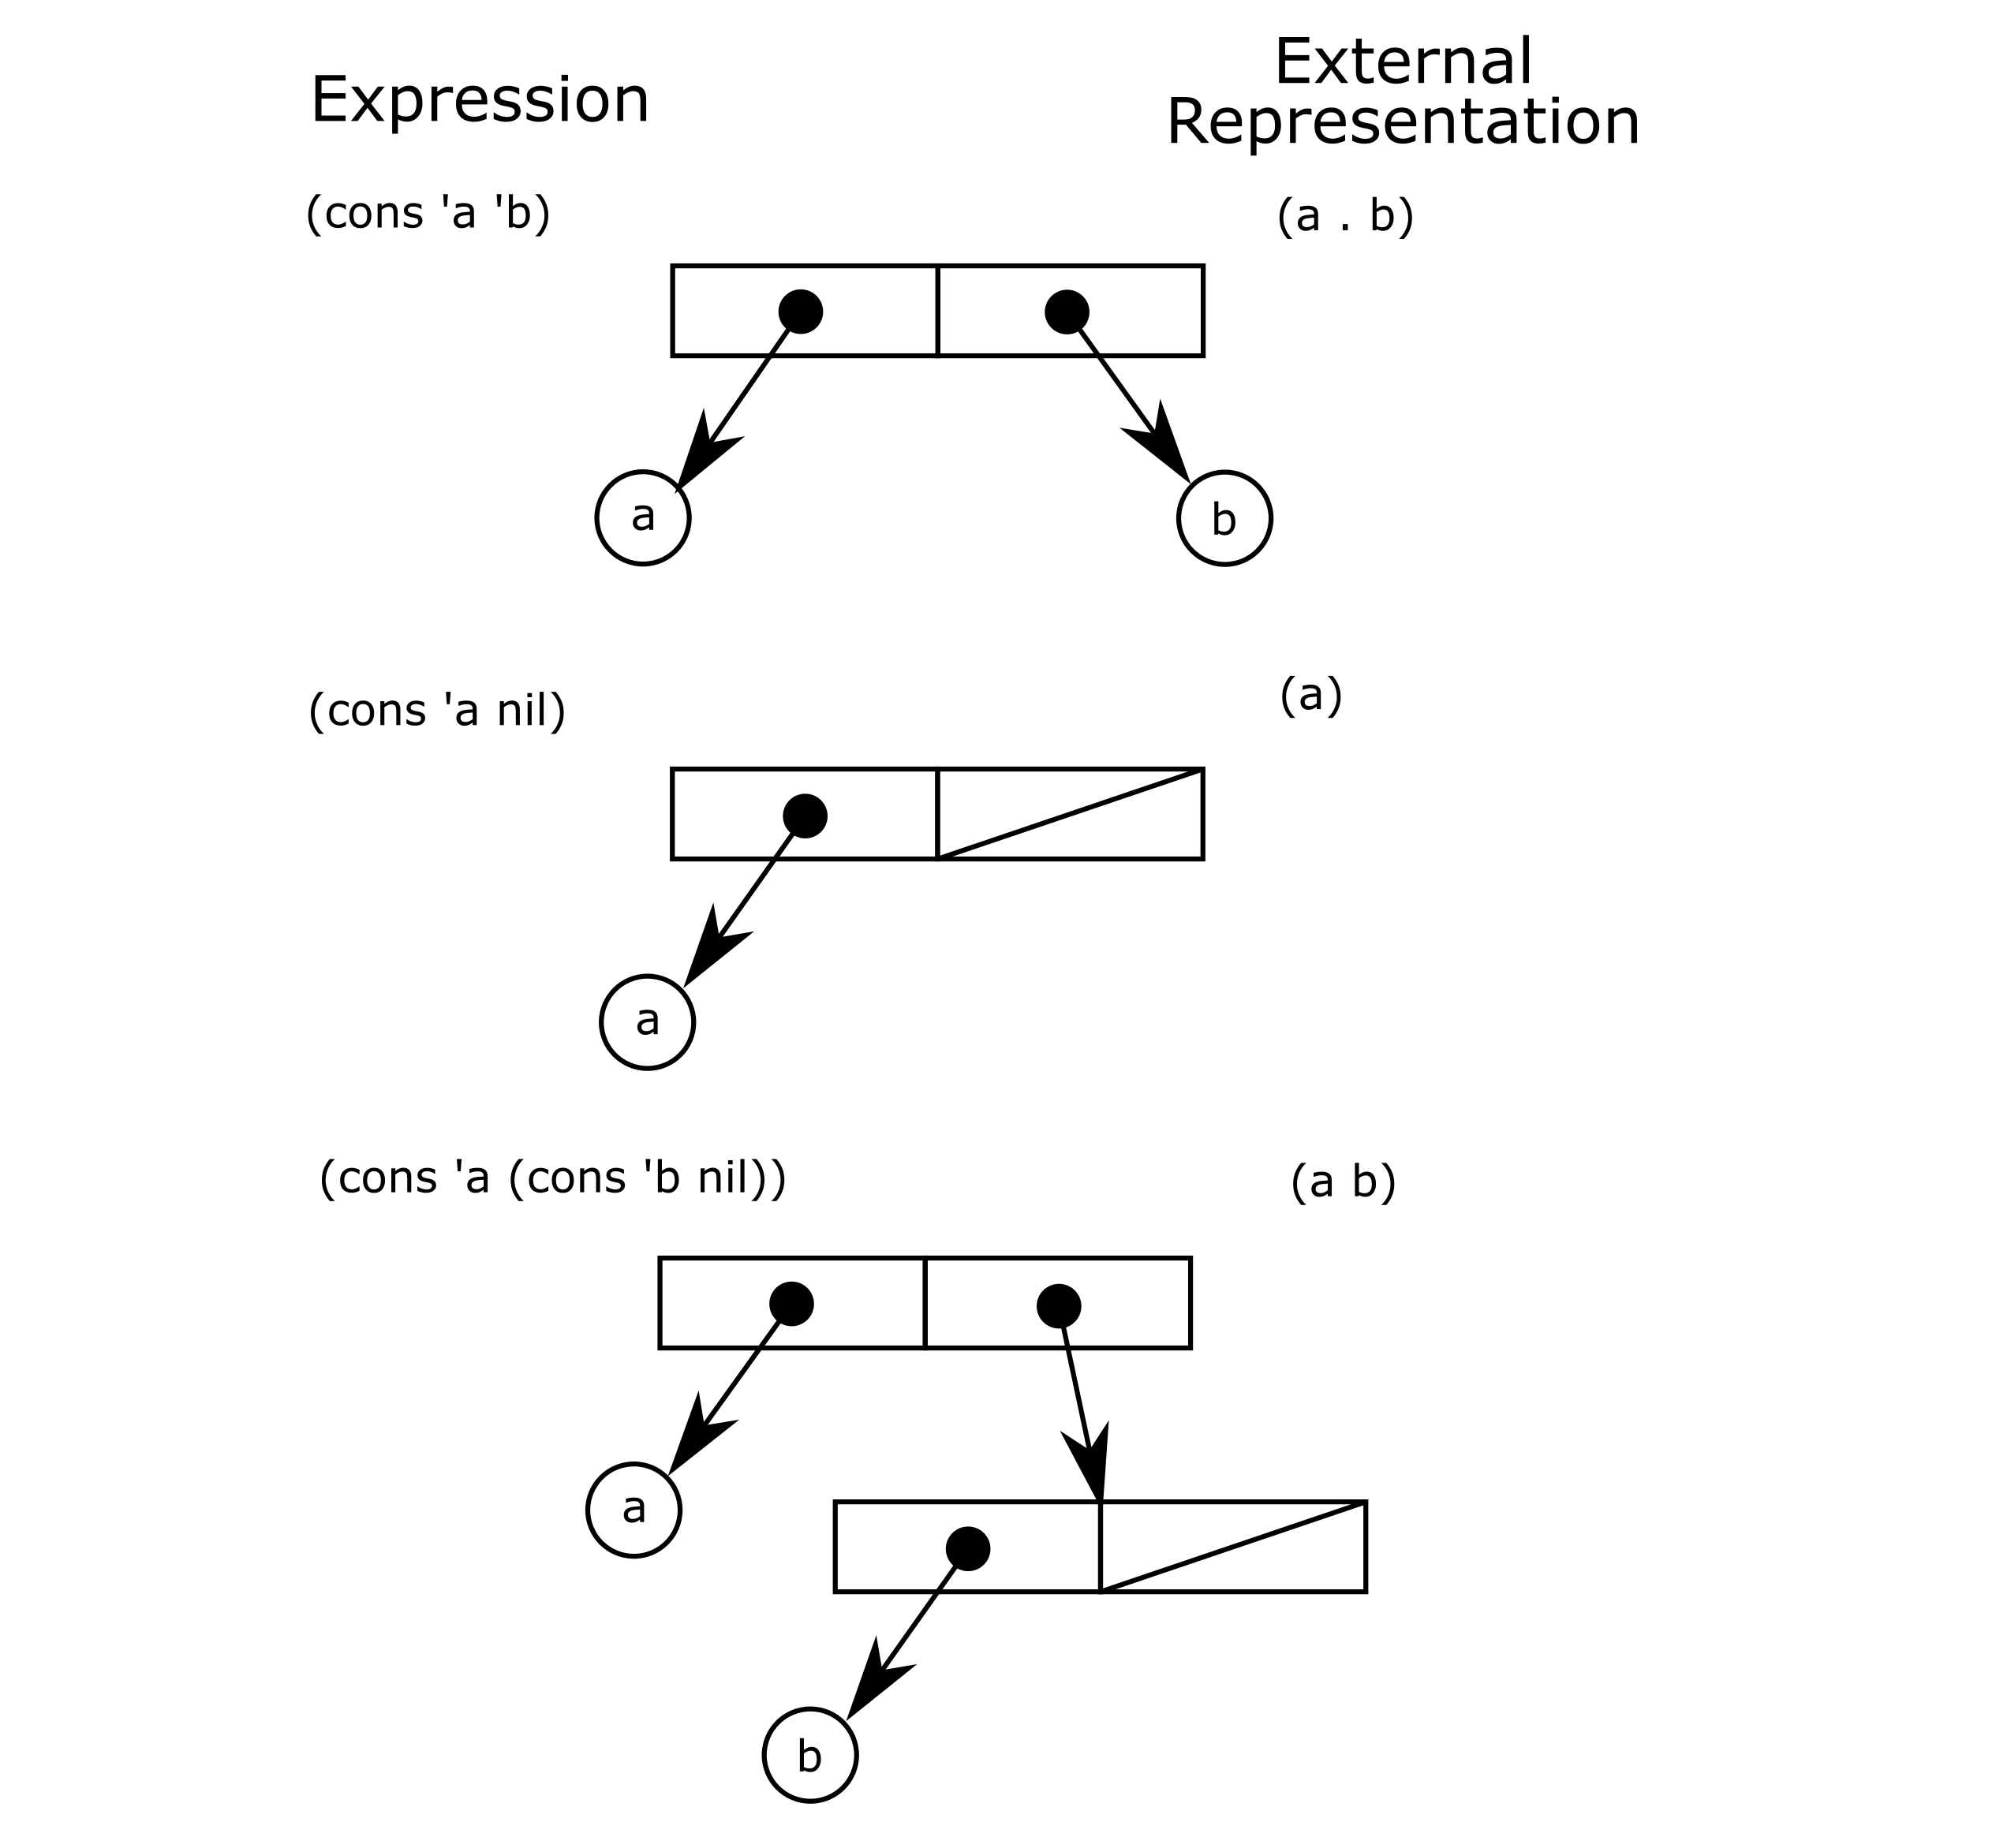
\includegraphics{images/consing.png}
\noindent\begin{tabular}{ |p{1.5cm} p{8cm}| }
\hline
\rowcolor[HTML]{CCCCCC} \multicolumn{2}{|l|}{\bf cons (public)} \\
car & a Lisp value \\
cdr & a Lisp value \\
\textit{Returns:} & a pair \\
\hline
\end{tabular}
\index{cons}
\begin{lstlisting}
reg cons
 
proc ::constcl::cons {car cdr} {
  MkPair $car $cdr
}
\end{lstlisting}


\textbf{car} procedure


\texttt{car} gets the contents of the first cell in a pair.



Example:

\begin{verbatim}
(car '(a b))   =>  a
\end{verbatim}
\noindent\begin{tabular}{ |p{1.5cm} p{8cm}| }
\hline
\rowcolor[HTML]{CCCCCC} \multicolumn{2}{|l|}{\bf car (public)} \\
pair & a pair \\
\textit{Returns:} & a Lisp value \\
\hline
\end{tabular}
\index{car}
\begin{lstlisting}
reg car
 
proc ::constcl::car {pair} {
  $pair car
}
\end{lstlisting}


\textbf{cdr} procedure


\texttt{cdr} gets the contents of the second cell in a pair.



Example:

\begin{verbatim}
(cdr '(a b))   =>  (b)
\end{verbatim}
\noindent\begin{tabular}{ |p{1.5cm} p{8cm}| }
\hline
\rowcolor[HTML]{CCCCCC} \multicolumn{2}{|l|}{\bf cdr (public)} \\
pair & a pair \\
\textit{Returns:} & a Lisp value \\
\hline
\end{tabular}
\index{cdr}
\begin{lstlisting}
reg cdr
 
proc ::constcl::cdr {pair} {
  $pair cdr
}
\end{lstlisting}


\textbf{caar} to \textbf{cddddr}


\texttt{car} and \texttt{cdr} can be combined to form 28 composite access operations.

\index{caar}
\begin{lstlisting}
foreach ads {
  aa
  ad
  da
  dd
  aaa
  ada
  daa
  dda
  aad
  add
  dad
  ddd
  aaaa
  adaa
  daaa
  ddaa
  aada
  adda
  dada
  ddda
  aaad
  adad
  daad
  ddad
  aadd
  addd
  dadd
  dddd
} {
    reg c${ads}r
 
    proc ::constcl::c${ads}r {pair} "
        foreach c \[lreverse \[split $ads {}\]\] {
            if {\$c eq \"a\"} {
                set pair \[car \$pair\]
            } else {
                set pair \[cdr \$pair\]
            }
        }
        return \$pair
    "
 
}
\end{lstlisting}


\textbf{set-car!} procedure


\texttt{set-car!} sets the contents of the first cell in a pair.



Example:

\begin{verbatim}
(let ((pair (cons 'a 'b)) (val 'x))
  (set-car! pair val))                =>  (x . b)
\end{verbatim}
\noindent\begin{tabular}{ |p{1.5cm} p{8cm}| }
\hline
\rowcolor[HTML]{CCCCCC} \multicolumn{2}{|l|}{\bf set-car! (public)} \\
pair & a pair \\
val & a Lisp value \\
\textit{Returns:} & a pair \\
\hline
\end{tabular}
\index{set-car!}
\begin{lstlisting}
reg set-car!
 
proc ::constcl::set-car! {pair val} {
  $pair set-car! $val
}
\end{lstlisting}


\textbf{set-cdr!} procedure


\texttt{set-cdr!} sets the contents of the second cell in a pair.



Example:

\begin{verbatim}
(let ((pair (cons 'a 'b)) (val 'x))
  (set-cdr! pair val))                =>  (a . x)
\end{verbatim}
\noindent\begin{tabular}{ |p{1.5cm} p{8cm}| }
\hline
\rowcolor[HTML]{CCCCCC} \multicolumn{2}{|l|}{\bf set-cdr! (public)} \\
pair & a pair \\
val & a Lisp value \\
\textit{Returns:} & a pair \\
\hline
\end{tabular}
\index{set-cdr!}
\begin{lstlisting}
reg set-cdr!
 
proc ::constcl::set-cdr! {pair val} {
  $pair set-cdr! $val
}
\end{lstlisting}


\textbf{list?} procedure


The \texttt{list?} predicate tests if a pair is part of a proper list, one that ends with NIL.

\noindent\begin{tabular}{ |p{1.5cm} p{8cm}| }
\hline
\rowcolor[HTML]{CCCCCC} \multicolumn{2}{|l|}{\bf list? (public)} \\
val & a Lisp value \\
\textit{Returns:} & a boolean \\
\hline
\end{tabular}
\index{list?}
\begin{lstlisting}
reg list?
 
proc ::constcl::list? {val} {
  set visited {}
  if {[null? $val] ne "#f"} {
      return #t
  } elseif {[pair? $val] ne "#f"} {
      return [listp $val]
  } else {
      return #f
  }
}
\end{lstlisting}


\textbf{listp} procedure


\texttt{listp} is a helper procedure that recursively traverses a cons trail to find out if it is cyclic or ends in an atom, which means that the procedure returns false, or if it ends in \texttt{\#NIL}, which means that it returns true.

\noindent\begin{tabular}{ |p{1.5cm} p{8cm}| }
\hline
\rowcolor[HTML]{CCCCCC} \multicolumn{2}{|l|}{\bf listp (internal)} \\
pair & a pair \\
\textit{Returns:} & a boolean \\
\hline
\end{tabular}
\index{listp}
\begin{lstlisting}
proc ::constcl::listp {pair} {
  upvar visited visited
  if {$pair in $visited} {
    return #f
  }
  lappend visited $pair
  if {[null? $pair] ne "#f"} {
    return #t
  } elseif {[pair? $pair] ne "#f"} {
    return [listp [cdr $pair]]
  } else {
    return #f
  }
}
\end{lstlisting}


\textbf{list} procedure


\texttt{list} constructs a Lisp list from a number of values.



Example:

\begin{verbatim}
(list 1 2 3)   =>  (1 2 3)
\end{verbatim}
\noindent\begin{tabular}{ |p{1.5cm} p{8cm}| }
\hline
\rowcolor[HTML]{CCCCCC} \multicolumn{2}{|l|}{\bf list (public)} \\
args & some Lisp values \\
\textit{Returns:} & a Lisp list of Lisp values \\
\hline
\end{tabular}
\index{list}
\begin{lstlisting}
reg list
 
proc ::constcl::list {args} {
  if {[llength $args] == 0} {
    return #NIL
  } else {
    set prev #NIL
    foreach obj [lreverse $args] {
      set prev [cons $obj $prev]
    }
    return $prev
  }
}
\end{lstlisting}


\textbf{length} procedure


\texttt{length} reports the length of a Lisp list.



Example:

\begin{verbatim}
(length '(a b c d))   =>  4
\end{verbatim}
\noindent\begin{tabular}{ |p{1.5cm} p{8cm}| }
\hline
\rowcolor[HTML]{CCCCCC} \multicolumn{2}{|l|}{\bf length (public)} \\
pair & a pair \\
\textit{Returns:} & a number \\
\hline
\end{tabular}
\index{length}
\begin{lstlisting}
reg length
 
proc ::constcl::length {pair} {
  check {list? $pair} {
    LIST expected\n([pn] lst)
  }
  MkNumber [length-helper $pair]
}
\end{lstlisting}


\textbf{length-helper} procedure


\texttt{length-helper} is a helper procedure which measures a list recursively.

\noindent\begin{tabular}{ |p{1.5cm} p{8cm}| }
\hline
\rowcolor[HTML]{CCCCCC} \multicolumn{2}{|l|}{\bf length-helper (internal)} \\
pair & a pair \\
\textit{Returns:} & a Tcl number \\
\hline
\end{tabular}
\index{length-helper}
\begin{lstlisting}
proc ::constcl::length-helper {pair} {
  if {[null? $pair] ne "#f"} {
    return 0
  } else {
    return [expr {1 +
      [length-helper [cdr $pair]]}]
  }
}
\end{lstlisting}


\textbf{append} procedure


\texttt{append} joins lists together.



Example:

\begin{verbatim}
(append '(a b) '(c d))   =>  (a b c d)
\end{verbatim}
\noindent\begin{tabular}{ |p{1.5cm} p{8cm}| }
\hline
\rowcolor[HTML]{CCCCCC} \multicolumn{2}{|l|}{\bf append (public)} \\
args & some lists \\
\textit{Returns:} & a Lisp list of Lisp values \\
\hline
\end{tabular}
\index{append}
\begin{lstlisting}
reg append
 
proc ::constcl::append {args} {
  set prev [lindex $args end]
  foreach r [lreverse [lrange $args 0 end-1]] {
    check {list? $r} {
      LIST expected\n([pn] [$r show])
    }
    set prev [copy-list $r $prev]
  }
  set prev
}
\end{lstlisting}


\textbf{copy-list} procedure


\texttt{copy-list} joins together two lists by recursively consing items from the first list towards the second.

\noindent\begin{tabular}{ |p{1.5cm} p{8cm}| }
\hline
\rowcolor[HTML]{CCCCCC} \multicolumn{2}{|l|}{\bf copy-list (internal)} \\
pair & a pair \\
next & a Lisp list of Lisp values \\
\textit{Returns:} & a Lisp list of Lisp values \\
\hline
\end{tabular}
\index{copy-list}
\begin{lstlisting}
proc ::constcl::copy-list {pair next} {
  # TODO only fresh conses in the direct chain to NIL
  if {[null? $pair] ne "#f"} {
    set next
  } elseif {[null? [cdr $pair]] ne "#f"} {
    cons [car $pair] $next
  } else {
    cons [car $pair] [copy-list [cdr $pair] $next]
  }
}
\end{lstlisting}


\textbf{reverse} procedure


\texttt{reverse} produces a reversed copy of a Lisp list.



Example:

\begin{verbatim}
(reverse '(a b c))   =>  (c b a)
\end{verbatim}
\noindent\begin{tabular}{ |p{1.5cm} p{8cm}| }
\hline
\rowcolor[HTML]{CCCCCC} \multicolumn{2}{|l|}{\bf reverse (public)} \\
vals & a Lisp list of Lisp values \\
\textit{Returns:} & a Lisp list of Lisp values \\
\hline
\end{tabular}
\index{reverse}
\begin{lstlisting}
reg reverse
 
proc ::constcl::reverse {vals} {
  list {*}[lreverse [splitlist $vals]]
}
\end{lstlisting}


\textbf{list-tail} procedure


Given a list index, \texttt{list-tail} yields the sublist starting from that index.



Example:

\begin{verbatim}
(let ((lst '(a b c d e f)) (k 3))
  (list-tail lst k))                =>  (d e f)
\end{verbatim}
\noindent\begin{tabular}{ |p{1.5cm} p{8cm}| }
\hline
\rowcolor[HTML]{CCCCCC} \multicolumn{2}{|l|}{\bf list-tail (public)} \\
vals & a Lisp list of Lisp values \\
k & a number \\
\textit{Returns:} & a Lisp list of Lisp values \\
\hline
\end{tabular}
\index{list-tail}
\begin{lstlisting}
reg list-tail
 
proc ::constcl::list-tail {vals k} {
  if {[zero? $k] ne "#f"} {
    return $vals
  } else {
    list-tail [cdr $vals] [- $k #1]
  }
}
\end{lstlisting}


\textbf{list-ref} procedure


\texttt{list-ref} yields the list item at a given index.



Example:

\begin{verbatim}
(let ((lst '(a b c d e f)) (k 3))
  (list-ref lst k))                 =>  d
\end{verbatim}
\noindent\begin{tabular}{ |p{1.5cm} p{8cm}| }
\hline
\rowcolor[HTML]{CCCCCC} \multicolumn{2}{|l|}{\bf list-ref (public)} \\
vals & a Lisp list of Lisp values \\
k & a number \\
\textit{Returns:} & a Lisp value \\
\hline
\end{tabular}
\index{list-ref}
\begin{lstlisting}
reg list-ref
 
proc ::constcl::list-ref {vals k} {
  car [list-tail $vals $k]
}
\end{lstlisting}


\textbf{memq} procedure


\textbf{memv} procedure


\textbf{member} procedure


\texttt{memq}, \texttt{memv}, and \texttt{member} return the sublist starting with a given item, or \texttt{\#f} if there is none. They use \texttt{eq?}, \texttt{eqv?}, and \texttt{equal?}, respectively, for the comparison.



Example:

\begin{verbatim}
(let ((lst '(a b c d e f)) (val 'd))
  (memq val lst))                      =>  (d e f)
\end{verbatim}
\noindent\begin{tabular}{ |p{1.5cm} p{8cm}| }
\hline
\rowcolor[HTML]{CCCCCC} \multicolumn{2}{|l|}{\bf memq (public)} \\
val1 & a Lisp value \\
val2 & a Lisp list of Lisp values \\
\textit{Returns:} & a Lisp list of values OR \#f \\
\hline
\end{tabular}
\index{memq}
\begin{lstlisting}
reg memq
 
proc ::constcl::memq {val1 val2} {
  return [member-proc eq? $val1 $val2]
}
\end{lstlisting}
\noindent\begin{tabular}{ |p{1.5cm} p{8cm}| }
\hline
\rowcolor[HTML]{CCCCCC} \multicolumn{2}{|l|}{\bf memv (public)} \\
val1 & a Lisp value \\
val2 & a Lisp list of Lisp values \\
\textit{Returns:} & a Lisp list of values OR \#f \\
\hline
\end{tabular}
\index{memv}
\begin{lstlisting}
reg memv
 
proc ::constcl::memv {val1 val2} {
  return [member-proc eqv? $val1 $val2]
}
\end{lstlisting}
\noindent\begin{tabular}{ |p{1.5cm} p{8cm}| }
\hline
\rowcolor[HTML]{CCCCCC} \multicolumn{2}{|l|}{\bf member (public)} \\
val1 & a Lisp value \\
val2 & a Lisp list of Lisp values \\
\textit{Returns:} & a Lisp list of values OR \#f \\
\hline
\end{tabular}
\index{member}
\begin{lstlisting}
reg member
 
proc ::constcl::member {val1 val2} {
  return [member-proc equal? $val1 $val2]
}
\end{lstlisting}


\textbf{member-proc} procedure


\texttt{member-proc} helper procedure which does the work for the \texttt{memq}, \texttt{memv}, and \texttt{member} procedures. Works by recursively taking the \texttt{cdr} of the list, comparing against the \texttt{car} of the list.

\noindent\begin{tabular}{ |p{1.5cm} p{8cm}| }
\hline
\rowcolor[HTML]{CCCCCC} \multicolumn{2}{|l|}{\bf member-proc (internal)} \\
epred & an equivalence predicate \\
val1 & a Lisp value \\
val2 & a Lisp list of Lisp values \\
\textit{Returns:} & a Lisp list of values OR \#f \\
\hline
\end{tabular}
\index{member-proc}
\begin{lstlisting}
proc ::constcl::member-proc {epred val1 val2} {
  switch $epred {
    eq? { set name "memq" }
    eqv? { set name "memv" }
    equal? { set name "member" }
  }
  check {list? $val2} {
    LIST expected\n($name [$val1 show] [$val2 show])
  }
  if {[null? $val2] ne "#f"} {
    return #f
  } elseif {[pair? $val2] ne "#f"} {
    if {[$epred $val1 [car $val2]] ne "#f"} {
      return $val2
    } else {
      return [member-proc $epred $val1 [cdr $val2]]
    }
  }
}
\end{lstlisting}


\textbf{assq} procedure


\textbf{assv} procedure


\textbf{assoc} procedure


\texttt{assq}, \texttt{assv}, and \texttt{assoc} return the associative item marked with a given key, or \texttt{\#f} if there is none. They use \texttt{eq?}, \texttt{eqv?}, and \texttt{equal?}, respectively, for the comparison. They implement lookup in the form of lookup table known as an association list, or \emph{alist}.


Example:

\begin{verbatim}
(define e '((a 1) (b 2) (c 3)))
(assq 'a e)                       => (a 1)
\end{verbatim}
\noindent\begin{tabular}{ |p{1.5cm} p{8cm}| }
\hline
\rowcolor[HTML]{CCCCCC} \multicolumn{2}{|l|}{\bf assq (public)} \\
val1 & a Lisp value \\
val2 & an association list \\
\textit{Returns:} & a Lisp list of values OR \#f \\
\hline
\end{tabular}
\index{assq}
\begin{lstlisting}
reg assq
 
proc ::constcl::assq {val1 val2} {
  return [assoc-proc eq? $val1 $val2]
}
\end{lstlisting}
\noindent\begin{tabular}{ |p{1.5cm} p{8cm}| }
\hline
\rowcolor[HTML]{CCCCCC} \multicolumn{2}{|l|}{\bf assv (public)} \\
val1 & a Lisp value \\
val2 & an association list \\
\textit{Returns:} & a Lisp list of values OR \#f \\
\hline
\end{tabular}
\index{assv}
\begin{lstlisting}
reg assv
 
proc ::constcl::assv {val1 val2} {
  return [assoc-proc eqv? $val1 $val2]
}
\end{lstlisting}
\noindent\begin{tabular}{ |p{1.5cm} p{8cm}| }
\hline
\rowcolor[HTML]{CCCCCC} \multicolumn{2}{|l|}{\bf assoc (public)} \\
val1 & a Lisp value \\
val2 & an association list \\
\textit{Returns:} & a Lisp list of values OR \#f \\
\hline
\end{tabular}
\index{assoc}
\begin{lstlisting}
reg assoc
 
proc ::constcl::assoc {val1 val2} {
  return [assoc-proc equal? $val1 $val2]
}
\end{lstlisting}


\textbf{assoc-proc} procedure


\texttt{assoc-proc} is a helper procedure which does the work for \texttt{assq}, \texttt{assv}, and \texttt{assoc}.

\noindent\begin{tabular}{ |p{1.5cm} p{8cm}| }
\hline
\rowcolor[HTML]{CCCCCC} \multicolumn{2}{|l|}{\bf assoc-proc (internal)} \\
epred & an equivalence predicate \\
val1 & a Lisp value \\
val2 & an association list \\
\textit{Returns:} & a Lisp list of values OR \#f \\
\hline
\end{tabular}
\index{assoc-proc}
\begin{lstlisting}
proc ::constcl::assoc-proc {epred val1 val2} {
  switch $epred {
    eq? { set name "assq" }
    eqv? { set name "assv" }
    equal? { set name "assoc" }
  }
  check {list? $val2} {
    LIST expected\n($name [$val1 show] [$val2 show])
  }
  if {[null? $val2] ne "#f"} {
    return #f
  } elseif {[pair? $val2] ne "#f"} {
    if {[pair? [car $val2]] ne "#f" && 
      [$epred $val1 [caar $val2]] ne "#f"} {
      return [car $val2]
    } else {
      return [assoc-proc $epred $val1 [cdr $val2]]
    }
  }
}
\end{lstlisting}
\section{Strings}
\label{strings}
\index{strings}


Procedures for dealing with strings of characters.


\textbf{String} class


Strings have the internal representation of a vector of character objects, with the data elements of the vector address of the first element, and the length of the vector. External representation is surrounded by double quotes, with double quotes and backslashes within the string escaped with a backslash.


As a ConsTcl extension, a \texttt{\textbackslash\ n} pair in the external representation is stored as a newline character. It is restored to \texttt{\textbackslash\ n} on write.

\index{String}
\begin{lstlisting}
oo::class create ::constcl::String {
  superclass ::constcl::NIL
  variable data constant
  constructor {v} {
    set v [::string trim $v "\""]
    set v [string map {\\\\ \\ \\\" \" \\n \n} $v]
    set len [::string length $v]
    set vsa [::constcl::vsAlloc $len]
    set idx $vsa
    foreach elt [split $v {}] {
      if {$elt eq " "} {
        set c #\\space
      } elseif {$elt eq "\n"} {
        set c #\\newline
      } else {
        set c #\\$elt
      }
      lset ::constcl::vectorSpace $idx \
        [::constcl::MkChar $c]
      incr idx
    }
    set data [
      ::constcl::cons [N $vsa] [N $len]]
    set constant 0
  }
  method = {str} {
    ::string equal [my value] [$str value]
  }
  method cmp {str} {
    ::string compare [my value] [$str value]
  }
  method length {} {
    ::constcl::cdr $data
  }
  method ref {k} {
    set k [$k numval]
    if {$k < 0 || $k >= [[my length] numval]} {
      ::error "index out of range\n$k"
    }
    lindex [my store] $k
  }
  method store {} {
    set base [[::constcl::car $data] numval]
    set end [expr {[[my length] numval] +
      $base - 1}]
    lrange $::constcl::vectorSpace $base $end
  }
  method value {} {
    join [lmap c [my store] {$c char}] {}
  }
  method set! {k c} {
    if {[my constant]} {
      ::error "string is constant"
    } else {
      set k [$k numval]
      if {$k < 0 ||
        $k >= [[my length] numval]} {
        ::error "index out of range\n$k"
      }
      set base [[::constcl::car $data] numval]
      lset ::constcl::vectorSpace $k+$base $c
    }
    return [self]
  }
  method fill! {c} {
    if {[my constant]} {
      ::error "string is constant"
    } else {
      set base [[::constcl::car $data] numval]
      set len [[my length] numval]
      for {set idx $base} \
        {$idx < $len+$base} \
        {incr idx} {
        lset ::constcl::vectorSpace $idx $c
      }
    }
    return [self]
  }
  method substring {from to} {
    join [lmap c [lrange [my store] \
      [$from numval] [$to numval]] {$c char}] {}
  }
  method mkconstant {} {
    set constant 1
  }
  method constant {} {
    set constant
  }
  method external {} {
    return "\"[
      string map {\\ \\\\ \" \\\" \n \\n} [my value]]\""
  }
  method write {handle} {
    puts -nonewline $handle [my external]
  }
  method display {handle} {
    puts -nonewline $handle [my value]
  }
  method show {} {
    my external
  }
}
\end{lstlisting}


\textbf{MkString} generator


\texttt{MkString} generates a String object.

\noindent\begin{tabular}{ |p{1.5cm} p{8cm}| }
\hline
\rowcolor[HTML]{CCCCCC} \multicolumn{2}{|l|}{\bf MkString (internal)} \\
str & an external rep of a string \\
\textit{Returns:} & a string \\
\hline
\end{tabular}
\index{MkString}
\begin{lstlisting}
interp alias {} ::constcl::MkString \
  {} ::constcl::String new
\end{lstlisting}


\textbf{string?} procedure


\texttt{string?} recognizes a string by type.

\noindent\begin{tabular}{ |p{1.5cm} p{8cm}| }
\hline
\rowcolor[HTML]{CCCCCC} \multicolumn{2}{|l|}{\bf string? (public)} \\
val & a Lisp value \\
\textit{Returns:} & a boolean \\
\hline
\end{tabular}
\index{string?}
\begin{lstlisting}
reg string?
 
proc ::constcl::string? {val} {
  typeof? $val String
}
\end{lstlisting}


\textbf{make-string} procedure


\texttt{make-string} creates a string of \emph{k} characters, optionally filled with \emph{char} characters. If \emph{char} is omitted, the string will be filled with space characters.



Example:

\begin{verbatim}
(let ((k 5))
  (make-string k))        =>  "     "
(let ((k 5) (char #\A))
  (make-string k char))   =>  "AAAAA"
\end{verbatim}
\noindent\begin{tabular}{ |p{1.5cm} p{8cm}| }
\hline
\rowcolor[HTML]{CCCCCC} \multicolumn{2}{|l|}{\bf make-string (public)} \\
k & a number \\
?char? & a character \\
\textit{Returns:} & a string \\
\hline
\end{tabular}
\index{make-string}
\begin{lstlisting}
reg make-string
 
proc ::constcl::make-string {k args} {
  set i [$k numval]
  if {[llength $args] == 0} {
    set char " "
  } else {
    lassign $args c
    set char [$c char]
  }
  return [MkString [::string repeat $char $i]]
}
\end{lstlisting}


\textbf{string} procedure


\texttt{string} constructs a string from a number of Lisp characters.



Example:

\begin{verbatim}
(string #\f #\o #\o)   =>  "foo"
\end{verbatim}
\noindent\begin{tabular}{ |p{1.5cm} p{8cm}| }
\hline
\rowcolor[HTML]{CCCCCC} \multicolumn{2}{|l|}{\bf string (public)} \\
args & some characters \\
\textit{Returns:} & a string \\
\hline
\end{tabular}
\index{string}
\begin{lstlisting}
reg string
 
proc ::constcl::string {args} {
  set str {}
  foreach char $args {
    check {::constcl::char? $char} {
      CHAR expected\n([pn] [lmap c $args \
        {$c show}])
    }
    ::append str [$char char]
  }
  return [MkString $str]
}
\end{lstlisting}


\textbf{string-length} procedure


\texttt{string-length} reports a string's length.



Example:

\begin{verbatim}
(string-length "foobar")   => 6
\end{verbatim}
\noindent\begin{tabular}{ |p{1.5cm} p{8cm}| }
\hline
\rowcolor[HTML]{CCCCCC} \multicolumn{2}{|l|}{\bf string-length (public)} \\
str & a string \\
\textit{Returns:} & a number \\
\hline
\end{tabular}
\index{string-length}
\begin{lstlisting}
reg string-length
 
proc ::constcl::string-length {str} {
  check {::constcl::string? $str} {
    STRING expected\n([pn] [$str show])
  }
  return [$str length]
}
\end{lstlisting}


\textbf{string-ref} procedure


\texttt{string-ref} yields the \emph{k}-th character (0-based) in \emph{str}.



Example:

\begin{verbatim}
(string-ref "foobar" 3)   => #\b
\end{verbatim}
\noindent\begin{tabular}{ |p{1.5cm} p{8cm}| }
\hline
\rowcolor[HTML]{CCCCCC} \multicolumn{2}{|l|}{\bf string-ref (public)} \\
str & a string \\
k & a number \\
\textit{Returns:} & a character \\
\hline
\end{tabular}
\index{string-ref}
\begin{lstlisting}
reg string-ref
 
proc ::constcl::string-ref {str k} {
  check {::constcl::string? $str} {
    STRING expected\n([pn] [$str show] \
      [$k show])
  }
  check {::constcl::number? $k} {
    INTEGER expected\n([pn] [$str show] \
      [$k show])
  }
  return [$str ref $k]
}
\end{lstlisting}


\textbf{string-set!} procedure


\texttt{string-set!} replaces the character at \emph{k} with \emph{char} in a non-constant string.



Example:

\begin{verbatim}
(let ((str (string #\f #\o #\o))
      (k 2)
      (char #\x))
  (string-set! str k char))         =>  "fox"
\end{verbatim}
\noindent\begin{tabular}{ |p{1.5cm} p{8cm}| }
\hline
\rowcolor[HTML]{CCCCCC} \multicolumn{2}{|l|}{\bf string-set! (public)} \\
str & a string \\
k & a number \\
char & a character \\
\textit{Returns:} & a string \\
\hline
\end{tabular}
\index{string-set!}
\begin{lstlisting}
reg string-set!
 
proc ::constcl::string-set! {str k char} {
  check {string? $str} {
    STRING expected\n([pn] [$str show] [$k show] \
      [$char show])
  }
  check {number? $k} {
    INTEGER expected\n([pn] [$str show] \
      [$k show] [$char show])
  }
  check {char? $char} {
    CHAR expected\n([pn] [$str show] [$k show] \
      [$char show])
  }
  $str set! $k $char
  return $str
}
\end{lstlisting}


\textbf{string=?}, \textbf{string-ci=?}


\textbf{string<?}, \textbf{string-ci<?}


\textbf{string>?}, \textbf{string-ci>?}


\textbf{string<=?}, \textbf{string-ci<=?}


\textbf{string>=?}, \textbf{string-ci>=?}


\texttt{string=?}, \texttt{string<?}, \texttt{string>?}, \texttt{string<=?}, \texttt{string>=?} and their case insensitive variants \texttt{string-ci=?}, \texttt{string-ci<?}, \texttt{string-ci>?}, \texttt{string-ci<=?}, \texttt{string-ci>=?} compare strings.

\noindent\begin{tabular}{ |p{1.5cm} p{8cm}| }
\hline
\rowcolor[HTML]{CCCCCC} \multicolumn{2}{|l|}{\bf string=?, string<?, string>? (public)} \\
str1 & a string \\
str2 & a string \\
\textit{Returns:} & a boolean \\
\hline
\end{tabular}
\noindent\begin{tabular}{ |p{1.5cm} p{8cm}| }
\hline
\rowcolor[HTML]{CCCCCC} \multicolumn{2}{|l|}{\bf string<=?, string>=? (public)} \\
str1 & a string \\
str2 & a string \\
\textit{Returns:} & a boolean \\
\hline
\end{tabular}
\noindent\begin{tabular}{ |p{1.5cm} p{8cm}| }
\hline
\rowcolor[HTML]{CCCCCC} \multicolumn{2}{|l|}{\bf string-ci=?, string-ci<?, string-ci>? (public)} \\
str1 & a string \\
str2 & a string \\
\textit{Returns:} & a boolean \\
\hline
\end{tabular}
\noindent\begin{tabular}{ |p{1.5cm} p{8cm}| }
\hline
\rowcolor[HTML]{CCCCCC} \multicolumn{2}{|l|}{\bf string-ci<=?, string-ci>=? (public)} \\
str1 & a string \\
str2 & a string \\
\textit{Returns:} & a boolean \\
\hline
\end{tabular}
\index{string=!}
\begin{lstlisting}
reg string=?
 
proc ::constcl::string=? {str1 str2} {
  check {string? $str1} {
    STRING expected\n([pn] [$str1 show] \
      [$str2 show])
  }
  check {string? $str2} {
    STRING expected\n([pn] [$str1 show] \
      [$str2 show])
  }
  if {[$str1 value] eq [$str2 value]} {
    return #t
  } else {
    return #f
  }
}
\end{lstlisting}
\index{string-ci=!}
\begin{lstlisting}
reg string-ci=?
 
proc ::constcl::string-ci=? {str1 str2} {
  check {string? $str1} {
    STRING expected\n([pn] [$str1 show] \
      [$str2 show])
  }
  check {string? $str2} {
    STRING expected\n([pn] [$str1 show] \
      [$str2 show])
  }
  if {[::string tolower [$str1 value]] eq
      [::string tolower [$str2 value]]} {
    return #t
  } else {
    return #f
  }
}
\end{lstlisting}
\index{string<!}
\begin{lstlisting}
reg string<?
 
proc ::constcl::string<? {str1 str2} {
  check {string? $str1} {
    STRING expected\n([pn] [$str1 show] \
      [$str2 show])
  }
  check {string? $str2} {
    STRING expected\n([pn] [$str1 show] \
      [$str2 show])
  }
  if {[$str1 value] < [$str2 value]} {
    return #t
  } else {
    return #f
  }
}
\end{lstlisting}
\index{string-ci<!}
\begin{lstlisting}
reg string-ci<?
 
proc ::constcl::string-ci<? {str1 str2} {
  check {string? $str1} {
    STRING expected\n([pn] [$str1 show] \
      [$str2 show])
  }
  check {string? $str2} {
    STRING expected\n([pn] [$str1 show] \
      [$str2 show])
  }
  if {[::string tolower [$str1 value]] <
      [::string tolower [$str2 value]]} {
    return #t
  } else {
    return #f
  }
}
\end{lstlisting}
\index{string>!}
\begin{lstlisting}
reg string>?
 
proc ::constcl::string>? {str1 str2} {
  check {string? $str1} {
    STRING expected\n([pn] [$str1 show] \
      [$str2 show])
  }
  check {string? $str2} {
    STRING expected\n([pn] [$str1 show] \
      [$str2 show])
  }
  if {[$str1 value] > [$str2 value]} {
    return #t
  } else {
    return #f
  }
}
\end{lstlisting}
\index{string-ci>!}
\begin{lstlisting}
reg string-ci>?
 
proc ::constcl::string-ci>? {str1 str2} {
  check {string? $str1} {
    STRING expected\n([pn] [$str1 show] \
      [$str2 show])
  }
  check {string? $str2} {
    STRING expected\n([pn] [$str1 show] \
      [$str2 show])
  }
  if {[::string tolower [$str1 value]] >
      [::string tolower [$str2 value]]} {
    return #t
  } else {
    return #f
  }
}
\end{lstlisting}
\index{string<=!}
\begin{lstlisting}
reg string<=?
 
proc ::constcl::string<=? {str1 str2} {
  check {string? $str1} {
    STRING expected\n([pn] [$str1 show] \
      [$str2 show])
  }
  check {string? $str2} {
    STRING expected\n([pn] [$str1 show] \
      [$str2 show])
  }
  if {[$str1 value] <= [$str2 value]} {
    return #t
  } else {
    return #f
  }
}
\end{lstlisting}
\index{string-ci<=!}
\begin{lstlisting}
reg string-ci<=?
 
proc ::constcl::string-ci<=? {str1 str2} {
  check {string? $str1} {
    STRING expected\n([pn] [$str1 show] \
      [$str2 show])
  }
  check {string? $str2} {
    STRING expected\n([pn] [$str1 show] \
      [$str2 show])
  }
  if {[::string tolower [$str1 value]] <=
      [::string tolower [$str2 value]]} {
    return #t
  } else {
    return #f
  }
}
\end{lstlisting}
\index{string>=!}
\begin{lstlisting}
reg string>=?
 
proc ::constcl::string>=? {str1 str2} {
  check {string? $str1} {
    STRING expected\n([pn] [$str1 show] \
      [$str2 show])
  }
  check {string? $str2} {
    STRING expected\n([pn] [$str1 show] \
      [$str2 show])
  }
  if {[$str1 value] >= [$str2 value]} {
    return #t
  } else {
    return #f
  }
}
\end{lstlisting}
\index{string-ci>=!}
\begin{lstlisting}
reg string-ci>=?
 
proc ::constcl::string-ci>=? {str1 str2} {
  check {string? $str1} {
    STRING expected\n([pn] [$str1 show] \
      [$str2 show])
  }
  check {string? $str2} {
    STRING expected\n([pn] [$str1 show] \
      [$str2 show])
  }
  if {[::string tolower [$str1 value]] >=
      [::string tolower [$str2 value]]} {
    return #t
  } else {
    return #f
  }
}
\end{lstlisting}


\textbf{substring} procedure


\texttt{substring} yields the substring of \emph{str} that starts at \emph{start} and ends at \emph{end}.



Example:

\begin{verbatim}
(substring "foobar" 2 4)   => "oba"
\end{verbatim}
\noindent\begin{tabular}{ |p{1.5cm} p{8cm}| }
\hline
\rowcolor[HTML]{CCCCCC} \multicolumn{2}{|l|}{\bf substring (public)} \\
str & a string \\
start & a number \\
end & a number \\
\textit{Returns:} & a string \\
\hline
\end{tabular}
\index{substring}
\begin{lstlisting}
reg substring
 
proc ::constcl::substring {str start end} {
  check {string? $str} {
    STRING expected\n([pn] [$str show] \
      [$start show] [$end show])
  }
  check {number? $start} {
    NUMBER expected\n([pn] [$str show] \
      [$start show] [$end show])
  }
  check {number? $end} {
    NUMBER expected\n([pn] [$str show] \
      [$start show] [$end show])
  }
  return [MkString [$str substring $start $end]]
}
\end{lstlisting}


\textbf{string-append} procedure


\texttt{string-append} joins strings together.



Example:

\begin{verbatim}
(string-append "foo" "bar")   =>  "foobar"
\end{verbatim}
\noindent\begin{tabular}{ |p{1.5cm} p{8cm}| }
\hline
\rowcolor[HTML]{CCCCCC} \multicolumn{2}{|l|}{\bf string-append (public)} \\
args & some strings \\
\textit{Returns:} & a string \\
\hline
\end{tabular}
\index{string-append}
\begin{lstlisting}
reg string-append
 
proc ::constcl::string-append {args} {
    MkString [::append --> {*}[lmap arg $args {
      $arg value
    }]]
}
\end{lstlisting}


\textbf{string->list} procedure


\texttt{string->list} converts a string to a Lisp list of characters.



Example:

\begin{verbatim}
(string->list "foo")   =>  (#\f #\o #\o)
\end{verbatim}
\noindent\begin{tabular}{ |p{1.5cm} p{8cm}| }
\hline
\rowcolor[HTML]{CCCCCC} \multicolumn{2}{|l|}{\bf string->list (public)} \\
str & a string \\
\textit{Returns:} & a Lisp list of characters \\
\hline
\end{tabular}
\index{string->list}
\begin{lstlisting}
reg string->list
 
proc ::constcl::string->list {str} {
  list {*}[$str store]
}
\end{lstlisting}


\textbf{list->string} procedure


\texttt{list->string} converts a Lisp list of characters to a string.



Example:

\begin{verbatim}
(list->string '(#\1 #\2 #\3))   => "123"
\end{verbatim}
\noindent\begin{tabular}{ |p{1.5cm} p{8cm}| }
\hline
\rowcolor[HTML]{CCCCCC} \multicolumn{2}{|l|}{\bf list->string (public)} \\
list & a Lisp list of characters \\
\textit{Returns:} & a string \\
\hline
\end{tabular}
\index{list->string}
\begin{lstlisting}
reg list->string
 
proc ::constcl::list->string {list} {
  MkString [::append --> {*}[
    lmap c [splitlist $list] {$c char}]]
}
\end{lstlisting}


\textbf{string-copy} procedure


\texttt{string-copy} makes a copy of a string.



Example:

\begin{verbatim}
(let ((str (string-copy "abc"))
      (k 0)
      (char #\x))
  (string-set! str k char))       =>  "xbc"
\end{verbatim}
\noindent\begin{tabular}{ |p{1.5cm} p{8cm}| }
\hline
\rowcolor[HTML]{CCCCCC} \multicolumn{2}{|l|}{\bf string-copy (public)} \\
str & a string \\
\textit{Returns:} & a string \\
\hline
\end{tabular}
\index{string-copy}
\begin{lstlisting}
reg string-copy
 
proc ::constcl::string-copy {str} {
  check {string? $str} {
    STRING expected\n([pn] [$str show])
  }
  return [MkString [$str value]]
}
\end{lstlisting}


\textbf{string-fill!} procedure


\texttt{string-fill!} \emph{str} \emph{char} fills a non-constant string with \emph{char}.



Example:

\begin{verbatim}
(let ((str (string-copy "foobar"))
      (char #\X))
  (string-fill! str char))           =>  "XXXXXX"
\end{verbatim}
\noindent\begin{tabular}{ |p{1.5cm} p{8cm}| }
\hline
\rowcolor[HTML]{CCCCCC} \multicolumn{2}{|l|}{\bf string-fill! (public)} \\
str & a string \\
char & a character \\
\textit{Returns:} & a string \\
\hline
\end{tabular}
\index{string-fill!}
\begin{lstlisting}
reg string-fill!
 
proc ::constcl::string-fill! {str char} {
  check {string? $str} {
    STRING expected\n([pn] [$str show] \
      [$char show])
  }
  $str fill! $char
  return $str
}
\end{lstlisting}
\section{Symbols}
\label{symbols}
\index{symbols}


Symbols are like little strings that are used to refer to things (variables, including procedure names, etc) or for comparing against each other.


\textbf{Symbol} class

\index{Symbol}
\begin{lstlisting}
oo::class create ::constcl::Symbol {
  superclass ::constcl::NIL
  variable name caseconstant
  constructor {n} {
    ::constcl::idcheck $n
    set name $n
    set caseconstant 0
  }
  method name {} {
    set name
  }
  method value {} {
    set name
  }
  method = {symname} {
    if {$name eq $symname} {
      return #t
    } else {
      return #f
    }
  }
  method mkconstant {} {}
  method constant {} {
    return 1
  }
  method make-case-constant {} {
    set caseconstant 1
  }
  method case-constant {} {
    set caseconstant
  }
  method write {handle} {
    puts -nonewline $handle [my name]
  }
  method display {handle} {
    my write $handle
  }
  method show {} {
    set name
  }
}
 
unset -nocomplain ::constcl::symbolTable
set ::constcl::symbolTable [dict create]
\end{lstlisting}


\textbf{MkSymbol} generator


\texttt{MkSymbol} generates a symbol with a given name. If a symbol with that name already exists, it is returned. Otherwise, a fresh symbol is created. Short form: \texttt{S}.

\noindent\begin{tabular}{ |p{1.5cm} p{8cm}| }
\hline
\rowcolor[HTML]{CCCCCC} \multicolumn{2}{|l|}{\bf MkSymbol (internal)} \\
str & a Tcl string \\
\textit{Returns:} & a symbol \\
\hline
\end{tabular}
\index{MkSymbol}
\begin{lstlisting}
proc ::constcl::MkSymbol {str} {
  if {[dict exists $::constcl::symbolTable $str]} {
    return [dict get $::constcl::symbolTable $str]
  } else {
    set sym [::constcl::Symbol new $str]
    dict set ::constcl::symbolTable $str $sym
    return $sym
  }
}
interp alias {} S {} ::constcl::MkSymbol
\end{lstlisting}


\textbf{symbol?} procedure


\texttt{symbol?} recognizes a symbol by type.

\noindent\begin{tabular}{ |p{1.5cm} p{8cm}| }
\hline
\rowcolor[HTML]{CCCCCC} \multicolumn{2}{|l|}{\bf symbol? (public)} \\
val & a Lisp value \\
\textit{Returns:} & a boolean \\
\hline
\end{tabular}
\index{symbol?}
\begin{lstlisting}
reg symbol? ::constcl::symbol?
 
proc ::constcl::symbol? {val} {
  typeof? $val Symbol
}
\end{lstlisting}


\textbf{symbol->string} procedure


\texttt{symbol->string} yields a string consisting of the symbol name, usually lower-cased.


Example:

\begin{verbatim}
(let ((sym 'Foobar))
  (symbol->string sym))   =>  "foobar"
\end{verbatim}
\noindent\begin{tabular}{ |p{1.5cm} p{8cm}| }
\hline
\rowcolor[HTML]{CCCCCC} \multicolumn{2}{|l|}{\bf symbol->string (public)} \\
sym & a symbol \\
\textit{Returns:} & a string \\
\hline
\end{tabular}
\index{symbol->string}
\begin{lstlisting}
reg symbol->string ::constcl::symbol->string
 
proc ::constcl::symbol->string {sym} {
  check {symbol? $sym} {
    SYMBOL expected\n([pn] [$sym show])
  }
  if {![$sym case-constant]} {
    set str [MkString [
      ::string tolower [$sym name]]]
  } else {
    set str [MkString [$sym name]]
  }
  $str mkconstant
  return $str
}
\end{lstlisting}


\textbf{string->symbol} procedure


\texttt{string->symbol} creates a symbol with the name given by the string. The symbol is 'case-constant', i.e. it will not be lower-cased.


Example:

\begin{verbatim}
(define sym (let ((str "Foobar"))
              (string->symbol str)))
sym                                    =>  Foobar
(symbol->string sym)                   =>  "Foobar"
\end{verbatim}
\noindent\begin{tabular}{ |p{1.5cm} p{8cm}| }
\hline
\rowcolor[HTML]{CCCCCC} \multicolumn{2}{|l|}{\bf string->symbol (public)} \\
str & a string \\
\textit{Returns:} & a symbol \\
\hline
\end{tabular}
\index{string->symbol}
\begin{lstlisting}
reg string->symbol ::constcl::string->symbol
 
proc ::constcl::string->symbol {str} {
  check {string? $str} {
    STRING expected\n([pn] [$obj show])
  }
  set sym [MkSymbol [$str value]]
  $sym make-case-constant
  return $sym
}
\end{lstlisting}
\section{Vectors}
\label{vectors}
\index{vectors}


Vectors are heterogenous structures of fixed length whose elements are indexed by integers.


The number of elements that a vector contains (the \emph{length}) is set when the vector is created. Elements can be indexed by integers from zero to length minus one.


\textbf{Vector} class

\index{Vector}
\begin{lstlisting}
oo::class create ::constcl::Vector {
  superclass ::constcl::NIL
  variable data constant
  constructor {v} {
    if {[::constcl::list? $v] ne "#f"} {
      set len [[::constcl::length $v] numval]
      set vsa [::constcl::vsAlloc $len]
      set idx $vsa
      while {[::constcl::null? $v] ne "#t"} {
        set elt [::constcl::car $v]
        lset ::constcl::vectorSpace $idx $elt
        incr idx
        set v [::constcl::cdr $v]
      }
    } else {
      set len [llength $v]
      set vsa [::constcl::vsAlloc $len]
      set idx $vsa
      foreach elt $v {
        lset ::constcl::vectorSpace $idx $elt
        incr idx
      }
    }
    set data [::constcl::cons [N $vsa] [N $len]]
    set constant 0
  }
  method baseadr {} {
    ::constcl::car $data
  }
  method length {} {
    ::constcl::cdr $data
  }
  method ref {k} {
    set k [$k numval]
    if {$k < 0 || $k >= [[my length] numval]} {
      ::error "index out of range\n$k"
    }
    lindex [my store] $k
  }
  method store {} {
    set base [[my baseadr] numval]
    set end [expr {[[my length] numval] +
      $base - 1}]
    lrange $::constcl::vectorSpace $base $end
  }
  method value {} {
    my store
  }
  method set! {k obj} {
    if {[my constant]} {
      ::error "vector is constant"
    } else {
      set k [$k numval]
      if {$k < 0 || $k >= [[my length] numval]} {
        ::error "index out of range\n$k"
      }
      set base [[my baseadr] numval]
      lset ::constcl::vectorSpace $k+$base $obj
    }
    return [self]
  }
  method fill! {val} {
    if {[my constant]} {
      ::error "vector is constant"
    } else {
      set base [[my baseadr] numval]
      set len [[my length] numval]
      for {set idx $base} \
        {$idx < $len+$base} \
        {incr idx} {
        lset ::constcl::vectorSpace $idx $val
      }
    }
    return [self]
  }
  method mkconstant {} {
    set constant 1
  }
  method constant {} {
    set constant
  }
  method write {handle} {
    puts -nonewline $handle [my show]
  }
  method display {handle} {
    my write $handle
  }
  method show {} {
    format "#(%s)" [
      join [lmap val [my value] {$val show}]]
  }
}
\end{lstlisting}


\textbf{MkVector} generator


\texttt{MkVector} generates a Vector object.

\noindent\begin{tabular}{ |p{1.5cm} p{8cm}| }
\hline
\rowcolor[HTML]{CCCCCC} \multicolumn{2}{|l|}{\bf MkVector (internal)} \\
vals & a Tcl list of Lisp values \\
\textit{Returns:} & a vector \\
\hline
\end{tabular}
\index{MkVector}
\begin{lstlisting}
interp alias {} ::constcl::MkVector \
  {} ::constcl::Vector new
\end{lstlisting}


\textbf{vector?}

\noindent\begin{tabular}{ |p{1.5cm} p{8cm}| }
\hline
\rowcolor[HTML]{CCCCCC} \multicolumn{2}{|l|}{\bf vector? (public)} \\
val & a Lisp value \\
\textit{Returns:} & a boolean \\
\hline
\end{tabular}
\index{vector?}
\begin{lstlisting}
reg vector? ::constcl::vector?
 
proc ::constcl::vector? {val} {
  typeof? $val Vector
}
\end{lstlisting}


\textbf{make-vector}


\texttt{make-vector} creates a vector with a given length and optionally a fill value. If a fill value isn't given, the empty list will be used.



Example:

\begin{verbatim}
(let ((k 3))
  (make-vector k))        =>  #(() () ())
(let ((k 3) (val #\A))
  (make-vector k val))    =>  #(#\A #\A #\A)
\end{verbatim}
\noindent\begin{tabular}{ |p{1.5cm} p{8cm}| }
\hline
\rowcolor[HTML]{CCCCCC} \multicolumn{2}{|l|}{\bf make-vector? (public)} \\
k & a number \\
?val? & a Lisp value \\
\textit{Returns:} & a vector \\
\hline
\end{tabular}
\index{make-vector}
\begin{lstlisting}
reg make-vector ::constcl::make-vector
 
proc ::constcl::make-vector {k args} {
  if {[llength $args] == 0} {
    set val #NIL
  } else {
    lassign $args val
  }
  MkVector [lrepeat [$k numval] $val]
}
\end{lstlisting}


\textbf{vector}


Given a number of Lisp values, \texttt{vector} creates a vector containing them.



Example:

\begin{verbatim}
(vector 'a 'b 'c)   =>  #(a b c)
\end{verbatim}
\noindent\begin{tabular}{ |p{1.5cm} p{8cm}| }
\hline
\rowcolor[HTML]{CCCCCC} \multicolumn{2}{|l|}{\bf vector (public)} \\
args & some Lisp values \\
\textit{Returns:} & a vector \\
\hline
\end{tabular}
\index{vector}
\begin{lstlisting}
reg vector ::constcl::vector
 
proc ::constcl::vector {args} {
  MkVector $args
}
\end{lstlisting}


\textbf{vector-length}


\texttt{vector-length} returns the length of a vector.



Example:

\begin{verbatim}
(vector-length #(a b c))   =>  3
\end{verbatim}
\noindent\begin{tabular}{ |p{1.5cm} p{8cm}| }
\hline
\rowcolor[HTML]{CCCCCC} \multicolumn{2}{|l|}{\bf vector-length (public)} \\
vec & a vector \\
\textit{Returns:} & a number \\
\hline
\end{tabular}
\index{vector-length}
\begin{lstlisting}
reg vector-length
 
proc ::constcl::vector-length {vec} {
  check {vector? $vec} {
    VECTOR expected\n([pn] [$vec show])
  }
  return [$vec length]
}
\end{lstlisting}


\textbf{vector-ref}


\texttt{vector-ref} returns the element of \emph{vec} at index \emph{k} (0-based).



Example:

\begin{verbatim}
(let ((vec #(a b c)) (k 1))
  (vector-ref vec k))          =>  b
\end{verbatim}
\noindent\begin{tabular}{ |p{1.5cm} p{8cm}| }
\hline
\rowcolor[HTML]{CCCCCC} \multicolumn{2}{|l|}{\bf vector-ref (public)} \\
vec & a vector \\
k & a number \\
\textit{Returns:} & a Lisp value \\
\hline
\end{tabular}
\index{vector-ref}
\begin{lstlisting}
reg vector-ref ::constcl::vector-ref
 
proc ::constcl::vector-ref {vec k} {
  check {vector? $vec} {
    VECTOR expected\n([pn] [$vec show] [$k show])
  }
  check {number? $k} {
    NUMBER expected\n([pn] [$vec show] [$k show])
  }
  return [$vec ref $k]
}
\end{lstlisting}


\textbf{vector-set!}


\texttt{vector-set!}, for a non-constant vector, sets the element at index \emph{k} to \emph{val}.



Example:

\begin{verbatim}
(let ((vec #(a b c))
      (k 1)
      (val 'x))
  (vector-set! vec k val))      =>  *error*
(let ((vec (vector 'a 'b 'c))
      (k 1)
      (val 'x))
  (vector-set! vec k val))      =>  #(a x c)
\end{verbatim}
\noindent\begin{tabular}{ |p{1.5cm} p{8cm}| }
\hline
\rowcolor[HTML]{CCCCCC} \multicolumn{2}{|l|}{\bf vector-set! (public)} \\
vec & a vector \\
k & a number \\
val & a Lisp value \\
\textit{Returns:} & a vector \\
\hline
\end{tabular}
\index{vector-set!}
\begin{lstlisting}
reg vector-set! ::constcl::vector-set!
 
proc ::constcl::vector-set! {vec k val} {
  check {vector? $vec} {
    VECTOR expected\n([pn] [$vec show] [$k show])
  }
  check {number? $k} {
    NUMBER expected\n([pn] [$vec show] [$k show])
  }
  return [$vec set! $k $val]
}
\end{lstlisting}


\textbf{vector->list}


\texttt{vector->list} converts a vector value to a Lisp list.



Example:

\begin{verbatim}
(vector->list #(a b c))   =>  (a b c)
\end{verbatim}
\noindent\begin{tabular}{ |p{1.5cm} p{8cm}| }
\hline
\rowcolor[HTML]{CCCCCC} \multicolumn{2}{|l|}{\bf vector->list (public)} \\
vec & a vector \\
\textit{Returns:} & a Lisp list of Lisp values \\
\hline
\end{tabular}
\index{vector->list}
\begin{lstlisting}
reg vector->list ::constcl::vector->list
 
proc ::constcl::vector->list {vec} {
  list {*}[$vec value]
}
\end{lstlisting}


\textbf{list->vector}


\texttt{list->vector} converts a Lisp list value to a vector.



Example:

\begin{verbatim}
(list->vector '(1 2 3))   =>  #(1 2 3)
\end{verbatim}
\noindent\begin{tabular}{ |p{1.5cm} p{8cm}| }
\hline
\rowcolor[HTML]{CCCCCC} \multicolumn{2}{|l|}{\bf list->vector (public)} \\
list & a Lisp list of Lisp values \\
\textit{Returns:} & a vector \\
\hline
\end{tabular}
\index{list->vector}
\begin{lstlisting}
reg list->vector ::constcl::list->vector
 
proc ::constcl::list->vector {list} {
  vector {*}[splitlist $list]
}
\end{lstlisting}


\textbf{vector-fill!}


\texttt{vector-fill!} fills a non-constant vector with a given value.



Example:

\begin{verbatim}
(define vec (vector 'a 'b 'c))
(vector-fill! vec 'x)             =>  #(x x x)
vec                               =>  #(x x x)
\end{verbatim}
\noindent\begin{tabular}{ |p{1.5cm} p{8cm}| }
\hline
\rowcolor[HTML]{CCCCCC} \multicolumn{2}{|l|}{\bf vector-fill! (public)} \\
vec & a vector \\
fill & a Lisp value \\
\textit{Returns:} & a vector \\
\hline
\end{tabular}
\index{vector-fill!}
\begin{lstlisting}
reg vector-fill! ::constcl::vector-fill!
 
proc ::constcl::vector-fill! {vec fill} {
  check {vector? $vec} {
    VECTOR expected\n([pn] [$vec show] \
      [$fill show])
  }
  $vec fill! $fill
}
\end{lstlisting}
\chapter{Identifier validation}
\label{identifier-validation}


\textbf{idcheckinit}


\textbf{idchecksubs}


\textbf{idcheck}


\textbf{varcheck}


Some routines for checking if a string is a valid identifier. \texttt{idcheckinit} checks the first character, \texttt{idchecksubs} checks the rest. \texttt{idcheck} calls the others and raises an error if they fail. A valid symbol is still an invalid identifier if has the name of some keyword, which \texttt{varcheck} checks, for a set of keywords given in the standard.

\index{idcheckinit}
\begin{lstlisting}
proc ::constcl::idcheckinit {init} {
  if {[::string is alpha -strict $init] ||
    $init in {! $ % & * / : < = > ? ^ _ ~}} {
    return true
  } else {
    return false
  }
}
\end{lstlisting}
\index{idchecksubs}
\begin{lstlisting}
proc ::constcl::idchecksubs {subs} {
  foreach c [split $subs {}] {
    if {!([::string is alnum -strict $c] ||
      $c in {! $ % & * / : < = > ? ^ _ ~ + - . @})} {
      return false
    }
  }
  return true
}
\end{lstlisting}
\index{idcheck}
\begin{lstlisting}
proc ::constcl::idcheck {sym} {
  if {$sym eq {}} {return $sym}
  if {(![idcheckinit [::string index $sym 0]] ||
    ![idchecksubs [::string range $sym 1 end]]) &&
    $sym ni {+ - ...}} {
    ::error "Identifier expected ($sym)"
  }
  set sym
}
\end{lstlisting}
\index{varcheck}
\begin{lstlisting}
proc ::constcl::varcheck {sym} {
  if {$sym in {
    else => define unquote unquote-splicing
    quote lambda if set! begin cond and or
    case let let* letrec do delay quasiquote
  }} {
    ::error "Variable name is reserved: $sym"
  }
  return $sym
}
\end{lstlisting}
\chapter{S9fES}
\label{s9fes}


I've begun porting parts of S9fES (\emph{Scheme 9 from Empty Space}, by Nils M Holm) to fill out the blanks in e.g. I/O. It remains to be seen if it is successful.


I've already mixed this up with my own stuff.

\begin{lstlisting}
proc ::constcl::new-atom {pa pd} {
  cons3 $pa $pd $::constcl::ATOM_TAG
}
\end{lstlisting}
\begin{lstlisting}
proc cons3 {pcar pcdr ptag} {
  # TODO counters
  set n [MkPair $pcar $pcdr]
  $n settag $ptag
  return $n
}
\end{lstlisting}
\begin{lstlisting}
proc ::constcl::xread {} {
  if {[$::constcl::InputPort handle] eq "#NIL"} {
    error "input port is not open"
  }
  set ::constcl::Level 0
  return [read-form 0]
}
\end{lstlisting}
\begin{lstlisting}
proc ::constcl::read_c_ci {} {
  tolower [
    ::read [
      $::constcl::Input_port handle] 1]]
}
\end{lstlisting}
\chapter{Environment class and objects}
\label{environment-class-and-objects}


The class for environments is called \texttt{Environment}. It is mostly a wrapper around a dictionary, with the added finesse of keeping a link to the outer environment (starting a chain that goes all the way to the global environment and then stops at the null environment) which can be traversed by the find method to find which innermost environment a given symbol is bound in.


The long and complex constructor is to accommodate the variations of Scheme parameter lists, which can be empty, a proper list, a symbol, or a dotted list.


\textbf{Environment} class

\index{Environment}
\begin{lstlisting}
catch { ::constcl::Environment destroy }
 
oo::class create ::constcl::Environment {
  variable bindings outer_env
  constructor {syms vals {outer {}}} {
    set bindings [dict create]
    if {[::constcl::null? $syms] eq "#t"} {
      if {[llength $vals]} {
        error "too many arguments"
      }
    } elseif {[::constcl::list? $syms] eq "#t"} {
      set syms [::constcl::splitlist $syms]
      set symsn [llength $syms]
      set valsn [llength $vals]
      if {$symsn != $valsn} {
        error [
          ::append --> "wrong # of arguments, " \
            "$valsn instead of $symsn"]
      }
      foreach sym $syms val $vals {
        my set $sym $val
      }
    } elseif {[::constcl::symbol? $syms] eq "#t"} {
      my set $syms [::constcl::list {*}$vals]
    } else {
      while true {
        if {[llength $vals] < 1} {
          error "too few arguments"
        }
        my set [::constcl::car $syms] \
          [lindex $vals 0]
        set vals [lrange $vals 1 end]
        if {[
          ::constcl::symbol? [
            ::constcl::cdr $syms]] eq "#t"} {
          my set [::constcl::cdr $syms] \
            [::constcl::list {*}$vals]
          set vals {}
          break
        } else {
          set syms [::constcl::cdr $syms]
        }
      }
    }
    set outer_env $outer
  }
  method find {sym} {
    if {$sym in [dict keys $bindings]} {
      self
    } else {
      $outer_env find $sym
    }
  }
  method get {sym} {
    dict get $bindings $sym
  }
  method set {sym val} {
    dict set bindings $sym $val
  }
}
\end{lstlisting}
\section{Lexical scoping}
\label{lexical-scoping}
\index{lexical scoping}


Example:

\begin{verbatim}
ConsTcl> (define (circle-area r) (* pi (* r r)))
ConsTcl> (circle-area 10)
314.1592653589793
\end{verbatim}


During a call to the procedure \texttt{circle-area}, the symbol \texttt{r} is bound to the value 10. But we don't want the binding to go into the global environment, possibly clobbering an earlier definition of \texttt{r}. The solution is to use separate (but linked) environments, making \texttt{r}'s binding a local variable\footnote{See \texttt{https://en.wikipedia.org/wiki/Local\_variable}}\index{local variable} in its own environment, which the procedure will be evaluated in. The symbols \texttt{*} and \texttt{pi} will still be available through the local environment's link to the outer global environment. This is all part of lexical scoping\footnote{See \texttt{https://en.wikipedia.org/wiki/Scope\_(computer\_science)\#Lexical\_scope}}\index{lexical scope}.


In the first image, we see the global environment before we call \texttt{circle-area} (and also the empty null environment which the global environment links to):

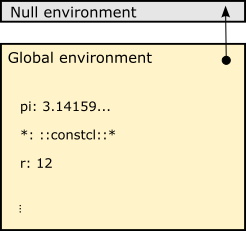
\includegraphics{images/env1.png}

During the call. Note how the global \texttt{r} is shadowed by the local one, and how the local environment links to the global one to find \texttt{*} and \texttt{pi}.

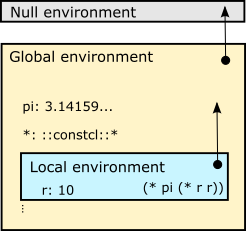
\includegraphics{images/env2.png}

After the call, we are back to the first state again.

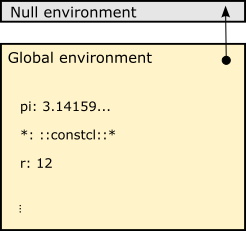
\includegraphics{images/env1.png}
\chapter{Initialization}
\label{initialization}


Initialize the memory space for vector contents.

\begin{lstlisting}
set ::constcl::vectorSpace [lrepeat 1024 #NIL]
 
set ::constcl::vectorAssign 0
 
proc ::constcl::vsAlloc {num} {
  # TODO calculate free space
  set va $::constcl::vectorAssign
  incr ::constcl::vectorAssign $num
  return $va
}
\end{lstlisting}
\begin{lstlisting}
set ::constcl::gensymnum 0
\end{lstlisting}


Pre-make a set of constants (e.g. \#NIL, \#t, and \#f) and give them aliases for use in source text.

\begin{lstlisting}
interp alias {} #NIL {} [::constcl::NIL new]
 
interp alias {} #t {} [::constcl::MkBoolean #t]
 
interp alias {} #f {} [::constcl::MkBoolean #f]
 
interp alias {} #-1 {} [N -1]
 
interp alias {} #0 {} [N 0]
 
interp alias {} #1 {} [N 1]
 
interp alias {} #+ {} [::constcl::MkSymbol +]
 
interp alias {} #- {} [::constcl::MkSymbol -]
 
interp alias {} #UNS {} [::constcl::Unspecified new]
 
interp alias {} #UND {} [::constcl::Undefined new]
 
interp alias {} #EOF {} [::constcl::EndOfFile new]
\end{lstlisting}


Initialize the definition register with the queen of numbers (or at least a double-precision floating point approximation).

\index{pi}
\begin{lstlisting}
dict set ::constcl::defreg pi [N 3.1415926535897931]
\end{lstlisting}


In this interpreter, \texttt{nil} does refer to the empty list.

\index{nil}
\begin{lstlisting}
reg nil #NIL
\end{lstlisting}
\section{Environment startup}
\label{environment-startup}
\index{environment startup}


On startup, two \texttt{Environment} objects called \texttt{null\_env} (the null environment, not the same as \texttt{null-environment} in Scheme) and \texttt{global\_env} (the global environment) are created.


Make \texttt{null\_env} empty and judgemental: this is where searches for unbound symbols end up.

\index{null\_env}
\begin{lstlisting}
::constcl::Environment create \
  ::constcl::null_env #NIL {}
 
oo::objdefine ::constcl::null_env {
  method find {sym} {
    self
  }
  method get {sym} {
    ::error "Unbound variable: [$sym name]"
  }
  method set {sym val} {
    ::error "Unbound variable: [$sym name]"
  }
}
\end{lstlisting}


Meanwhile, \texttt{global\_env} is populated with all the definitions from the definitions register, \texttt{defreg}. This is where top level evaluation happens.

\index{global\_env}
\begin{lstlisting}
namespace eval ::constcl {
  set keys [list {*}[lmap key [dict keys $defreg] {
    S $key
  }]]
  set vals [dict values $defreg]
  Environment create global_env $keys $vals \
    ::constcl::null_env
}
\end{lstlisting}


Load the Scheme base to add more definitions to the global environment.

\index{schemebase}
\begin{lstlisting}
pe {(load "schemebase.scm")}
\end{lstlisting}


Thereafter, each time a user-defined procedure is called, a new \texttt{Environment} object is created to hold the bindings introduced by the call, and also a link to the outer environment (the one closed over when the procedure was defined).

\chapter{The REPL}
\label{the-repl}


The REPL (read-eval-print loop) is a loop that repeatedly \emph{reads} a Scheme source string from the user through the command \texttt{::constcl::input} (breaking the loop if given an empty line) and \texttt{::constcl::parse}, \emph{evaluates} it using \texttt{::constcl::eval}, and \emph{prints} using \texttt{::constcl::write}.



\textbf{input}


\texttt{input} is modelled after the Python 3 function. It displays a prompt and reads a string.

\index{input}
\begin{lstlisting}
proc ::constcl::input {prompt} {
  puts -nonewline $prompt
  flush stdout
  set buf [gets stdin]
  set openpars [regexp -all -inline {\(} $buf]
  set clsepars [regexp -all -inline {\)} $buf]
  set openbrak [regexp -all -inline {\[} $buf]
  set clsebrak [regexp -all -inline {\]} $buf]
  while {[llength $openpars] > [llength $clsepars] ||
         [llength $openbrak] > [llength $clsebrak]} {
    ::append buf [gets stdin]
    set openpars [regexp -all -inline {\(} $buf]
    set clsepars [regexp -all -inline {\)} $buf]
    set openbrak [regexp -all -inline {\[} $buf]
    set clsebrak [regexp -all -inline {\]} $buf]
  }
  return $buf
}
\end{lstlisting}


\textbf{repl}


\texttt{repl} puts the 'loop' in the read-eval-print loop. It repeats prompting for a string until given a blank input. Given non-blank input, it parses and evaluates the string, printing the resulting value.

\index{repl}
\begin{lstlisting}
proc ::repl {{prompt "ConsTcl> "}} {
  set cur_env [Environment new #NIL {} ::global_env]
  set str [::constcl::input $prompt]
  while {$str ne ""} {
    set expr [::constcl::parse $str]
    set val [::constcl::eval $expr $cur_env]
    ::constcl::write $val
    set str [::constcl::input $prompt]
  }
  $cur_env destroy
}
\end{lstlisting}

\printindex
\end{document}

